%%%%%%%%%%%%%%%%%%%%%%%%%%%%%%%%%%%%%%%%%%%%%%%%%%
%\documentclass[a4paper,12pt]{jarticle}%
\documentclass[platex,a4paper,12pt]{jsarticle}%
%\documentstyle[pre,aps]{revtex}

\setlength{\textheight}{\paperheight}   % ひとまず紙面を本文領域に
\setlength{\topmargin}{-5.4truemm}      % 上の余白を20mm(=1inch-5.4mm)に
\addtolength{\topmargin}{-\headheight}  % 
\addtolength{\topmargin}{-\headsep}     % ヘッダの分だけ本文領域を移動させる
\addtolength{\textheight}{-40truemm}    % 下の余白も20mmに
%% 幅の設定
\setlength{\textwidth}{\paperwidth}     % ひとまず紙面を本文領域に
\setlength{\oddsidemargin}{-5.4truemm}  % 左の余白を20mm(=1inch-5.4mm)に
\setlength{\evensidemargin}{-5.4truemm} % 
\addtolength{\textwidth}{-40truemm}     % 右の余白も20mmに

\usepackage{wrapfig}
%\usepackage[dvips]{graphicx}
%\usepackage[dvipdfmx]{graphicx}
\usepackage{graphicx}

\usepackage{url}

\usepackage[usenames]{color}
%\usepackage{jumoline}
\usepackage{color}
\usepackage{ascmac}
\everymath{\displaystyle}

\usepackage{comment}

\usepackage{amssymb}

\usepackage{fancyhdr}
\pagestyle{fancy}
\lhead{}
\rhead{}
\rhead{\thepage{}}
\cfoot{}
\renewcommand{\headrulewidth}{0pt}

%
\baselineskip 9mm

%\pagestyle{empty}
\title{\vspace{10mm}\Huge{GLSC3D (Ver. 3.0.0) \\ Manual}}
\author{\Large{構想・制作・監督:秋山 正和}\\\vspace{5mm}
北海道大学 電子科学研究所 \vspace{1zw} \\
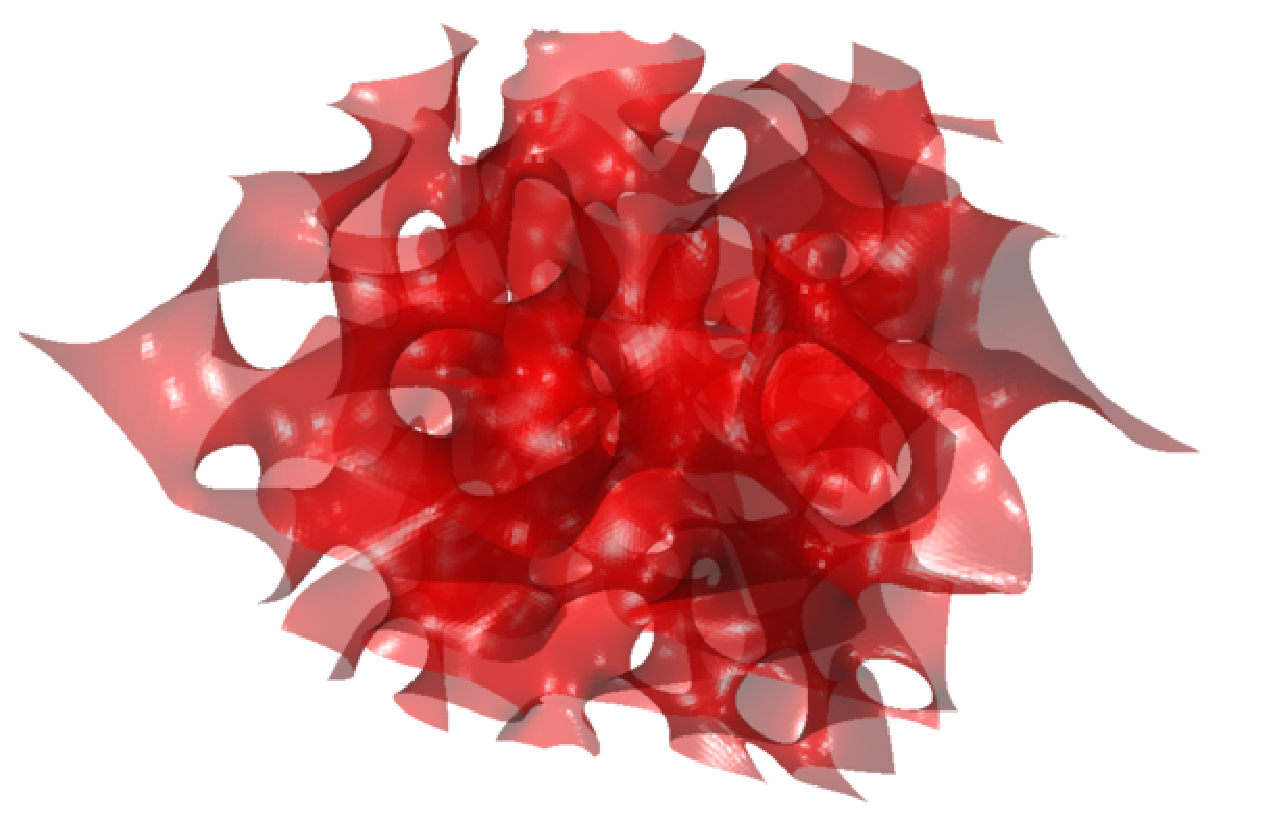
\includegraphics[width=100mm]{Figures/eps/CoverPage.eps} \vspace{1zw} \\
\Large{制作(Ver. 2.2.1以降):舘入 数磨$^*$,須志田 隆道$^\dagger$} \\
$^*$北海道大学大学院 理学研究院 数学専攻,  $^\dagger$北海道大学 電子科学研究所
\vspace{1zw}\\ 
\Large{制作(Ver. 2.2.1まで):平芳 悠人,岡本 守} \\
北海道大学 理学部 数学科\\
\\
\\
\date{\today}
}

\begin{document}

\maketitle
\thispagestyle{empty}

%%%%%%%%%%%%%%%%%%%%%%% 白紙ページ %%%%%%%%%%%%%%%%%%%%%%%%%%%

\newpage
\thispagestyle{empty}
 
\newpage

%%%%%%%%%%%%%%%%%%%%%%% 目次 %%%%%%%%%%%%%%%%%%%%%%%%%%%%%%%
\setcounter{tocdepth}{3}
\tableofcontents

%%%%%%%%%%%%%%%%%%%%%%% 白紙ページ %%%%%%%%%%%%%%%%%%%%%%%%%%%%%
\newpage
\thispagestyle{empty}
 
\newpage

%%%%%%%%%%%%%%%%%%%%%%% 本文 %%%%%%%%%%%%%%%%%%%%%%%%%%%%%
\section{はじめに}

本章ではGLSCの歴史やGLSC3Dの開発に至る経緯などを詳しく紹介します.手っ取り早く使いたい方は本章を読み飛ばしください.

\subsection{GLSCとその歴史}

GLSC とは,Graphics Library for Scientific Computing の略で,科学計算の結果をディスプレイ上に表示するための簡単なグラフィックライブラリです\footnote{``GLSC 小林 亮"とgoogle検索するか,
\url{http://www-mmc.es.hokudai.ac.jp/~masakazu/}を見てください}.GLSCは小林 亮氏,高橋 大輔氏,中野 浩氏,松木平 淳太氏によって開発されました.当時(1980年頃)はコンピュータ環境こそ整っていましたが,その計算結果を可視化する汎用のソフトウェアが殆どありませんでした.そのような時代に,「ユーザーに出来るだけ負担をかけずに簡単に数値計算結果を可視化したい」という目的でGLSCは開発されました.今日では,計算結果を可視化するソフトウェアはgnuplot \footnote{\url{http://www.gnuplot.info/}}を始め,Mathematica, MatLab\footnote{Mathematica, Matlabは数式処理や簡単な数値計算もできるので,可視化ソフトというよりは「可視化もできる」ソフトというべきですね.}など様々なものがあります.したがって「GLSCを使わなければ,可視化はできないか?」と問われれば答えはNoとなります.しかしながら,今でもGLSCにはコアなファン\footnote{もっとも授業などで最初に習った言語はその後を引きずるので,その影響で仕方なくという方もいるでしょうが...}が沢山います.では,どのような点がGLSCは優れているのでしょうか?

\subsection{GLSCの長所・短所}

我々,数理科学者は現象と向き合い,数理モデルを作成しながら現象を理解することを生業としています.そして構成された数理モデルは,解析的に解くことは困難です.したがって,解を表示したりするためには,数値計算を行いのその結果を可視化するしかありません.この時多くの場合,数値計算のコードが先に出来上がります.次にそれをグラフィカルに表示するためにグラフィック用のコードを作成します.

ランダムウォークを例に取りましょう.次のページにランダムウォークを計算するCコードを貼りつけてあります.\verb|r[i]|は\verb|i|番目の粒子の位置(整数値)を示します.19行目まで計算することによって,変数\verb|r[i]|の値が更新されます.計算の結果がうまく行われているかを確認するために,21行目以降ではそれらを端末に表示するコードが示されています.試しに計算をしてみましょう.結果がグラフィカルに表示されていないので,わかりにくいと感じるはずです.そこで多くの場合,この結果を何らかの可視化ソフトを用い可視化します.先にも示したように,Freeで手に入り,マニュアルも豊富に存在するということで,gnuplotは最近人気です.先の実行ファイルに対し,リダイレクション``$>$''を用いることで,計算結果を他のファイルに記録することができます.gnuplotにはこのデータを与えて可視化を行います.gnuplotは「与えられた座標に点を打つ」,「点どうしを先で結ぶ」,「鳥瞰図を作成する」など基本的な可視化を行うことができます.先の例では,端末での表示を見やすくするために計算結果に

\verb|---------------- Step = 0 ----------------|

\newpage

\begin{verbatim}
  1 #include <stdio.h>
  2 #include <stdlib.h>
  3 #define     N       (10)
  4 #define     STEP    (100)
  5 int PlusMinus(void)
  6 {
  7     if(rand() < RAND_MAX / 2) return  1;
  8     else                      return -1;
  9 }
 10 int main(void)
 11 {
 12     int         i, r[N],i_time;
 13     //Initialize
 14     for(i = 0;i < N;i ++) r[i] = 0;
 15     //Time Loop
 16     for(i_time = 0;i_time < STEP;i_time ++)
 17     {
 18         //Calc
 19         for(i = 0;i < N;i ++) r[i] += PlusMinus();
 20         //Print
 21         printf("---------------- Step = %d ----------------\n",i_time);
 22         for(i = 0;i < N;i ++) printf("%3d ",r[i]);
 23         printf("\n");
 24     }
 25     return 0;
 26 }
計算結果
---------------- Step = 0 ----------------
  1   1  -1   1  -1   1   1  -1  -1  -1 
---------------- Step = 1 ----------------
  2   0  -2   2   0   0   0   0   0   0 
---------------- Step = 2 ----------------
            :
            :
---------------- Step = 98 ----------------
 -5 -15  13   1  -7  15  -3   1   7  -3 
---------------- Step = 99 ----------------
 -4 -16  12   2  -8  14  -4   0   6  -2 
\end{verbatim}

\noindent
などと表示をしていましたが,gnuplotではこのような文字列は受け付けません.よって,多くの場合,gnuplotに適するように計算結果をフォーマットし直す必要があります.この例でもわかるように,数値計算のコードを書いた後に可視化のコードを書くということが,多くの現場で行われていることでしょう.

この方法には大きな欠点があります.それは「リアルタイムに可視化できていない」という問題です.先の例では,数値計算はほんの一瞬で終わりますが,中には長時間の計算を必要とする場合もあります.そのような場合,「計算と同時に可視化もできたらいいのに」と多くの人は思うことでしょう.もちろん,gnuplotではpopen関数を用いて,C言語から直接gnuplotを呼ぶこともでき,この目的を達成出来ます.しかしながら,数値計算のコードよりも可視化のコードの部分が肥大化するという問題がよく起こります.この問題も,できるだけコードが肥大化しないように,プログラマが適切に関数を作ればよいのですが,C言語からgnuplotを簡単かつスマート呼べるようなツールはないようです\footnote{2014.6.4原稿作成時時点}.GLSCはC言語から非常に簡単に呼ぶことができるように設計されており,数値計算をしながらリアルタイムに可視化を行うことが可能です.また,GLSCは内部でX Windowsy System\footnote{http://www.x.org/}を使用しており,描画も非常に高速である長所があります.

\begin{wrapfigure}[10]{r}{70mm}
\vspace{-1\baselineskip}
	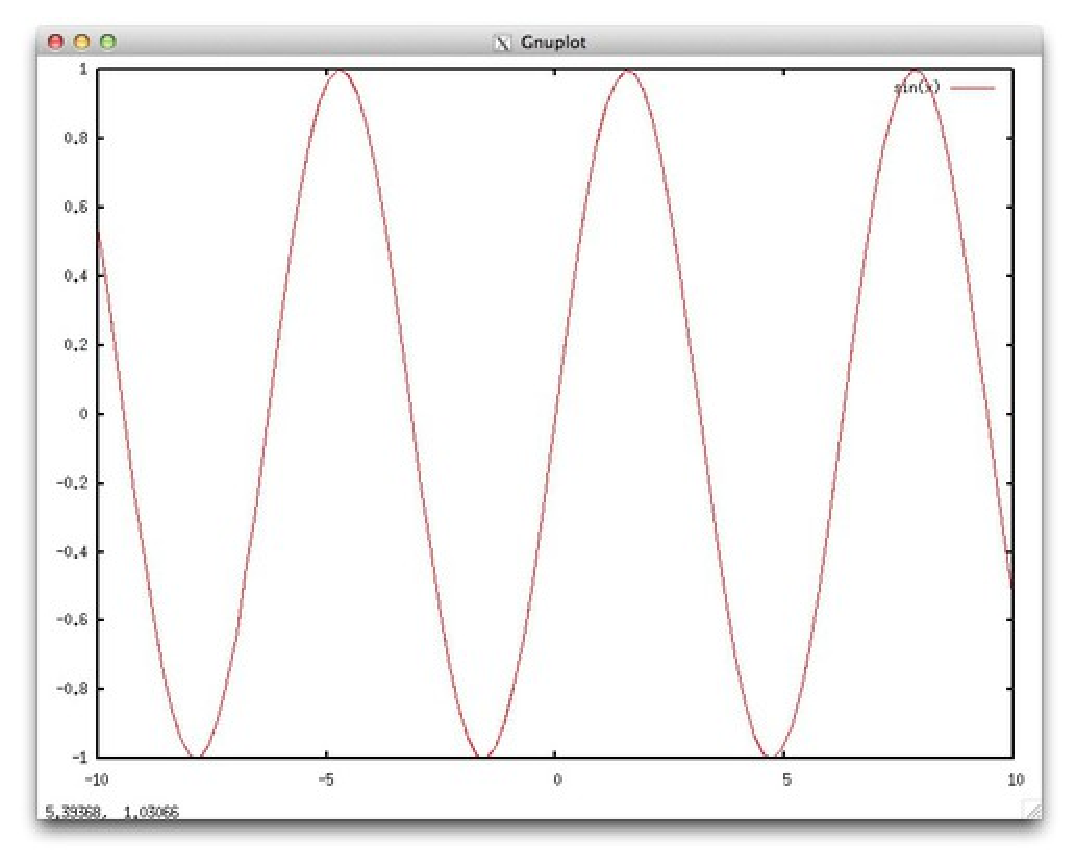
\includegraphics[width=70mm]{./Figures/eps/001.eps}
\end{wrapfigure}

その一方で,GLSCには短所もあります.例えば,gnuplotなどの汎用ツールは次のように端末に打つとグラフを出します.

\noindent
\verb|gnuplot> plot sin(x)|

\noindent
グラフが出るだけでなく,軸,目盛り,関数の名前など様々な情報を付加してくれます.これはgnuplotが内部的に適切に処理をしてくれているお陰です.しかしながら,GLSCにはそのようなものはありません.そのような付加情報を出したければユーザー自身が直接コードを書かねばなりません.多くの方はこのような点を挙げ「GLSCはそのような機能がついていないのがやだ」,「自分で書くのが面倒だ」と批判的になります.確かにそのような側面はありますが,逆に言えば「なんでもできる」ということになります.やや脱線しますが,開発者の小林亮氏から次のような話を聞いたことがあります.

\noindent
「GLSCは確かになんでもはやってくれない,でも自由度が高い分,「ああしたい」,「こうしたい」という痒い所に手が届くんだ」

\noindent
なるほど,含蓄のあるお言葉です.

どんなツールにも短所と長所があります.ですから``GLSCでないとできない事''というのは,今日ないでしょう.しかしながら,GLSCは``数値計算のプロ''たちが,自身の経験から使いやすい形にまとめた関数の集大成となっています.つまりメインの数値計算のコードに``程よい程度の困難さで,ユーザーの思い描く自由なグラフィック発想を追加できる''という点がGLSCの長所なのです.
\subsection{GLSC3Dの開発まで}

長所と短所の話をした後ですが,GLSCには致命的な問題がありました.それは3次元空間の描画を扱えない\footnote{もちろん鳥瞰図や,等値面を描く関数はありますが...}ということです.GLSC開発当時,3次元計算を行うことは当時のスパコンでも大変でしたし,ましてや数値計算と同時に3次元の可視化をする必要もありませんでした.しかしながら,今日ではそのような話は普通に聞きます.作者は博士論文作成時\footnote{2010年の冬頃},非常に多くの3次元の数値計算を行っていましたが,GLSCでは可視化ができず\footnote{もちろん,3次元データから2次元の断片データをいくつか作り,可視化をすることは出来ましたが...},泣く泣く他の描画ツールを使った覚えがあります.その描画ツールはまったく痒い所に手が届かず,苦い経験をしたものです.その後も様々な文献を読み漁ったり,人に聞いたりして,使いやすそうな3次元可視化ツールを模索しました.数年模索をしましたが,結論から言えばそのようなツールはない,もしくはあっても非常に高い\footnote{AVSという有名な可視化ソフトがあります.教育向けの一番安いのでも15万円以上はします.Mathematicaも20万円はします...}ということでした.しかもそのようなソフトは,予想されたように,痒いところに手が届かなかったり,描画が非常に遅いという欠点もありました.``3次元の良い描画ツールがないために,研究が滞る''ということを避けるためにも,何らかの手を打たなければならない.そこで,筆者はGLSC3Dの開発に着手しました.

\subsubsection{X Window Systemの限界}
GLSC3Dとはその名の通り,GLSCの3次元への拡張バージョンのことです.GLSC3Dの基本的な思想や設計方針はGLSCと同じになるように設計されるべきです.このため,開発当初は新たな3Dの新関数をGLSCに追加する形で進められました\footnote{その名残がGLSC3.8世代にて追加された\verb|g_contln_3d|などです}.しかしながら,GLSCは内部的にX Window SystemをCallするため,新たに追加できる3D機能はX Window Systemの許す制限までということになります.X Window Systemは優れたライブラリですが,3次元の描画関数が乏しく,この路線での拡張は原理的に不可能と判断しました.そこで,他の描画ライブラリの使用を検討しました.

\subsubsection{OpenGLとGLUTの使用}
3次元の描画ライブラリとして有名なのは,やはりOpenGL(Open Graphics Library)\footnote{\verb|http://www.opengl.org/|}でしょう.DirectX\footnote{\verb|http://ja.wikipedia.org/wiki/Microsoft_DirectX|}というライブラリも有名ですが,Windows上でしか動かないので問題です.OpenGLは様々な環境で動作すること,描画が高速であること,そしてその名の通りオープンなAPI(Application Program Interface)であることから,GLSC3Dの構築には最適です.

OpenGLはグラフィック専門のAPIなので,ウインドウを画面に出したり,マウスやキーボードのようなデバイスから操作を受け付けるためには他のライブラリを使用する\footnote{このように書くとGLSC3Dではマウスやキーボードを使ってインタラクティブにグラフィックを行うことができそうですが,現時点(2014.6.5)ではそのような関数は未実装です.その後Ver2.2.1で実装されました.}必要があります.それがGLUT(OpenGL Utility Toolkit)\footnote{\verb|http://www.opengl.org/resources/libraries/glut/|}です.GLUTはこのようなOS間でのデバイスの違いの差も吸収してくれます.そこでOpengGLでインタラクティブなグラフィックプログラムを制作するといえば,大抵はGLUTも使用することになります.

実はGLUTは1998 年に発表された Version 3.7以降整備が行われなくなってしまいました.それでは困るということで,いくつかの団体(OpenGLUT\footnote{\verb|http://openglut.sourceforge.net/|},FreeGLUT\footnote{\verb|http://freeglut.sourceforge.net/|})がGLUTと互換性のある新たなライブラリを開発してきました.どちらの団体でも良かったのですが,freeGLUTのほうが作者の開発環境であるMacOSと相性がよいので,GLSC3Dの開発ではfreeGLUTを採用しました\footnote{何年か後にOpenGLUT陣営が勝っていれば,それに合わせてプログラムを更新します...}\footnote{FreeGLUTはいくつかの問題があることがわかり,Ver3.00からはSDLに移行されました.}.これにて,GLSC3Dの開発に必要な土台は準備出来ました.あとは,どのように実装するかという問題が残されました.

\subsubsection{GLSCらしさとOpenGLらしさ}

\begin{wrapfigure}[11]{r}{70mm}
\vspace{-1\baselineskip}
	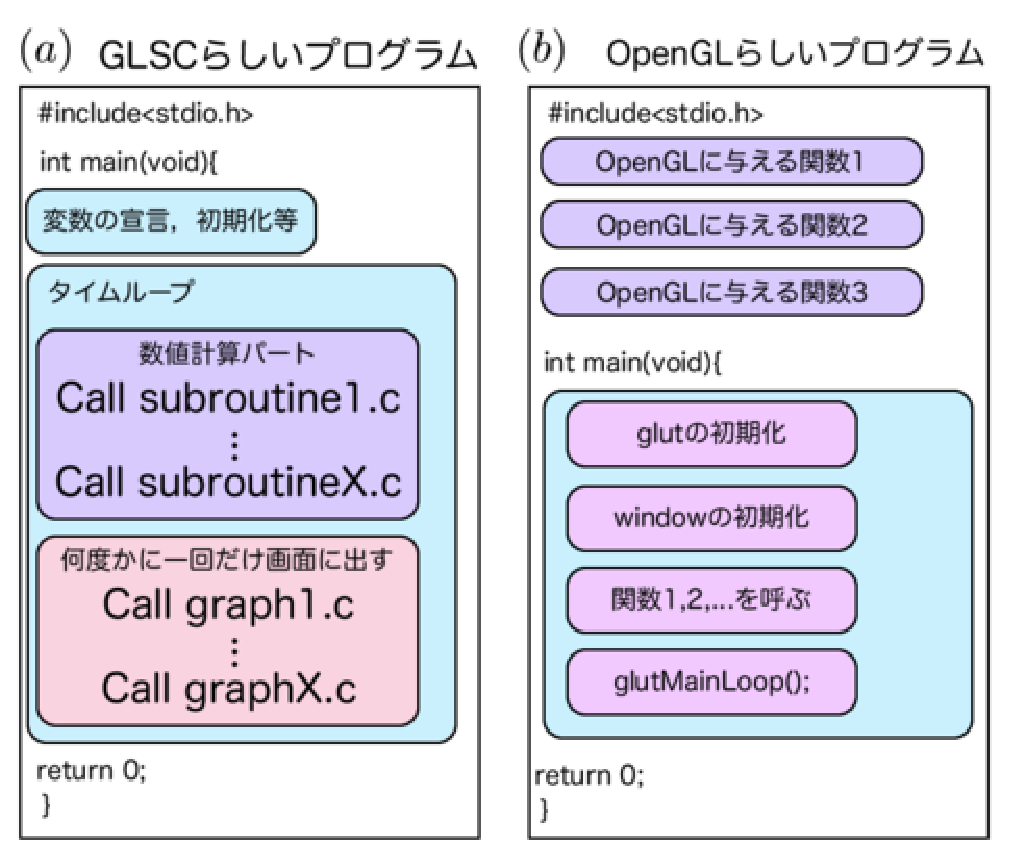
\includegraphics[width=70mm]{./Figures/eps/002.eps}
\end{wrapfigure}

先にも説明したように,GLSCは数値計算屋さんの作った描画ライブラリです.筆者は何かプロジェクトをスタートさせる時,数値計算のプログラムパートに精力を注ぎ,次にグラフィックパートを作成します\footnote{こう言うとグラフィックを疎かにしているようですが,グラフィックも綺麗にしないとインパクトのある講演はできませんからね...どっちも大事です.}.この時,数値計算を行いながら,可視化を行うわけですから,必然的にプログラムは$(a)$の様な構成になります.ここではこのようなプログラミング構成をGLSCらしいプログラミング構成と定義します\footnote{「らしさ」を強要しているわけではありません.自由な発想に基づきプログラムをしてください.}.

さて,OpenGLのサンプルプログラムが載っている教科書等を一度読んでみてください.きっとプログラム構成は$(b)$のようになっていると思います.すなわちOpenGLやGLUTの関数の準備を行い,それらをmain関数内で呼ぶような構成です.そして一番のポイントは\verb|glutMainLoop|関数が呼ばれているということです.\verb|glutMainLoop|はコールバック関数と呼ばれる特殊な関数です.この関数は「プログラムの実行中,何かが起こった時に」登録された関数を呼び出す(呼び戻す)ことができるような関数です.具体的にいえば,マウスなどで3Dグラフィックを回転させたい時がありますが,そのようなイベントが発生した時に(つまりマウスの動きを察した時),OpenGL関数に対して「再描画せよ」と命令するのです.OpenGLはグラフィックをプログラミングするために適したAPIですので,このようなプログラミング構成になるのは至極当然のことです.私は今まで仕事柄,多くの人のプログラムを読んできましたが,OpenGLらしいプログラミング構成の中に,何とか数値計算のコードを潜り込ませ,実行させているのをよく見かけます.しかしながら,上記のように整理すればわかるように,このようなOpenGLらしいプログラミング構成とGLSCらしいプログラミング構成とは相容れない関係なのは明白です.OpenGLの参考文献に載ってるいるような「サンプルを数カ所変更すればGLSC3Dが完成!」というわけにはいかなかったからです.GLSC3Dの開発は困難を極めました.

\subsubsection{GLSC3Dの赤ちゃんの誕生}

GLSCらしいプログラミング構成となるように,どのようにOpenGLの関数を呼び,GLSC3Dの設計をすればよいのかは長らく未解決でした.ある時,研究室の樋口亮君ととある研究を行う中で,彼のOpenGLのプログラムをぼーっと見ていました.その時,このコードの一部に,これを解決するような構成方法を発見しました\footnote{樋口君,会社員になっても元気か?ついに開発したぞ!}.筆者はこのコードと発見こそがGLSC3D開発に大きく貢献したと思います.この場を借りて,樋口君には感謝の意を捧げます.

\subsection{GLSC3Dの開発}

\begin{wrapfigure}[6]{r}{30mm}
\vspace{-1\baselineskip}
	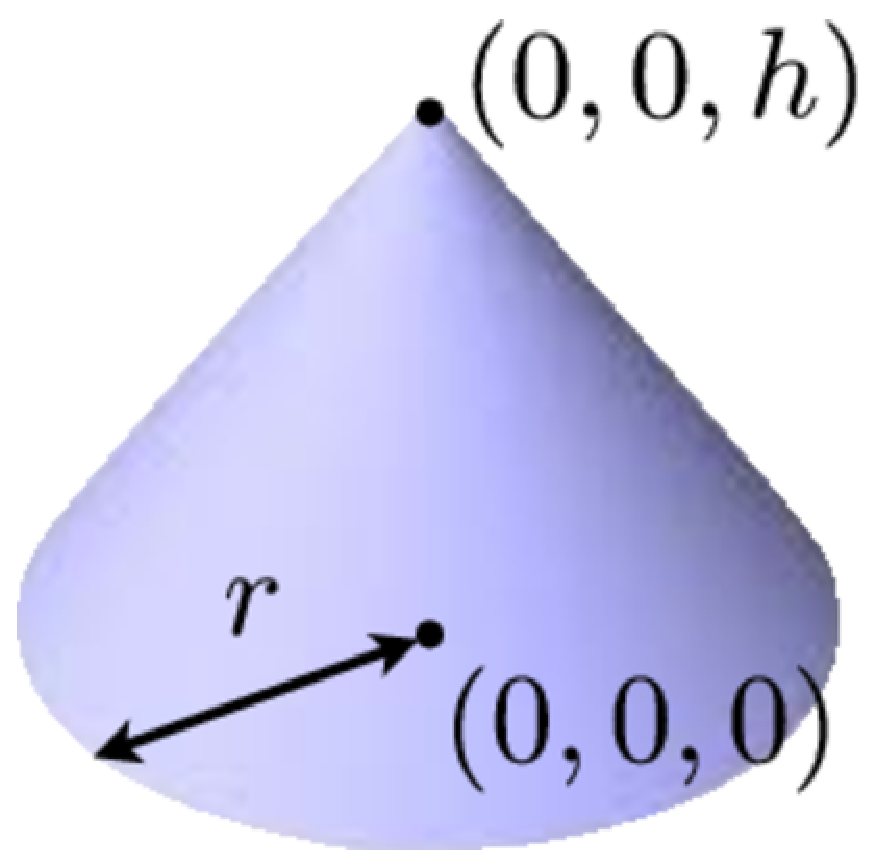
\includegraphics[width=30mm]{./Figures/eps/003.eps}
\end{wrapfigure}

GLSC3Dの根幹部分は先が見えたので,あとは実際の描画関数の設計を行うことを考えます.例えば,円錐を描画する関数\verb|DrawCone|を考えます.円錐の底の中心が原点$(0,0,0)$,尖った先端を$(0,0,h)$,円錐の半径を$r$として円錐の描画関数を設計することを考えます.\verb|DrawCone|の引数\footnote{引数(ひきすう)と読みます.例えば関数$f(x,y)$なら$x,y$が引数です.とある学生がこの漢字を読めなかったもので...}は$h,r$ということになります.当たり前ですが,この状態で描画される円錐はいつも底の中心が原点となっていますし,傾いた円錐というのも描画できません.このような時,3Dオブジェクトに対して平行移動や回転などを施してやれば目的を達成できます.しかしながら\verb|DrawCone|は呼ばれた時点で,底の中心が原点となるようなものしか描画できません.どうすればよいでしょうか.一つの戦略は\verb|DrawCone|関数の引数を増やし,円錐の底の座標や傾きなどを追加し,\verb|DrawCone|の内部設計を変える方法です.でも,これは開発者側はちょっと面倒なプログラミングをせねばなりません.

二つ目の戦略はOpenGLに用意されている

\noindent
\verb|glPushMatrix, glPopMatrix, glTranslatef, glRotatef|

\noindent
などの関数を使うことです.詳細は他書\footnote{OpenGLプログラミングガイド 原著第5版など}に委ねますが,簡単にいえば標準的な位置・方向の3Dオブジェクトに対して平行移動や回転などを施して,{\bf 描画時}に傾かせたり,移動させて見せたりする方法です.この方法はグラフィックスをメインとするようなプログラミング作成の際にはよく使われる手法です.しかしながら,GLSC3Dはあくまでも数値計算をメインとするような人向けのツールです.したがって,この手のやり方をユーザに強制するのはいかがなものか?ということになりました.そこで,GLSC3Dでは戦略1をとりました.戦略1は関数の引数が多くなり,開発に手間がかかるという欠点はありますが,3Dオブジェクトの描画を任意の位置や方向に制御可能です.引数が多いなと感じる方もいるとは思いますが,試行錯誤の末,削りに削ったものです.もし,気に入らなければ,引数の少ない描画関数を自身で設計することも可能です.

このような経緯がありましたが,当面の問題は解決されGLSC3Dの開発はスタートしました.

\subsection{GLSC3Dの設計哲学}

GLSC3DはGLSCと同じ設計哲学を有します.それはおよそ以下の様な設計哲学です.

\noindent {\bf 数値計算のコードを邪魔しない}

先の述べたように,多くの場合数値シミュレーションのプログラムは,根幹をなす数値計算コードの部分が先に完成され,その後描画のパートが作成されます.したがってGLSC3Dはもとの数値計算コードの部分に大きな変更を求めたり,後からの追加が困難であるように設計されてはなりません.したがって簡単な手続きで,GLSC3Dのコードをもとのコードに埋め込めることができるように設計されるべきです.

\noindent {\bf 関数の引数は必要最低限にせよ}

関数の引数は多ければ多いほど豊かな動作が可能です.しかしながら,関数の引数が多いと「この関数の引数はなんだっけ?順番はどうだったっけ?」という問題が発生し,マニュアルとにらめっこしなければなりません.したがって関数の引数は,「その関数の動作に支障きたさない範囲内で最低限のレベルまで減らす」ことが求められます.例えば球を描画する場合はどのように工夫をしても,中心座標と半径は引数として必要でしょう.したがって\verb|g_sphere_3D|関数はこのような引数を必須としています.一方で\verb|g_sphere|で球を描画していると,「ゴツゴツしているのでもう少しなめらかな球を描きたい,ワイヤーフレームで描きたい,etc...」といった欲望が出てくる場合もあります.そのような場合に備えてGLSC3Dでは,ほとんどすべての関数に添字``\verb|_core|''のついた上位版の関数を用意しています.例えば\verb|g_sphere_3D_core|は球面の分割レベル,面の三角形分割のレベル,ワイヤフレームにするかどうかなどを指定することができます(詳細は関数の説明を御覧ください).GLSC3Dでは一般に関数\verb|g_A|, \verb|g_A_core|が存在する場合\verb|g_A|は内部的に\verb|g_A_core|をCallしています.

\noindent {\bf だからと言って構造体などで包まない}

構造体を使えば,一つの構造体を関数に渡せばあたかも多数の引数を渡したことと同等のことが実現できます.しかしながら,この方法も結局「この関数の構造体のメンバーはなんだっけ?型の名前はなんだっけ?」という問題が発生し,マニュアルとにらめっこしなければなりません.そのようなことからGLSC3Dでは構造体を通して引数を渡すことをしません.もし「引数が多くて嫌だな...」と思われる場合は,ユーザー自身で構造体を作成しGLSC3Dの関数をラッピングしてご使用ください.\footnote{とは言っても3次元の計算ツールなので,座標ぐらいは構造体にしたい気分です.そのうちリリースするかもしれません}

\noindent {\bf ユーザーが自由に関数を設計できる}

先に\verb|g_sphere_3D|を例にしましたが,例えば「球面の北極部分を赤く,南極部分を青く,さらに赤道部分は緑にしたい」という欲望が出た場合,\verb|g_sphere_3D_core|ではもはや手におえません.GLSC3Dは「ユーザーが自由に関数を設計できるよう」に設計されるべきです.したがって一番細かいレベルの目的を達成できるようなプリミティブな関数を提供すべきです.GLSC3Dでは点を打つ,線を描く,面を描く,文字を書くといったような基本的な関数群を揃えてありますので,それを組み合わせて使用することで,どんな関数でも設計することが可能です.これらの使用方法を熟読し自由な発想で描画を楽しんでください.

%%%%%%%%%%%%%%%%%%%%%%%%%%%%%%%%%%%%%%%%%%%%%%%%%%%%%%%%%%%%%%%%%%%%%%%%%%%
\newpage
\section{GLSCおよびGLSC3D Ver2.xからの変更点及び注意点}

GLSC3DはGLSCの設計哲学を引き継ぎ構築されています.理想的には,関数の命名規則,引数などがシームレスに繋がり,ユーザには「どこが変わったかわからない」と思わせるように設計すべきです.しかしながら,それぞれの基盤ライブラリであるOpenGLとX Window Systemは全く異なるものです.したがって,GLSC3Dの開発は0から作り上げていく方式を取らざるを得ませんでした.そして開発中,どうしても変更せざるを得ないくつかの点が生じました.また,3次元化されたこと及び新関数の導入によって,GLSCとは別の新たな注意点が発生しました.マニュアルの順番としてはGLSC3Dの関数を紹介した後に本章を置くべきですが,非常に重要な変更のため本章にてお知らせします.

\subsection{GLSCからの変更点}

\subsubsection{Fortran言語をサポートしていない}

GLSCではFortranをサポートしていましたが,GLSC3Dではサポートしていません.未来永劫に渡り,Fortranをサポートしないわけではありません.GLSC同様に内部的にはすべてをポインタ渡しにWrapするとで,FortranからCをCallできますので,Fortranに強い方でWrapperプログラムを書いてもいいよという方は筆者までお知らせください.

\subsubsection{最終の描画スタイルの変更}

3次元オブジェクトを描画する際,OpenGLでは描画命令をいくつかのまとまった単位になるまで保持し,一気に描画するというスタイルが取られます.また描画の最初と最後を明示的に指定しなければなりません(下記参照).\footnote{この方法はOpenGL 3.1 以降では廃止されておりVertex BufferとVertex Arrayを使用する必要があります.}

\begin{itembox}[l]{OpenGLの描画スタイル(3次元空間内で線分を描画する場合)}
	
	\verb|glBegin(GL_LINES);|	\hspace{20mm}/*線を描き始めることを指定*/
	
	\verb|glVertex3f(0,0,0);|		\hspace{20mm}/*線分の端点を指定*/
	
	\verb|glVertex3f(0,1,0);|		\hspace{20mm}/*線分の端点を指定*/
	
	\verb|glEnd();|				\hspace{38mm}/*線を描き終えたことを指定*/

	\verb|glFlush();|				\hspace{34mm}/*線を描く命令を実行*/
\end{itembox}

一方,GLSCで描画命令はその都度実行されます.したがって,描画の最初と最後を明示的に指
定する必要はありません(下記参照).

\begin{itembox}[l]{GLSCの描画スタイル(2次元空間内で線分を描画する場合)}
	
	\verb|g_move(0,0);|\hspace{30mm}/*線分の端点を指定*/
	
	\verb|g_plot(0,1);|\hspace{30mm}/*線分の端点を指定*/

\end{itembox}

GLSCのほうが記述が楽で良さそうに思えますが,描画命令がその都度実行されるので,OpenGLに比べ(若干ですが)描画が遅くなったり,画面がちらついたりする可能性があります.\footnote{OpenGLではちらつきを抑えるためにダブルバッファリングという手法を用いることができます.GLSC3Dはこの手法を用いています.}.

GLSC3DではGLSCの哲学とOpenGLの良さを引き継いでいますので,次のように書くことができます.

\begin{itembox}[l]{GLSC3Dの描画スタイル(3次元空間内で線分を描画する)}
	
	\verb|g_move_3D(0,0,0);|\hspace{30mm}/*線分の端点を指定*/
	
	\verb|g_plot_3D(0,1,0);|\hspace{30mm}/*線分の端点を指定*/
	
	\verb|g_finish();|\hspace{35mm}/*バッファの描画命令を実行*/

\end{itembox}
  
最後の\verb|g_finish|ですが,GLSCではなかった記述です.\verb|g_finish|はタイムループ内で描画関数が終わった時{\bf 最後に一度だけ}呼ぶ必要があります.この関数を呼ぶことで,今までバッファに溜まっていた描画命令が一気に実行されます.多くの場合,最終的な描画の後で画面を短い時間停止させます.GLSCではそのような場合,\verb|g_sleep|関数を用いていました.GLSC3Dでは最終的な描画の後で\verb|g_finish|を用いる必要がありますので,次のようにプログラミングすることが多くなるでしょう.これが大きな変更点です.

\begin{itembox}[l]{GLSC3Dの描画スタイル}
	
	\verb|g_xxxx;|\hspace{60mm}/*描画1*/
	
	\verb|g_xxxx;|\hspace{60mm}/*描画2*/
	
	\verb|g_xxxx;|\hspace{60mm}/*描画3*/
	
	\verb|.|
	
	\verb|.|
	
	\verb|.|
	
	\verb|g_finish();|\hspace{45mm}/*バッファの描画命令を実行*/

	\verb|g_sleep(0.05);|\hspace{40mm}/*0.05秒間停止する*/
\end{itembox}

\newpage
\subsection{GLSC3D Ver2.x からの変更点}

\subsubsection{OpenGL の最新規格への追随}
OpenGLは1992年に誕生しました.1990年代,GPUは決められた描画アルゴリズムしか実行できませんでした.
その後GPUは劇的に進化し,現在はシェーダーと呼ばれるGPU上で実行されるプログラムを用いてグラフィックスの表示を行うことが一般的となっております.

2008年にOpenGL 3.0が発表され,従来の固定機能に由来する大量のAPIが非推奨と宣言され,翌年のOpenGL 3.1で削除されました.
現在も古いバージョンのOpenGLは残されているため固定機能を使い続けることはできますが,将来にわたって存在が保証されているわけではありません.
GLSCはVer 3.0でOpenGLの最新バージョンと互換性を保つこととしました.

\subsubsection{ウインドウライブラリをFreeGLUTからSDLへの変更}
以前のGLSC3DではFreeGLUTを用いてウインドウを表示していました.

Mac OS X上ではFreeGLUTはネイティブに動作せず,代わりにXQuartzを用いてX Window System上で動作させる必要がありました.しかしXQuartzは
\begin{itemize}
	\item XQuartz上で利用できるOpenGLがバージョン2.1に限定されるため,\\非推奨な(OpenGL 3.1 以降廃止された)描画方法しかできない
	\item ウインドウのサイズ変更・最大化ができない
	\item Retina Display に対応していないため,MacBook Proなどでの表示が美しくない
	\item 起動が遅い
	\item XQuartz自体が将来にわたって存在するのかどうか怪しい
\end{itemize}
といった問題点があったため,使用するライブラリをFreeGLUTからSDLに変更しました.

\subsubsection{2Dの描画順の変更}
以前のGLSC3Dでは2Dで先に描画したものが後に描画したものより優先して表示されていました.
Ver 3.0以降では後に描画したものが優先して表示されるように変更しました.

なお,3Dモードの場合も奥行きが完全に一致したときには,同様の挙動になるように変更されています.

\subsubsection{フォント埋め込みの廃止,フォント指定関数の変更,日本語などのUnicode文字への対応}
以前のGLSC3Dでは4種類の日本語フォントをライブラリに埋め込んでいましたが,ファイルサイズが肥大化するためこれを廃止しました.
GLSC3D 3.0ではデフォルトのフォントを
\begin{table}[h]
	\centering
	\begin{tabular}{ll}
		Mac OS X & /System/Library/Fonts/ヒラギノ角ゴシック W4.ttc\\
		Linux & /usr/share/fonts/opentype/noto/NotoSansCJK-Regular.ttc\\
		Windows & C:/Windows/Fonts/Meiryo.ttc\\
	\end{tabular}
\end{table}

から読み込みます.もしこの場所にフォントが存在しない場合,または違うフォントを使いたい場合,\verb|g_text_font_core|にフォントファイル名を指定してください.
また,\verb|Source/g_text.cpp|内の\verb|DEFAULT_FONT_FILE|を書き換えてコンパイルし直せばデフォルトのフォントを変更することもできます.

埋め込みフォントを指定する関数\verb|g_text_font|を廃止しました.また,テキストのフォント指定\verb|g_text_font_core|とサイズ指定\verb|g_text_size|を分離しました.
また,\verb|g_def_text|関数の\verb|font|引数は無視されます.

日本語や数学記号などのUnicode文字に対応しました.これを用いる場合文字列のエンコードは必ずUTF-8にしてください.
gccでは文字列リテラルのエンコードはデフォルトでUTF-8になります.お使いのコンパイラーのデフォルトがUTF-8でない場合,
C++11の\verb|u8|プレフィックスを使用してみてください.(C++11としてコンパイルする必要があります)
\begin{center}
\verb|g_text_virtual_3D(0, 0, 0, u8"あいうえお");|
\end{center}

\subsubsection{ウィンドウのサイズ変更・最大化と Apple Retina Display の対応}
Ver 3.0以降ではウィンドウのサイズ変更・最大化と Apple Retina Display に対応しています.
このため,GLSC3Dは内部的にスケールファクターを保持しており,\verb|g_init, g_init_core|に渡されたウインドウサイズに対する現在のサイズの比率(の水平方向と垂直方向の値の小さいほう)を使用します.
スケールの対象になるのは次の関数です.
\begin{itemize}
	\item \verb|g_sel_scale_2D, g_sel_scale_3D|
	\item \verb|g_marker_size, g_line_width, g_text_size|
	\item \verb|g_text_standard|
	\item \verb|g_input_state| (マウス座標の逆変換)
\end{itemize}
Ver 3.0以降では\verb|g_sel_scale_2D, g_sel_scale_3D|を(最初に1回だけ呼ぶのではなく)ループ内で使用することをお勧めします.
これによりウインドウサイズの変更に適切に対応できるようになります.

\verb|g_capture|を用いる場合,ウインドウサイズの変更は行わないでください.

Apple Retina Display の対応はデフォルトでは無効になっています.
有効化する場合,\verb|g_enable_highdpi|を\verb|g_init(_core)|の前に呼び出してください.
この場合,スケールファクターの初期値は2になります.それ以外の場合,スケールファクターの初期値は1です.

\subsubsection{マーカーの種類の追加}
\verb|g_marker_type|として正方形,円のほかに球を指定できるようにしました.
引数には定数\verb|G_MARKER_SQUARE=0, G_MARKER_CIRCLE=1, G_MARKER_SPHERE=2|を指定できます.

球マーカーは3次元で小さな球を大量に描画する目的に最適化されており高速に動作します.
そのような目的では\verb|g_sphere_3D(_core)|を使用しないでください.

どの種類のマーカーでも,サイズは\verb|g_marker_size|によりピクセル単位の直径を指定できるほか,\verb|g_marker_radius|により仮想座標系での半径を指定することができます.

\subsubsection{その他}
Ver 3.0以降ではライトの最大数を3つに変更しました.
これは4つ以上のライトは不要と判断してのことですが,要望がある方は本マニュアルの ``おわりに'' をご覧ください.\\

\verb|g_init_core|に指定するウインドウの位置として,画面の中央に表示することを意味する\verb|G_WINDOW_CENTERED|を指定できるようにしました.
\verb|g_init|を使用した場合のウインドウの位置は常に\verb|G_WINDOW_CENTERED|となります.\\

多次元配列を受け取る関数
\begin{center}
	\verb|g_bird_view_3D, g_contln_2D, g_data_plot_3D, g_isosurface_3D|
\end{center}
はプリプロセッサマクロにより対応する1次元配列版
\begin{center}
	\verb|g_bird_view_f_3D, g_contln_f_2D, g_data_plot_f_3D, g_isosurface_f_3D|
\end{center}
に変換されるようにしました.今後はC++でも多次元配列版を使うことができます.

\newpage
\subsection{GLSC3Dの注意点}

\subsubsection{物体の透明化における注意点(Ver1.x をお使いの方へ)}

\begin{wrapfigure}[4]{r}{50mm}
\vspace{-1\baselineskip}
	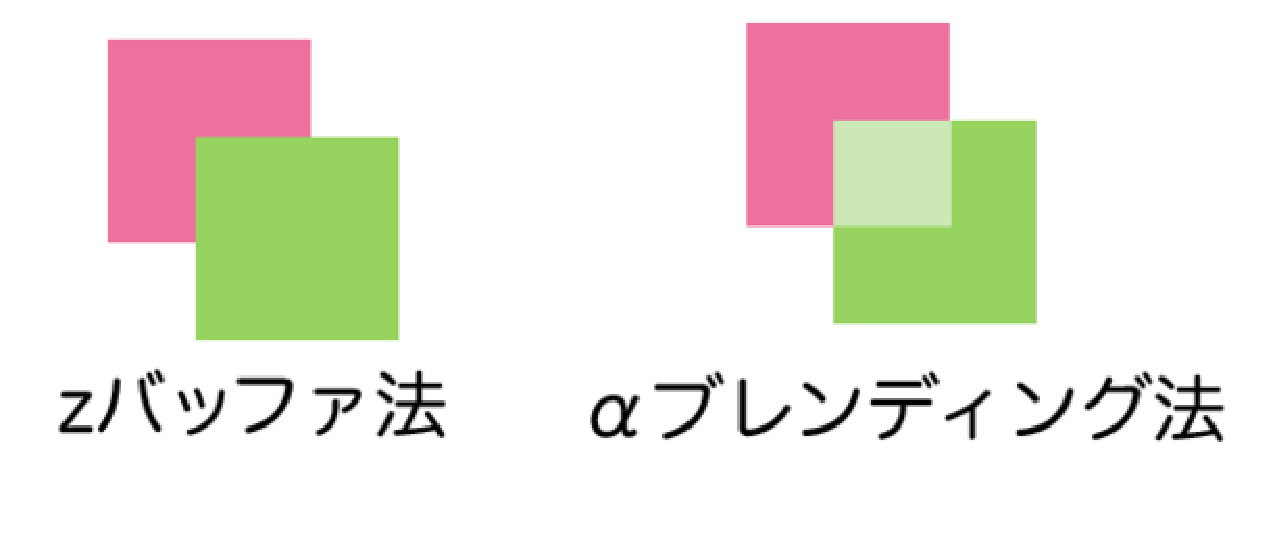
\includegraphics[width=50mm]{./Figures/eps/004.eps}
\end{wrapfigure}

2枚の板が重なっている状況を考えます.3次元では奥行き情報があるので,それを元にどちらが手前にあるかを判定し($z$バッファ法と呼ばれます)描画を行います.
GLSCでは物体の透明化処理はできませんでしたが,GLSC3Dでは$\alpha$ブレンディング法を用いて透明化処理を行うことができます.$\alpha$ブレンディング法はオブジェクトとオブジェクトが重なるとき,視点に対して手前にあるオブジェクトの色を,奥にあるオブジェクトの色と混ぜ合わせ描画することによって,透明化処理を行います.この事からわかるように,$\alpha$ブレンディング法は$z$バッファ法と同時に使うことは原理的に不可能です.そこで,$\alpha$ブレンディング法を使用する際は,$z$バッファ法はOFFにし,視点に対して奥の方から先に3Dオブジェクトの描画を行う必要があります.GLSC3Dでは$\alpha$ブレンディング法を使用する際に自動的に$z$バッファ法はOFFになり\footnote{GLSC3Dでは$\alpha$ブレンディング法の使用が終わると$z$バッファ法は自動的にONになります.つまり$\alpha$ブレンディング法が特別扱いにされています.}ますが,{\bf 視点に対して奥の方から先に3Dオブジェクトの描画行う}ことはプログラマの責任となります.

このように書くと,それを自動化できないのか?と思う方もいると思います.回答として「原理的には可能なはず,しかしながら,非常に困難」であるといえます.$\alpha$ブレンディング法の肝は「視点に対して奥の方から先に3Dオブジェクトの描画行う」ことです.つまり視点に対してどのオブジェクトが奥にあるか?ということを自動的に判定せねばなりません.\verb|g_finish|が呼ばれた瞬間にこの自動判定を行うことができれば,原理的には可能です.しかしながら,物体が何かの物体の手前あるもしくは奥にあるとはどういうこととして定義されるでしょうか?

\begin{wrapfigure}[10]{r}{70mm}
\vspace{-1\baselineskip}
	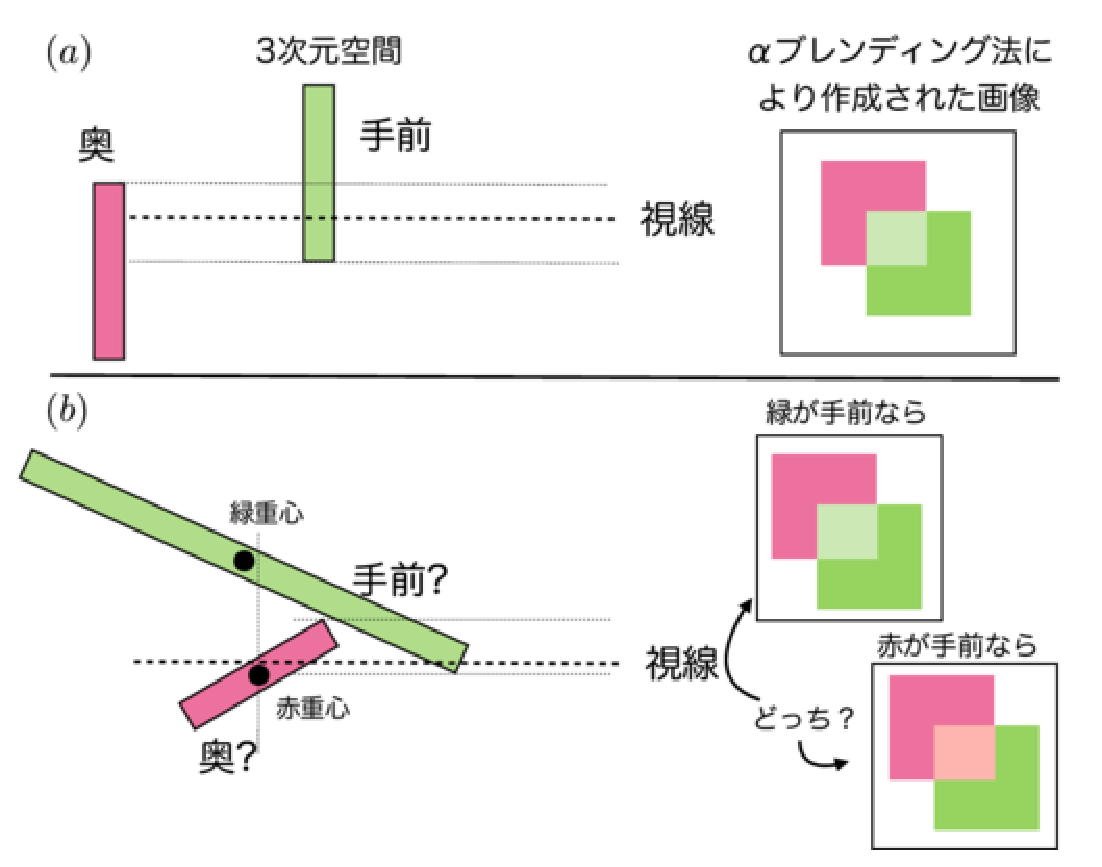
\includegraphics[width=70mm]{./Figures/eps/005.eps}
\end{wrapfigure}

図(a)では視線に対して,緑のオブジェクトが手前,赤が奥となっています.緑のオブジェクトを構成するどの頂点も,赤のオブジェクトを構成する頂点よりも手前にあることが計算できるので,自動的に奥行き判定をすることができ,$\alpha$ブレンディング法を実行できます.

一方(b)も同じ状況ですが,緑のオブジェクトを構成する頂点は,赤のオブジェクトを構成する頂点よりも手前,もしくは奥にあるため一概には判定できません.情報を減らして,それぞれの重心位置で比較することも考えられますが,この場合は「緑が奥にある」
と判定されてしまい,意図した結果となりません.

$\alpha$ブレンディング法を実行するために3次元オブジェクトの手前と奥を特徴づけるよい方法があれば良いのですが,筆者の調べた限りでは,そのような方法は無いようです.バージョン1.xのGLSC3Dでは,$\alpha$ブレンディング法における本問題はプログラマの責任で対処するしかなさそうです.

\subsubsection{物体の透明化における注意点(Ver1.x 以降 をお使いの方へ)}

しかしながら,これでは不便であるということでVer2.0からはある手続きを行うことで透明化処理を自動的に行わせることが可能となりました.(この処理を自動的に実行させるためには,GLSC3Dの初期化関数\verb|g_init_core|にて\verb|g_enable_transparent_out = 1|としてください.)ですので,以降の説明は必ずしも読む必要はありませんが,高度なプログラミングを行いたい方は知識として知っておいてください.

関数を基本的なアイデアは簡単で以下のような手続きを踏んでいます.
\begin{itemize}
\item ステップ1:任意の3次元オブジェクトを3角形分割する
\item ステップ2:3角形分割された描画命令を溜め込む
\item ステップ3:3角形の重心を求め,視点に対して遠い順番に並べ替え溜め込む
\item ステップ4:\verb|g_finish|が呼ばれた段階で,視点に対して遠い3角形から描画を行う
\end{itemize}

\noindent {\bf ステップ1:任意の3次元オブジェクトを3角形分割する}

任意の3次元オブジェクトは3角形分割によって描画することが可能です.分割数は多いほど滑らかな表示になります.GLSC3Dでは面を描く場合,内部の関数では最終的にはすべて\verb|g_triangle_3D_core|がCallされています.逆にユーザーが自身で関数を設計する場合も\verb|g_triangle_3D_core|を用いてプログラミングを行ってください.用いない場合は透明化処理が適切に自動化されません.

\noindent {\bf ステップ2:3角形分割された描画命令を溜め込む}

\verb|g_enable_transparent = 1|の場合,GLSC3Dは描画命令を溜め込むバッファ(以降\verb|TRIANGLE_BUFFER|と呼びます)を自動的に確保します.デフォルトの\verb|TRIANGLE_BUFFER|のサイズは$2^{20}$個の三角形を登録できるようなサイズ(大体500MBに相当)です.ほとんどこのサイズで問題は起きないはずですが,使用中too many triangles for triangle bufferなどと表示される場合は関数\verb|g_init_core|にてバッファサイズ(\verb|TRIANGLE_BUFFER_SIZE|)をさらに大きくしてください.

\noindent {\bf ステップ3:3角形の重心を求め,視点に対して遠い順番に並べ替え溜め込む}

3角形の重心を求めることは容易ですが,視点に対して遠い順番に並べ替える方法をどのように実装するかは難しい問題でした.GLSC3Dでは3角形の描画命令を\verb|TEMPORARY_TRIANGLE_BUFFER_SIZE|の数だけクイックソートアルゴリズムを用いてソートし,テンポラリなバッファ(以降\verb|TEMPORARY_TRIANGLE_BUFFER|と呼びます)にスタックします.その後,マージソートアルゴリズムを用いて\verb|TRIANGLE_BUFFER|にマージ&ソートし情報をアップデートします.このように\verb|TRIANGLE_BUFFER|は現時点の\verb|TRIANGLE_BUFFER|と\verb|TEMPORARY_TRIANGLE_BUFFER|から作られます.どのようなアルゴリズムを用いてソートを行うことが最も高速となるかは自明ではないため,様々なアルゴリズムを組み合わせて用いました.その結果,少なくとも筆者の環境ではこの方式が最も高速でした.デフォルトの設定では\verb|TEMPORARY_TRIANGLE_BUFFER|のサイズ\verb|TEMPORARY_TRIANGLE_BUFFER_SIZE|は$2^{10}$個の三角形を登録できるようなサイズです.このサイズが極端に大きかったり,小さかったりすると描画が非常に遅くなることが確認されています.ただし,ここでいうサイズの大きさの問題は,描画するべき対象に依った問題となりますので,最適値はわかりません\footnote{将来的には描画の時間を内部的に取得し,最適値を漸近的に求めるようにするかもしれません}.多くの場合,デフォルト値で問題は生じないと思われますが,描画遅いなどの問題が生じた場合は関数\verb|g_init_core|にて\verb|TEMPORARY_TRIANGLE_BUFFER_SIZE|を変更し最適値を見つけてください.

\noindent {\bf ステップ4:\verb|g_finish|が呼ばれた段階で,視点に対して遠い3角形から描画を行う}

ステップ3までの処理で,\verb|TRIANGLE_BUFFER|には視点から遠い順番で三角形の描画命令が登録されています.これらの三角形は\verb|g_finish|関数が呼ばれた時点で描画されます.

\vspace{10mm}
GLSC3DではGLSCと同様に標準座標系の中に複数の仮想座標系を構築することができますが,このステップ1$\sim$4は複数の仮想座標系において自動的に適用されます.したがって,{\bf ユーザーは\verb|g_triangle_3D_core|を用いて描画さえすれば,特に何も意識しなくても,正しく透明化処理を行うことができます}.ただし,透明化処理を行う際には別の注意も必要です.それは「3次元オブジェクトの三角形分割は十分に細かくなければならない」という点です.ステップ3において,3次元オブジェクトを大きな三角形で分割すると,分割が荒いことが影響し視点に対する奥行き判定の際に,ミスが生じます.このことを防ぐためには,3次元オブジェクトの三角形分割は十分に細かくする必要があります.例えば,\verb|g_sphere|という関数は与えられ点を中心に,与えられた半径の球を描画する関数です.この関数にはその上位関数として\verb|g_sphere_core|が存在しますが,その引数として\verb|int DivideLevel|があります.この\verb|DivideLevel|を$0$として指定する場合は1つの3角形を描きますが,$1$を指定すると4個の3角形,$2$を指定すると16個の3角形という具合に親3角形をさらに小さな子三角形へと分解し描画します.このような機能はほぼすべての描画関数に対して存在しますので,有効に活用してください.

透明化処理を行う際は,この点に注意いただくとともに,もし,さらに良いアイデアをお持ちの方がいましたら教えてください.

%%%%%%%%%%%%%%%%%%%%%%%%%%%%%%%%%%%%%%%%%%%%%%%%%%%%%%%%%%%%%%%%%%%%%%%%%%%
\newpage
\section{動作環境とその構築}
GLSC3D Ver. 3.0.0以降では,
依存ライブラリとインストール方法が変更されています.
必ずお読みください.

\subsection{動作環境}
GLSC3D Ver. 3.0.0以降では,OpenGL,SDL,libPNG,FreeType,Mathライブラリに依存します.
OpenGL,SDLはGLSC3Dの根幹部分です.
PNGライブラリは画面をキャプチャするために必要です\footnote{\url{http://www.libpng.org/pub/png/libpng.html}}.
C言語のMathライブラリは描画関数内で数学関数を用いているために必要です.
デフォルトの設定では,頂点データを保持用に,
概ね500KB+1048KBのメモリー領域を使用します.

%%多くの場合,MacOS\footnote{MacOSはUNIXと認められましたが...},
%%Linux,UNIX ではSDL以外は標準的にインストールされています.

\subsection{動作環境の構築}
GLSC3D Ver. 3.0.0以降では,
GLSC3DをインストールためのシェルスクリプトをOS毎に用意しています.
\url{http://www-mmc.es.hokudai.ac.jp/~masakazu/}の公開ソフトウェアから対応するスクリプトをダウンロードし,
実行することによってインストールが行われます.

\subsubsection{Mac OS Xの場合}

\noindent
{\bf (1) Xcodeのインストール:}

Mac OS XはXcodeを導入しなければ,様々な開発環境がインストールされません.
まずXcodeをインストールしてください.
App StoreでXcodeを検索すればトップに表示されます.

\noindent 
{\bf (2) Mac OS X用シェルスクリプト:} 

Script\_on\_mac.zipを解凍すると以下の実行ファイルが入手できます:
\begin{itemize}
\item[] 1\_Install\_macports\_mac
\item[] 2\_Install\_dependency\_library\_mac
\item[] 3\_Test\_GLSC3D\_on\_mac
\item[] 4\_Install\_GLSC3D\_on\_your\_mac
\end{itemize}

\begin{wrapfigure}{r}{50mm}
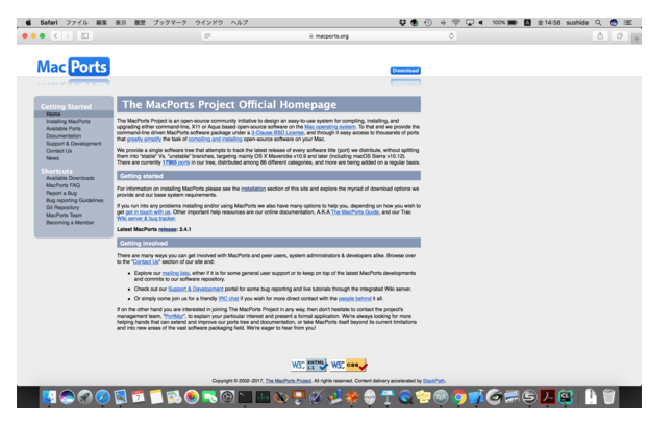
\includegraphics[width=50mm]{./Figures/eps/Canvas_macports.eps}
\vspace{-4\baselineskip}
\end{wrapfigure}

\noindent 
{\bf (3) 1\_Install\_macports\_macの実行:} 

1つ目のスクリプトでは,MacPortsがインストールされているかを確認します.
以下のように実行すると,右図のようにブラウザで\verb|https://www.macports.org/|のページが開くので,
インストールしていない場合はダウンロードおよびインストールを行って下さい.

\begin{itembox}[l]{スクリプトの実行}
\verb|$: ./1_Install_macports_mac|
\end{itembox}

無事にインストールされたら,次のステップに進んで下さい.

\noindent 
{\bf (4) 2\_Install\_dependency\_library\_macの実行:} 

2つ目のスクリプトでは,GLSC3Dが依存しているライブラリでMac OS Xに必要なもの
(cmake, libPNG, libsdl2)を導入します.

\begin{itembox}[l]{スクリプトの実行}
\verb|$: ./2_Install_dependency_library_mac|
\end{itembox}

無事にインストールされたら,次のステップに進んで下さい.

\noindent 
{\bf (5) 3\_Test\_GLSC3D\_on\_macの実行:} 

\begin{wrapfigure}{r}{60mm}
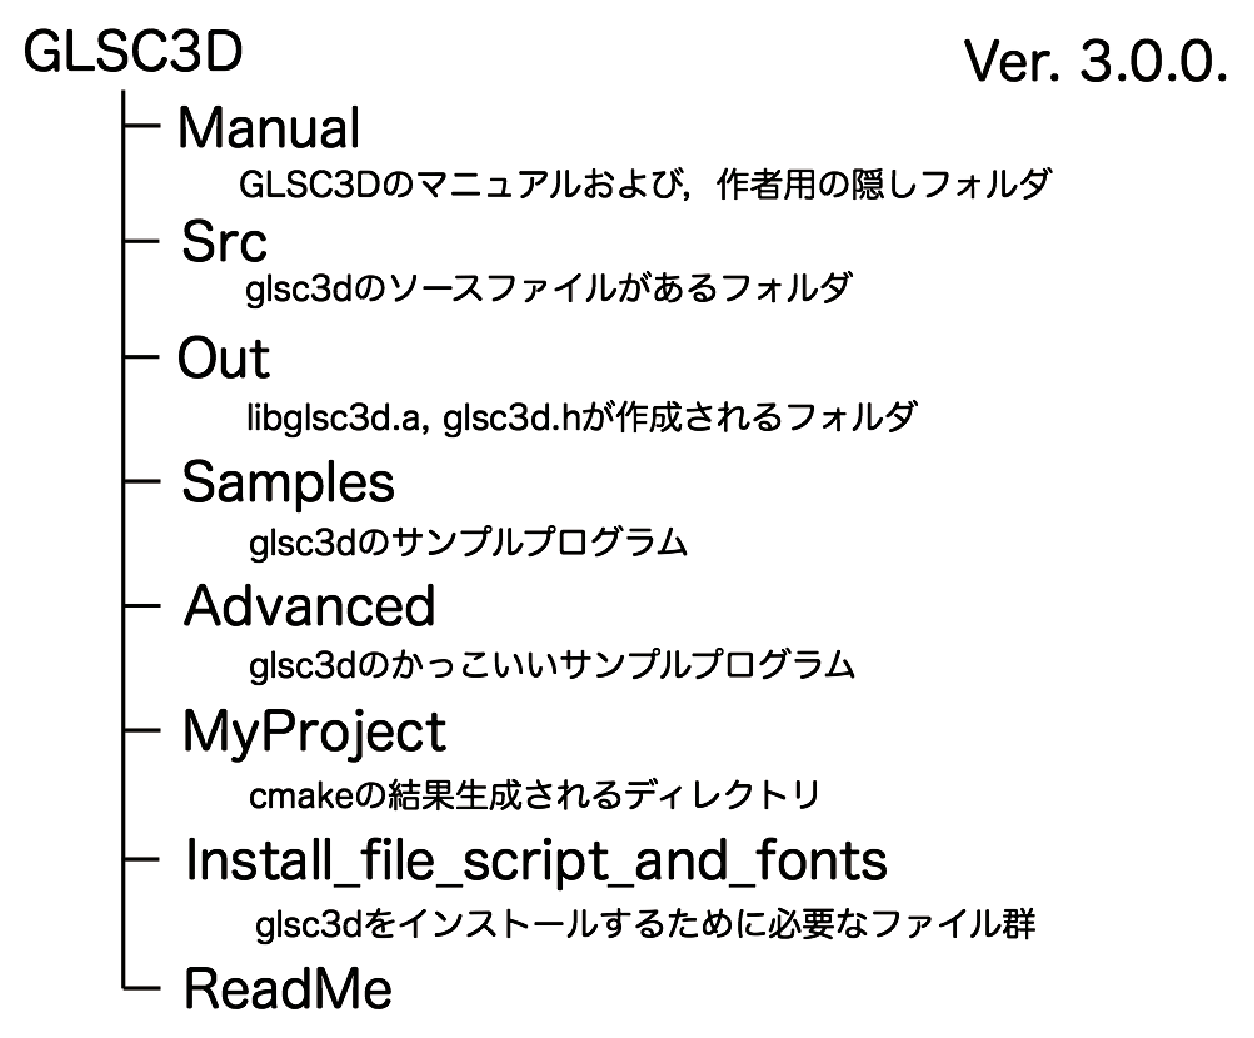
\includegraphics[width=60mm]{./Figures/eps/Canvas_Directory_GLSC3D.eps}
\end{wrapfigure}

3つ目のスクリプトでは,
はじめに\verb|$HOME|に\verb|GLSC3D_Working_Directory|というディレクトリが作成され,
\verb|GLSC3D_Working_Directory|に
\url{https://github.com/GLSC3DProject/GLSC3D}
から最新版のGLSC3Dがダウンロードされます.
\verb|GLSC3D_Working_Directory|内のファイルは下図のようになります.
また,フォントファイルがシステムにない場合は\verb|$HOME/Library/Fonts|にインストールされます.
次に,全てのサンプルプログラムとアドバンスドプログラムが実行できるかを確認します.
サンプルプログラムとアドバンスドプログラムは実行時間がすこしかかるので,Noを選択してスキップすることもできます.
各プログラムは\verb|esc|キーを押すと終了します.

\begin{itembox}[l]{スクリプトの実行}
\verb|$: ./3_Test_GLSC3D_on_mac|
\end{itembox}

\begin{figure}[htb]
\centering
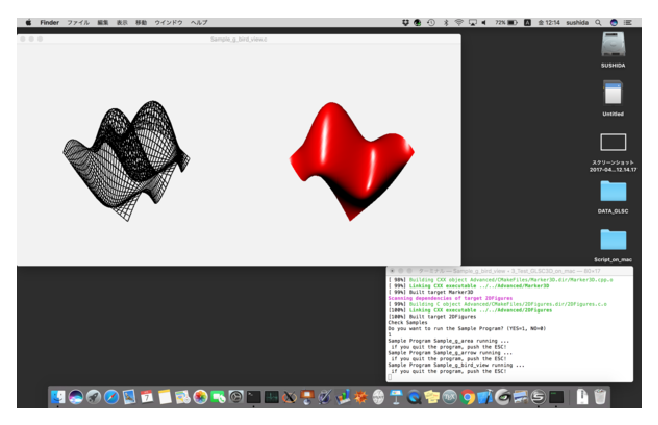
\includegraphics[scale=.6]{./Figures/eps/Canvas_Samples.eps}
\hspace{2zw}
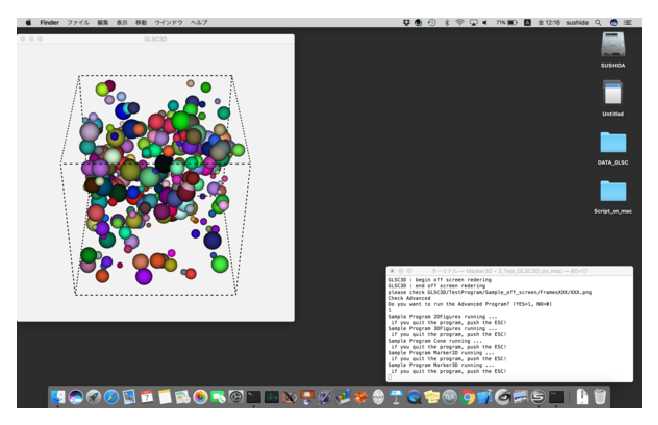
\includegraphics[scale=.6]{./Figures/eps/Canvas_Advanced.eps}
\end{figure}

無事にインストールされたら,次のステップに進んで下さい.

\noindent 
{\bf (6) 4\_Install\_GLSC3D\_on\_your\_macの実行:} 

4つ目のスクリプトでは,
はじめに\verb|$HOME|直下に3つのフォルダ\verb|bin|,\verb|include|,\verb|lib|を作成し,
\verb|ccg|を\verb|bin|に,
\verb|glsc3d.h|,\verb|glsc3d_math.h|を\verb|include|に,
\verb|libgslc3d.a|を\verb|lib|に,
\verb|Hello_GLSC3D.c|を\verb|GLSC3D_Working_Directory|の直下に保存します.
次に,
\verb|bin|,\verb|include|
にパスが通っているかの確認をします.

\begin{itembox}[l]{スクリプトの実行}
\verb|$: ./4_Install_GLSC3D_on_your_mac|
\end{itembox}

\begin{wrapfigure}{r}{60mm}
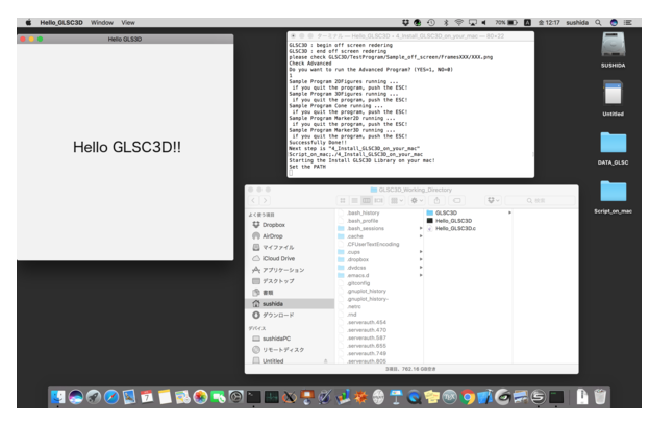
\includegraphics[width=60mm]{./Figures/eps/Canvas_Hello_GLSD3D.eps}
\vspace{-4\baselineskip}
\end{wrapfigure}

パスが通っていない場合はメッセージに従って,
下記のように使用しているシェル(.bashrc or .profileなど)を編集して下さい.

\begin{itembox}[l]{パスの通し方}
\verb|export PATH=$PATH:$HOME/bin|
	
\verb|export PATH=$PATH:$HOME/include|
\end{itembox}

無事にパスが通っていれば,
\verb|bin|内の\verb|ccg|コマンドによって自動的にサンプルプログラム \verb|Hello_GLSC3D.c| がコンパイルされ,実行されます.
(右図のように実行画面が表示されれば正しいです.)
実行がうまく行った場合は,システムに正しくGLSC3Dがインストールされたことになります.

%%%%%%%%%%%%%%%%%%%%%%%%%%%%%%%%%%%%%%%%%%%%%%%%%%%%%%%%%%%%%%%%%%%
\subsubsection{Ubuntuの場合}

\noindent 
{\bf (1) Ubuntu用シェルスクリプト:} 

Script\_on\_ubuntu.zipを解凍すると以下の実行ファイルが入手できます:
\begin{itemize}
\item[] 1\_Install\_dependency\_library\_ubuntu
\item[] 2\_Test\_GLSC3D\_on\_ubuntu
\item[] 3\_Install\_GLSC3D\_on\_your\_ubuntu
\end{itemize}

\noindent 
{\bf (2) 1\_Install\_dependency\_library\_ubuntuの実行:} 

1つ目のスクリプトでは,GLSC3Dが依存しているライブラリでUbuntuに必要なもの
(git, cmake, libPNG, libsdl2, freetype)を導入します.

\begin{itembox}[l]{スクリプトの実行}
\verb|$: ./2_Install_dependency_library_ubuntu|
\end{itembox}

無事にインストールされたら,次のステップに進んで下さい.

\noindent 
{\bf (3) 2\_Test\_GLSC3D\_on\_ubuntuの実行:} 

2つ目のスクリプトでは,
はじめに\verb|$HOME|に\verb|GLSC3D_Working_Directory|というディレクトリが作成され,
\verb|GLSC3D_Working_Directory|に
\url{https://github.com/GLSC3DProject/GLSC3D}
から最新版のGLSC3Dがダウンロードされます.
また,フォントファイルがシステムにない場合は\verb|/usr/share/fonts/opentype/noto|にインストールされます.
次に,全てのサンプルプログラムとアドバンスドプログラムが実行できるかを確認します.
サンプルプログラムとアドバンスドプログラムは実行時間がすこしかかるので,Noを選択してスキップすることもできます.
実行結果はMac OS Xと同様です.

\begin{itembox}[l]{スクリプトの実行}
\verb|$: ./2_Test_GLSC3D_on_ubuntu|
\end{itembox}

無事にインストールされたら,次のステップに進んで下さい.

\noindent 
{\bf (4) 3\_Install\_GLSC3D\_on\_your\_ubuntuの実行:} 

4つ目のスクリプトでは,
はじめに\verb|$HOME|直下に3つのフォルダ\verb|bin|,\verb|include|,\verb|lib|を作成し,
\verb|ccg|を\verb|bin|に,
\verb|glsc3d.h|,\verb|glsc3d_math.h|を\verb|include|に,
\verb|libgslc3d.a|を\verb|lib|に,
\verb|Hello_GLSC3D.c|を\verb|GLSC3D_Working_Directory|の直下に保存します.
次に,
\verb|bin|,\verb|include|
にパスが通っているかの確認をします.

\begin{itembox}[l]{スクリプトの実行}
\verb|$: ./3_Install_GLSC3D_on_your_ubuntu|
\end{itembox}

パスが通っていない場合はメッセージに従って,
下記のようにシェルを編集して下さい.

\begin{itembox}[l]{パスの通し方: 使用しているシェル(.bashrc or .profileなど)において書きを追加します.}
\verb|export PATH=$PATH:$HOME/bin|
	
\verb|export PATH=$PATH:$HOME/include|
\end{itembox}

無事にパスが通っていれば,
\verb|bin|内の\verb|ccg|コマンドによって自動的にサンプルプログラム \verb|Hello_GLSC3D.c| がコンパイルされ,実行されます.
実行結果はMac OS Xと同様です.
実行がうまく行った場合は,システムに正しくGLSC3Dがインストールされたことになります.

%%%%%%%%%%%%%%%%%%%%%%%%%%%%%%%%%%%%%%%%%%%%%%%%%%%%%%%%%%%%%%%%%%%%%%%%%%%
\subsubsection{CentOSの場合}

CentOSでのインストールでは,
glxinfoにてOpenGLのバージョンが4.1以降であることと
libpngおよびfontに対するパスの指定が正しくできていれば動作する可能性があります.
ライブラリのバージョンがUbuntuに比べて古いので動作の保証ができません.
GLSC3D Ver. 2.1.1を使用されることをお勧めします.


%%%%%%%%%%%%%%%%%%%%%%%%%%%%%%%%%%%%%%%%%%%%%%%%%%%%%%%%%%%%%%%%%%%%%%%%%%%
\subsubsection{Windowsの場合}

Windowsを使用する場合,Visual Studio 2017を使ってください.Visual Studio 2017ではCMakeがサポートされています.
Community Editionは無料で使用することができます.
インストールの際はC++によるデスクトップ開発にチェックを入れてください.

%%%%%%%%%%%%%%%%%%%%%%%%%%%%%%%%%%%%%%%%%%%%%%%%%%%%%%%%%%%%%%%%%%%%%%%%%%%
%%\newpage
%%\section{GLSC3Dのインストールとテスト}
%%
%%GLSC3Dは一般的なソフトウェアと同じように,ライブラリ(\verb|libglsc3d.a|, \verb|libglsc3d.dylib|, \verb|libglsc3d.so|(linuxのみ))とヘッダーファイル(\verb|glsc3d.h|)の2つで提供されます.そこで,本章ではこれらのファイルの作成方法とインストールの方法に関して説明します.
%%
%%\begin{wrapfigure}[11]{r}{70mm}
%%\vspace{-1\baselineskip}
%%	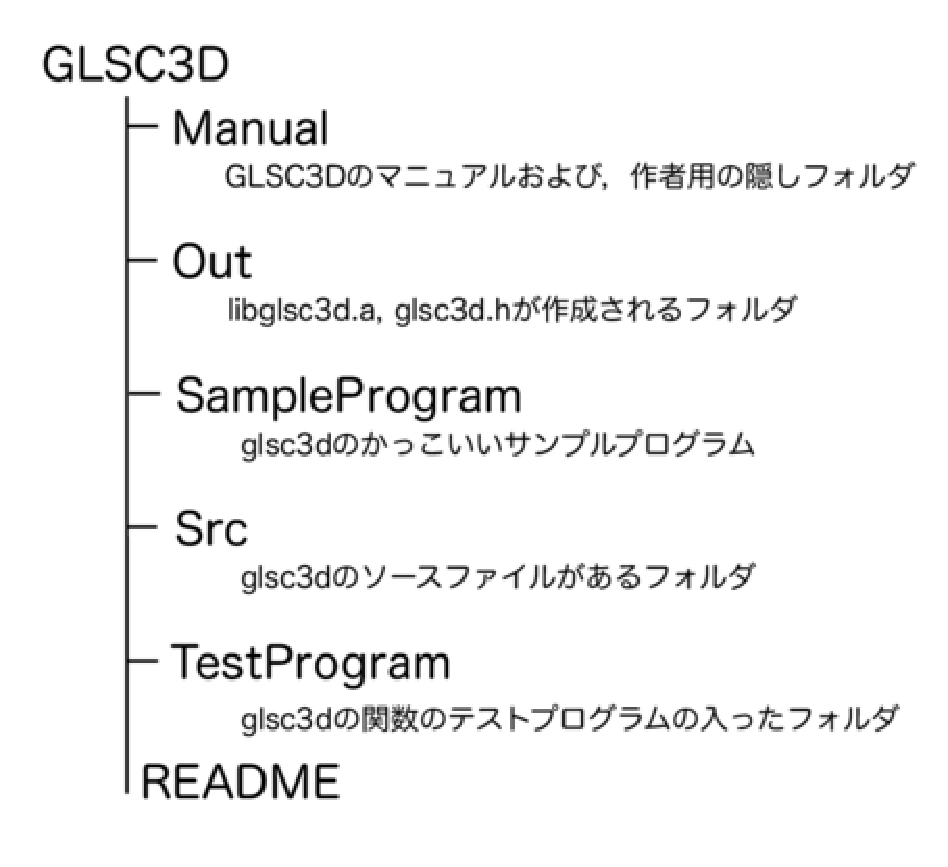
\includegraphics[width=70mm]{./Figures/eps/006.eps}
%%\end{wrapfigure}
%%
%%GLSC3D.zipをデスクトップに展開してください.GLSC3Dの構成は右のようになっているはずです.ここからはターミナルでの操作となります.Srcフォルダに移動し,makeを実行してください.すなわち,
%%
%%\verb|$: cd Src|
%%
%%\verb|$: make|
%%
%%\noindent
%%としてください.様々なファイルがコンパイルされOutフォルダにライブラリ(\verb|libglsc3d.a|, \verb|libglsc3d.dylib|, \verb|libglsc3d.so|(linuxのみ))とヘッダーファイル(\verb|glsc3d.h|)が作成されます.もし,作成されない場合は\verb|/usr/X11R6/lib|にOpenGL,GLUT,PNGライブラリが,\verb|/usr/X11R6/include|にそれらのヘッダーファイルがそれぞれ置かれていないことが原因です.適切な場所に置くか,Makefileを書き換えてください.筆者はMacOS, Ubuntu, CentOSなどの環境で問題なく作成されることを確認しています.
%%
%%\begin{wrapfigure}[11]{r}{70mm}
%%\vspace{-1\baselineskip}
%%	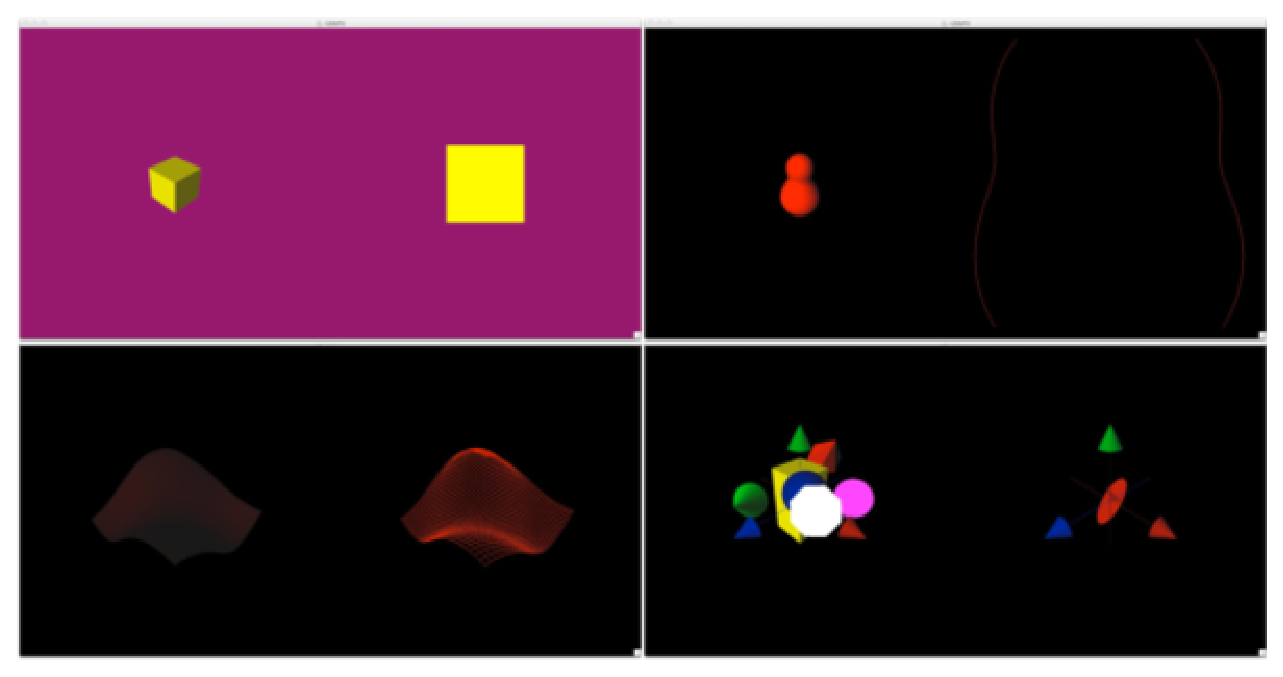
\includegraphics[width=70mm]{./Figures/eps/007.eps}
%%\end{wrapfigure}
%%
%%作られたライブラリとヘッダーファイルが正常に動作すること確認するために,SampleProgramフォルダ下のusing\_makefileフォルダに移動してください.そしてmakeを実行してください.test\_programという実行ファイルが作られるので,実行してください.すなわち,
%%
%%\verb|$: cd ../SampleProgram/using_makefile|
%%
%%\verb|$: make|
%%
%%\verb|$: ./Run|
%%
%%\noindent
%%としてください.GLSC3Dのデモプログラムが実行されます.
%%
%%Linuxの場合は
%%
%%\verb|$: ./Run_linux|
%%
%%\noindent
%%としてください.GLSC3Dのデモプログラムが実行されます.
%%
%%\verb|SampleProgram/using_glsc3dcommand|では,Makeコマンドを使用せずにデモプログラムを実行できます.その際,GLSC3D用のコマンド\verb|ccg|を用いています.どちらの場合でも正常にデモプログラムが実行されているかを確認して下さい.確認がとれたらライブラリ(\verb|libglsc3d.a|, \verb|libglsc3d.dylib|, \verb|libglsc3d.so|(linuxのみ))とヘッダーファイル(\verb|glsc3d.h|)とヘッダーファイル(\verb|glsc3d.h|)を適切な場所へコピーします.筆者は自身のhomeディレクトリの下にlibと,includeフォルダを作成し,それぞれのファイルを置くことを推奨します.
%%そこでライブラリが作られたことを確認した後に以下のように打ってください.
%%
%%\verb|$: make install |
%%
%%これは
%%
%%\verb|$: cp Out/libglsc3d.a Out/libglsc3d.dylib ~/lib/| (macの場合)
%%
%%\verb|$: cp Out/libglsc3d.a Out/libglsc3d.so ~/lib/| (linuxの場合)
%%
%%\verb|$: cp Out/glsc3d.h ~/include/|
%%
%%と同じ意味です.
%%
%%suの権限を持つならば,/usr/libや/usr/include下のようなパスの通ったフォルダに置いてもいいでしょう.
%%
%%そこでライブラリが作られたことを確認した後に以下のように打ってください.
%%
%%\verb|$: make install_root |
%%
%%これは
%%
%%\verb|$: sudo cp Out/libglsc3d.a Out/libglsc3d.dylib /usr/lib/| (macの場合)
%%
%%\verb|$: sudo cp Out/libglsc3d.a Out/libglsc3d.so /usr/lib/| (linuxの場合)
%%
%%\verb|$: sudo cp Out/glsc3d.h /usr/include/|
%%
%%と同じ意味です.
%%
%%これにてインストールは完了です.

%%%%%%%%%%%%%%%%%%%%%%%%%%%%%%%%%%%%%%%%%%%%%%%%%%%%%%%%%%%%%%%%%%%%%%%%%%%
\newpage
\section{GLSC3Dの関数}
%\begin{wrapfigure}{r}{70mm}
%\vspace{-1\baselineskip}
%	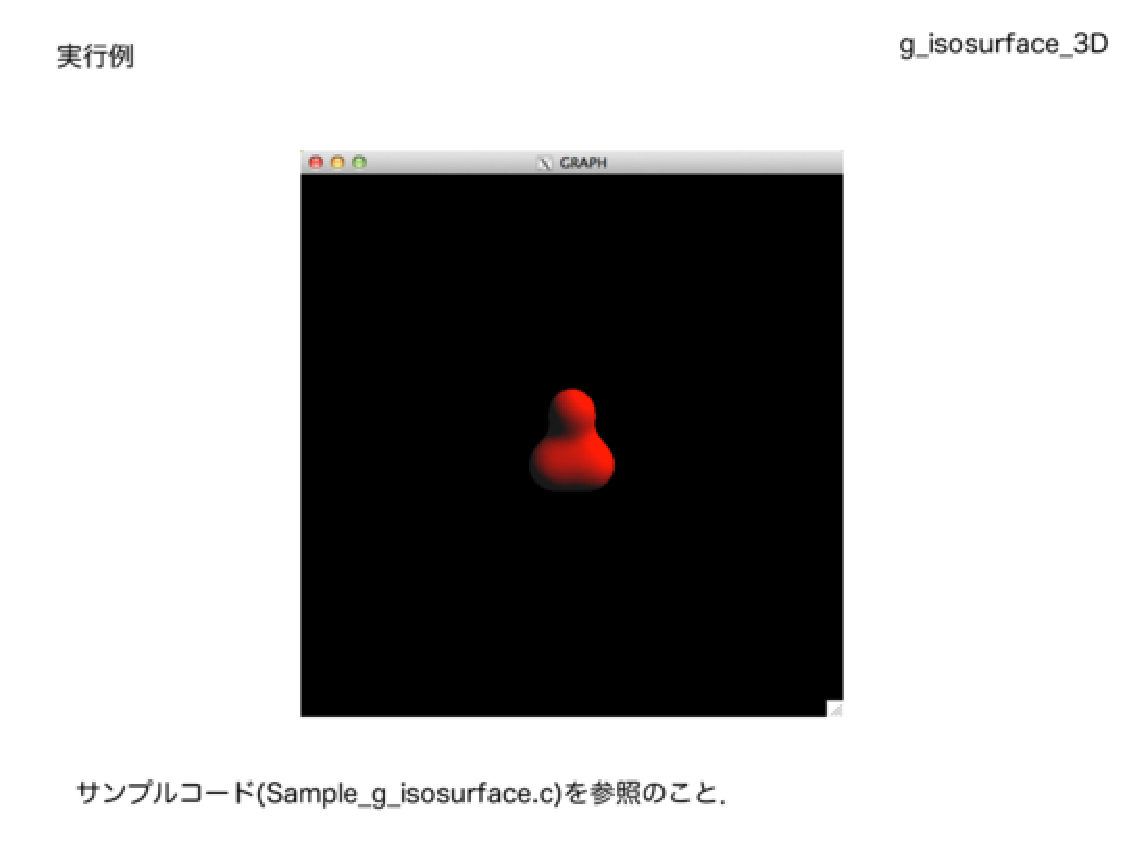
\includegraphics[width=70mm]{./Figures/eps/GLSC3D_Manual-94.eps}
%\end{wrapfigure}

GLSC3DはGLSCと同様に一枚のキャンバスに対して,いくつかの絵を描画するようなソフトであると考えてください.適切な関数を用い,キャンバスをいくつかのエリアに区切り,それぞれのエリアに描きたいもの(3次元,2次元,テキスト等)を描画することができます.
\begin{figure}[htb]
\centering
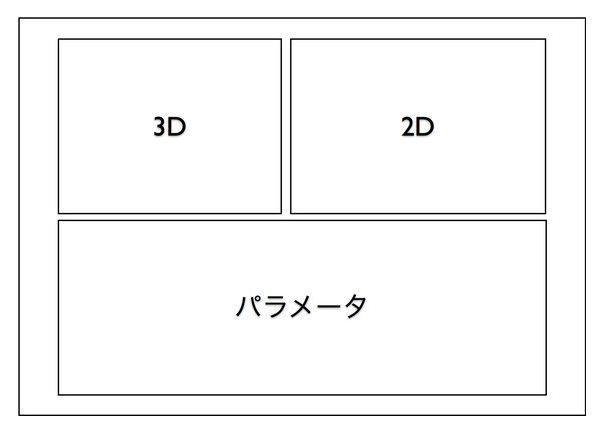
\includegraphics[width=100mm]{./Figures/eps/Canvas_kansu_gaiyo.eps}
\end{figure}

GLSC3Dを利用する際,多くの場合基本的な枠組みは以下のような形態となるでしょう.ここでは我々が用意した関数それぞれについての説明とその実行例も記載しておりますので,個々の関数の使用方法はそちらをご覧ください.なお,具体的な使用例はサンプルプログラムがありますので,そちらをご覧ください.\\

\newpage
基本的な枠組み
\begin{verbatim}
#include <...>
...
#include <glsc3d.h>

int main()
{
    g_init(...);						//用紙の設定
    g_def_scale_3D(0,...);			//0番の仮想座標系の定義
    g_def_scale_3D(1,...);			//1番の仮想座標系の定義
    ...
        
/****************************************/	
                数値計算
/****************************************/

    g_cls();						//用紙を背景色で塗りつぶす
   
    //仮想座標系を選択→属性を指定→描画関数で描画.
    g_sel_scale_3D(0);			//0番の仮想座標系を選択(以下,0番の仮想座標系に描かれる.)	
    g_area_color_3D(...);			//塗りつぶしの色を指定
    g_box_3D(...);				//3次元空間にboxを描画
    ...
    
    //仮想座標系を選択→属性を指定→描画関数で描画.
    g_sel_scale_3D(1);			//1番の仮想座標系を選択(以下,1番の仮想座標系に描かれる.)
    g_area_color_3D(...);			//塗りつぶしの色を指定
    g_sphere_3D(...);				//3次元空間にsphereを描画
    ...
           
    g_finish();					//描画する
    return 0;
}

\end{verbatim}
用語の解説\\
\noindent
・標準座標系:標準座標系とは,ディスプレイ左上を(0.0,0.0)とするピクセル単位の座標系のこと.

\noindent
・仮想座標系:仮想座標系とは,\verb|g_def_scale|で定義する座標系のこと.
先の例で言えばキャンバスは標準座標系,さらにキャンバス内のあるエリアは仮想座標系となります.GLSC3Dでははいくつかの例外を除いて描画は仮想座標系に対して行われます.(例外:\verb|g_text_standard|).

\noindent
・属性:例えば線を描く場合,色や線の太さなどを指定したいこともあります.色や線の太さなどを属性と呼び,属性を適切に設定することで,描きたい描画対象の属性を変更し描くことが出来ます.この属性は属性コントロール関数を用いて変化させることができます.

\vspace{5mm}
\noindent
関数名について

\noindent
・``\verb|_2D|"や``\verb|_3D|"がついていないもの・・・2次元描画と3次元描画で共に使用可能.

\noindent
・``\verb|_2D|"がついてるもの・・・2次元描画のみで使用可能,もしくは,3次元描画で使用すると描画が不自然となるもの.

\noindent
・``\verb|_3D|"がついてるもの・・・3次元描画のみで使用可能,もしくは,2次元描画で使用すると描画が不自然となるもの.

%\begin{figure}[htb]
%\vspace{-1\baselineskip}
%	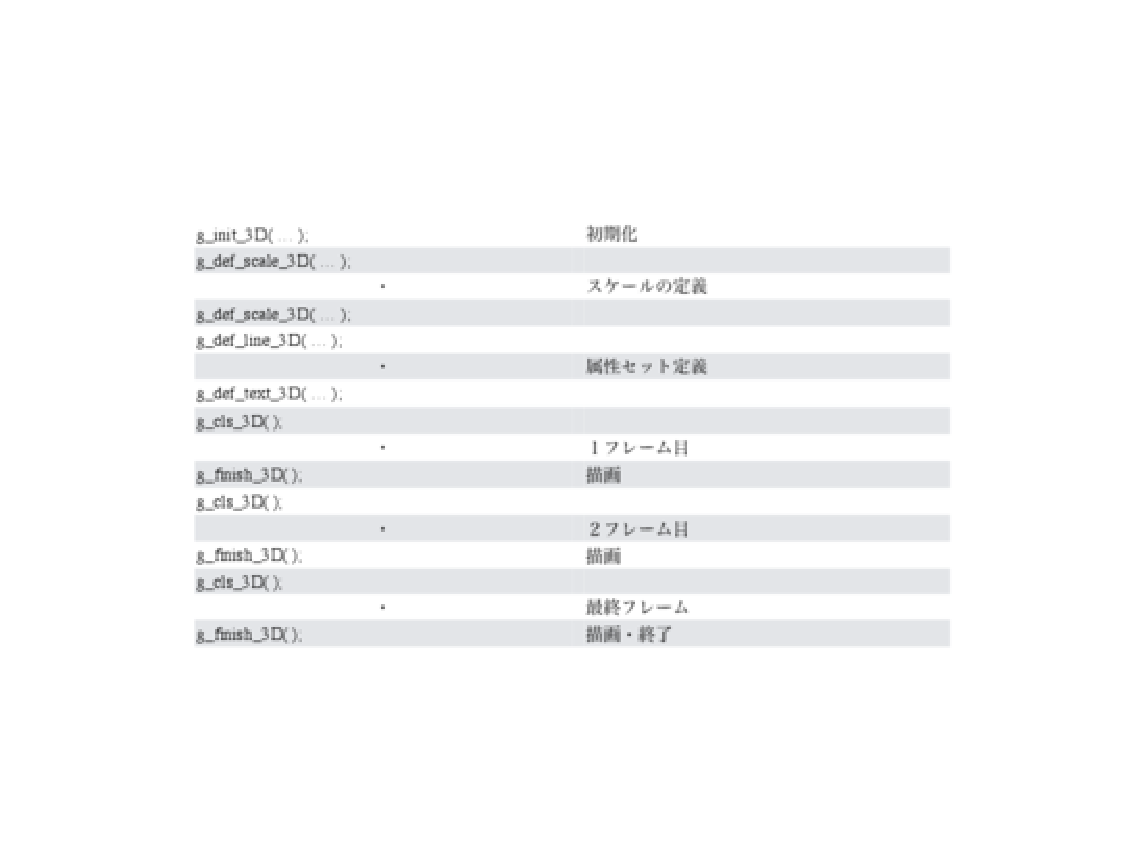
\includegraphics[width=140mm]{./Figures/eps/GLSC3D_Manual-2.eps}
%\end{figure}

%新関数の使用方法などに関しては付録.pdfを参考にしてください.

\clearpage
\subsection{制御関数}

%%%%%%%%%%%%%%%%%%%%%g_init%%%%%%%%%%%%%%%%%%%%%%%%%%%%%%
\subsubsection{\texttt{g\_init}}

\begin{itembox}[l]{\texttt{g\_init}関数}
%%%%%%%%%%%%%%%%%%%ここにプロトタイプ宣言を書く%%%%%%%%%%%%%%%%%%%
\begin{verbatim}
void g_init(
        const char *WindowName,
        int width, int height);
\end{verbatim}
%%%%%%%%%%%%%%%%%%%ここに引数の説明を書く%%%%%%%%%%%%%%%%%%%%%%%
\verb|WindowName| ; ウィンドウの名前,又は\verb|G_OFF_SCREEN|を設定します.\verb|G_OFF_SCREEN|では画面は表示されません\\
\verb|width| ; ウィンドウの幅(ディスプレイ上の座標(ピクセル単位))\\
\verb|height| ; ウィンドウの高さ( ディスプレイ上の座標(ピクセル単位))
\end{itembox}

%%%%%%%%%%%%%%%%%%%ここに関数の説明を書く%%%%%%%%%%%%%%%%%%%%%%%
\begin{itembox}[l]{\texttt{g\_init}関数の説明}
描画するウィンドウを設定するための関数です.ウィンドウはディスプレイの中央に表示されます.
\verb|G_OFF_SCREEN|を設定した場合,画面は表示されませんが,キャプチャーは問題なく行えます.
※当然ながら,マウス・キーボードを用いたインタラクティブな操作は出来なくなります.
\end{itembox}

%%%%%%%%%%%%%%%%%%%ここに関数の説明に使う絵を載せる.%%%%%%%%%%%%%%%%
%\begin{figure}[htb]
%	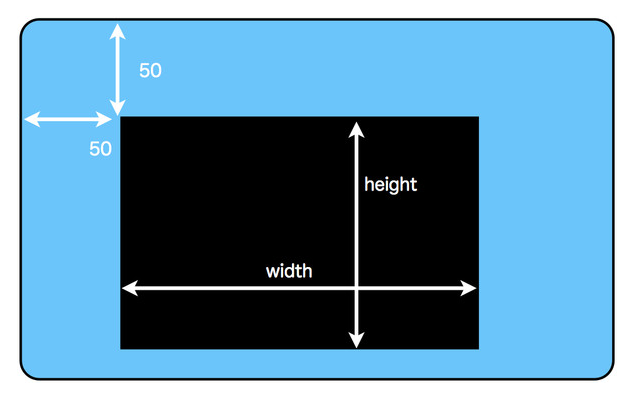
\includegraphics[width=100mm]{./Figures/eps/Canvas_g_init.eps}
%\end{figure}
%%%%%%%%%%%%%%%%%%%%%%%%%%%%%%%%%%%%%%%%%%%%%%%%%%%%%%

%%%%%%%%%%%%%%%%%%%%%g_init_core%%%%%%%%%%%%%%%%%%%%%%%%%%%
\clearpage
\subsubsection{\texttt{g\_init\_core}}

\begin{itembox}[l]{\texttt{g\_init\_core}関数}
%%%%%%%%%%%%%%%%%%%ここにプロトタイプ宣言を書く%%%%%%%%%%%%%%%%%%%
\begin{verbatim}
void g_init_core(
        const char *WindowName,
        int width, int height,
        int pos_x, int pos_y,
        float r, float g, float b,
        int enable_transparent,
        int temporary_triangle_buffer_size, 
        int triangle_buffer_size);
\end{verbatim}
%%%%%%%%%%%%%%%%%%%ここに引数の説明を書く%%%%%%%%%%%%%%%%%%%%%%%
\verb|WindowName| ; ウィンドウの名前,又は\verb|G_OFF_SCREEN|を設定します.\verb|G_OFF_SCREEN|では画面は表示されません\\
\verb|width| ; ウィンドウの幅(ピクセル単位)\\
\verb|height| ; ウィンドウの高さ(ピクセル単位)\\
\verb|pos_x| ; ウィンドウの左上x座標(ピクセル単位)または \verb|G_WINDOW_CENTERED|\\
\verb|pos_y| ; ウィンドウの左上y座標(ピクセル単位)または \verb|G_WINDOW_CENTERED|\\
\verb|r, g, b| ; 背景色の初期値を設定(不透明度は1に固定)\\
\verb|enable_transparent| ; 透明化処理にて並び替え機能を使用するか(1)しないか(0).\\
\verb|temporary_triangle_buffer_size| ;\\ 透明化処理用の\verb|TEMPORARY_TRIANGLE_BUFFER_SIZE|を指定する.デフォルトは$2^{10}$\\
\verb|triangle_buffer_size| ; 透明化処理用の\verb|TRIANGLE_BUFFER_SIZE|を指定する.デフォルトは$2^{20}$
\end{itembox}

%%%%%%%%%%%%%%%%%%%ここに関数の説明を書く%%%%%%%%%%%%%%%%%%%%%%%
\begin{itembox}[l]{\texttt{g\_init\_core}関数の説明}
描画するウィンドウを設定するための関数です.\texttt{g\_init}に比べて細かい制御が可能です.

Since Ver 3.0: \verb|pos_x, pos_y|に\verb|G_WINDOW_CENTERED|を指定すると,ウインドウをディスプレイの中央に表示します.
\end{itembox}

%%%%%%%%%%%%%%%%%%%ここに関数の説明に使う絵を載せる.%%%%%%%%%%%%%%%%
\begin{figure}[htb]
\centering
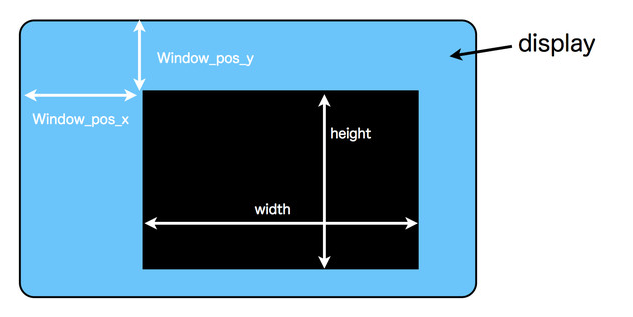
\includegraphics[width=100mm]{./Figures/eps/Canvas_g_init_core.eps}
\end{figure}
%%%%%%%%%%%%%%%%%%%%%%%%%%%%%%%%%%%%%%%%%%%%%%%%%%%%%%


\clearpage
%%%%%%%%%%%%%%%%%%%%%g_init_light%%%%%%%%%%%%%%%%%%%%%%%%%%%
\subsubsection{\texttt{g\_init\_light}}

\begin{itembox}[l]{\texttt{g\_init\_light}関数}
%%%%%%%%%%%%%%%%%%%ここにプロトタイプ宣言を書く%%%%%%%%%%%%%%%%%%%
\begin{verbatim}
void g_init_light(
        int lightnum,
        float x, float y, float z);
\end{verbatim}
%%%%%%%%%%%%%%%%%%%ここに引数の説明を書く%%%%%%%%%%%%%%%%%%%%%%%
\verb|lightnum| ; ライトの番号(0〜2)\\
\verb|x, y, z| ; ライトの方向座標
\end{itembox}

%%%%%%%%%%%%%%%%%%%ここに関数の説明を書く%%%%%%%%%%%%%%%%%%%%%%%
\begin{itembox}[l]{\texttt{g\_init\_light}関数の説明}
ライトの方向を設定するための関数です.ライトは常に平行光源です.ライト0から2の3個までの光源を設定できます.
この関数を呼ばずに描画した場合,デフォルト値として\texttt{g\_init\_light(0,1,1,1)}の光源が設定されます.
\end{itembox}

%%%%%%%%%%%%%%%%%%%%%g_init_light_core%%%%%%%%%%%%%%%%%%%%%%%%%%%
\subsubsection{\texttt{g\_init\_light\_core}}

\begin{itembox}[l]{\texttt{g\_init\_light\_core}関数}
%%%%%%%%%%%%%%%%%%%ここにプロトタイプ宣言を書く%%%%%%%%%%%%%%%%%%%
\begin{verbatim}
void g_init_light_core(
        int lightnum,
        float x, float y, float z, float power);
\end{verbatim}
%%%%%%%%%%%%%%%%%%%ここに引数の説明を書く%%%%%%%%%%%%%%%%%%%%%%%
\verb|lightnum| ; ライトの番号(0〜2)\\
\verb|x, y, z| ; ライトの方向座標\\
\verb|power| ; ライトの強さ
\end{itembox}

%%%%%%%%%%%%%%%%%%%ここに関数の説明を書く%%%%%%%%%%%%%%%%%%%%%%%
\begin{itembox}[l]{\texttt{g\_init\_light\_core}関数の説明}
\texttt{g\_init\_light}とほぼ同じですが,光源の強さを指定できます.
\end{itembox}

%%%%%%%%%%%%%%%%%%%%%g_disable_light%%%%%%%%%%%%%%%%%%%%%%%%%%%
\subsubsection{\texttt{g\_disable\_light}}

%%%%%%%%%%%%%%%%%%%ここに関数の説明を書く%%%%%%%%%%%%%%%%%%%%%%%
\begin{itembox}[l]{\texttt{g\_disable\_light}関数}
%%%%%%%%%%%%%%%%%%%ここにプロトタイプ宣言を書く%%%%%%%%%%%%%%%%%%%
\begin{verbatim}
void g_disable_light(
        int lightnum);
\end{verbatim}
%%%%%%%%%%%%%%%%%%%ここに引数の説明を書く%%%%%%%%%%%%%%%%%%%%%%%
\verb|lightnum| ; ライトの番号(0〜2)
\end{itembox}

%%%%%%%%%%%%%%%%%%%ここに関数の説明を書く%%%%%%%%%%%%%%%%%%%%%%%
\begin{itembox}[l]{\texttt{g\_disable\_light}関数の説明}
\verb|g_init_light, g_init_light_core|によって有効化されたライトを無効化します.
\end{itembox}


\clearpage
%%%%%%%%%%%%%%%%%%%%%g_scr_color%%%%%%%%%%%%%%%%%%%%%%%%%%%
\subsubsection{\texttt{g\_scr\_color}}

\begin{itembox}[l]{\texttt{g\_scr\_color}関数}
%%%%%%%%%%%%%%%%%%%ここにプロトタイプ宣言を書く%%%%%%%%%%%%%%%%%%%
\begin{verbatim}
void g_scr_color(
        float r, float g, float b, float a);
\end{verbatim}
%%%%%%%%%%%%%%%%%%%ここに引数の説明を書く%%%%%%%%%%%%%%%%%%%%%%%
\verb|r,g,b,a| ; 光の三原色+不透明度($0\leq \verb|r,g,b,a| \leq 1$)
\end{itembox}

%%%%%%%%%%%%%%%%%%%ここに関数の説明を書く%%%%%%%%%%%%%%%%%%%%%%%
\begin{itembox}[l]{\texttt{g\_scr\_color}関数の説明}
	背景色を設定するための関数です.
\end{itembox}

%%%%%%%%%%%%%%%%%%%ここに関数の説明に使う絵を載せる.%%%%%%%%%%%%%%%%
\begin{figure}[htb]
\centering
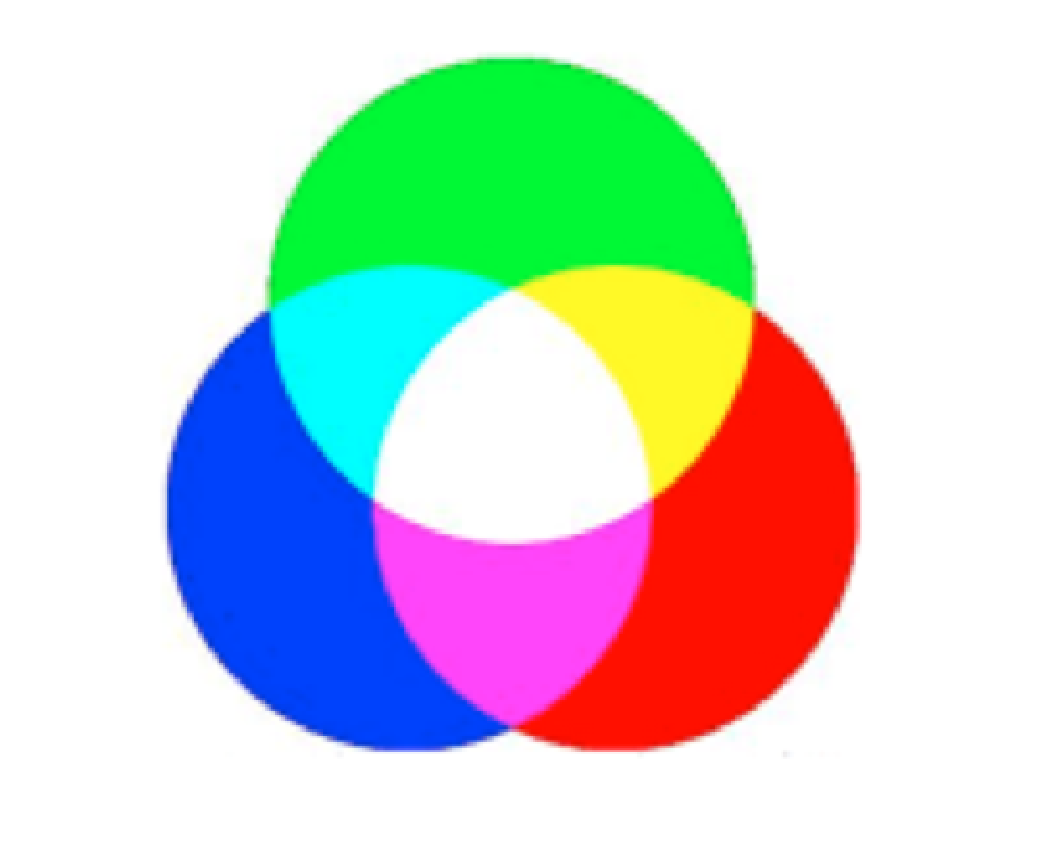
\includegraphics[width=100mm]{./Figures/eps/Canvas_g_scr_color.eps}
\end{figure}
%%%%%%%%%%%%%%%%%%%%%%%%%%%%%%%%%%%%%%%%%%%%%%%%%%%%%%


%%%%%%%%%%%%%%%%%%%%g_cls%%%%%%%%%%%%%%%%%%%%%%%%%%%%%%%

\subsubsection{\texttt{g\_cls}}

\begin{itembox}[l]{\texttt{g\_cls}関数}
%%%%%%%%%%%%%%%%%%%ここにプロトタイプ宣言を書く%%%%%%%%%%%%%%%%%%%
\begin{verbatim}
void g_cls();
\end{verbatim}
%%%%%%%%%%%%%%%%%%%ここに引数の説明を書く%%%%%%%%%%%%%%%%%%%%%%%
\end{itembox}

%%%%%%%%%%%%%%%%%%%ここに関数の説明を書く%%%%%%%%%%%%%%%%%%%%%%%
\begin{itembox}[l]{\texttt{g\_ cls}関数の説明}
	新しいフレームを背景色で塗りつぶす.
\end{itembox}


\clearpage
%%%%%%%%%%%%%%%%%%%%g_finish%%%%%%%%%%%%%%%%%%%%%%%%%%%%%%%
\subsubsection{\texttt{g\_finish}}

\begin{itembox}[l]{\texttt{g\_finish}関数}
%%%%%%%%%%%%%%%%%%%ここにプロトタイプ宣言を書く%%%%%%%%%%%%%%%%%%%
\begin{verbatim}
void g_finish();
\end{verbatim}
%%%%%%%%%%%%%%%%%%%ここに引数の説明を書く%%%%%%%%%%%%%%%%%%%%%%%
\end{itembox}

%%%%%%%%%%%%%%%%%%%ここに関数の説明を書く%%%%%%%%%%%%%%%%%%%%%%%
\begin{itembox}[l]{\texttt{g\_ finish}関数の説明}
この関数を呼ぶことで描画することができます.
\end{itembox}


%%%%%%%%%%%%%%%%%%%%g_sleep%%%%%%%%%%%%%%%%%%%%%%%%%%%%%%%
\subsubsection{\texttt{g\_sleep}}

\begin{itembox}[l]{\texttt{g\_sleep}関数}
%%%%%%%%%%%%%%%%%%%ここにプロトタイプ宣言を書く%%%%%%%%%%%%%%%%%%%
\begin{verbatim}
void g_sleep(
        double wait_time);
\end{verbatim}
%%%%%%%%%%%%%%%%%%%ここに引数の説明を書く%%%%%%%%%%%%%%%%%%%%%%%
\verb|wait_time| ; 静止時間(秒)
\end{itembox}

%%%%%%%%%%%%%%%%%%%ここに関数の説明を書く%%%%%%%%%%%%%%%%%%%%%%%
\begin{itembox}[l]{\texttt{g\_ sleep}関数の説明}
指定した秒数だけ静止します.
\end{itembox}

%%%%%%%%%%%%%%%%%%%ここに関数の説明に使う絵を載せる.%%%%%%%%%%%%%%%%
%%%%%%%%%%%%%%%%%%%%%%%%%%%%%%%%%%%%%%%%%%%%%%%%%%%%%%



%%%%%%%%%%%%%%%%%%%%g_capture, g_capture_set%%%%%%%%%%%%%%%%%%%%%%%%%%%%%%
\subsubsection{\texttt{g\_capture\_set, g\_capture}}

\begin{itembox}[l]{\texttt{g\_capture\_set, g\_capture}関数}
%%%%%%%%%%%%%%%%%%%ここにプロトタイプ宣言を書く%%%%%%%%%%%%%%%%%%%
\begin{verbatim}
void g_capture_set(
        const char *name);
void g_capture();
\end{verbatim}
%%%%%%%%%%%%%%%%%%%ここに引数の説明を書く%%%%%%%%%%%%%%%%%%%%%%%
\verb|name| ; 保存先のフォルダ名(``''または\verb|NULL|の場合,フォルダ名は「Frames年.月.日.時.分.秒」となる.)
\end{itembox}

%%%%%%%%%%%%%%%%%%%ここに関数の説明を書く%%%%%%%%%%%%%%%%%%%%%%%
\begin{itembox}[l]{\texttt{g\_capture\_set,g\_capture}関数の説明}
画面を取り込むための準備を行う関数.(\verb|g_capture_set|)

画面を取り込む関数.(\verb|g_capture|)
\end{itembox}

\clearpage
%%%%%%%%%%%%%%%%%%%%%g_enable_highdpi%%%%%%%%%%%%%%%%%%%%%%%%%%%
\subsubsection{\texttt{g\_enable\_highdpi}}

%%%%%%%%%%%%%%%%%%%ここに関数の説明を書く%%%%%%%%%%%%%%%%%%%%%%%
\begin{itembox}[l]{\texttt{g\_enable\_highdpi}関数}
%%%%%%%%%%%%%%%%%%%ここにプロトタイプ宣言を書く%%%%%%%%%%%%%%%%%%%
\begin{verbatim}
void g_enable_highdpi();
\end{verbatim}
\end{itembox}

%%%%%%%%%%%%%%%%%%%ここに関数の説明を書く%%%%%%%%%%%%%%%%%%%%%%%
\begin{itembox}[l]{\texttt{g\_enable\_highdpi}関数の説明}
Apple Retina Displayのネイティブ解像度で描画するように指定します.\\
この関数を使用するときは,必ず\verb|g_init(_core)|より前に使用してください.
\end{itembox}

%%%%%%%%%%%%%%%%%%%%%g_set_antialiasing%%%%%%%%%%%%%%%%%%%%%%%%%%%
\subsubsection{\texttt{g\_set\_antialiasing}}

%%%%%%%%%%%%%%%%%%%ここに関数の説明を書く%%%%%%%%%%%%%%%%%%%%%%%
\begin{itembox}[l]{\texttt{g\_set\_antialiasing}関数}
%%%%%%%%%%%%%%%%%%%ここにプロトタイプ宣言を書く%%%%%%%%%%%%%%%%%%%
\begin{verbatim}
void g_set_antialiasing(
        unsigned int level);
\end{verbatim}
\end{itembox}

%%%%%%%%%%%%%%%%%%%ここに関数の説明を書く%%%%%%%%%%%%%%%%%%%%%%%
\begin{itembox}[l]{\texttt{g\_set\_antialiasing}関数の説明}
アンチエイリアシングのレベルを指定します.\\
アンチエイリアシングは線や面の境界で発生するジャギーを低減して滑らかに表示します.\\

有効な値は 0 (アンチエイリアシングは無効), 1, 2, 3, 4 (最大のクオリティ) ですが,環境によっては有効な最大値が3以下かもしれません.
デフォルトの値は 0 です.\\

この関数を使用するときは,必ず\verb|g_init(_core)|より前に使用してください.
\end{itembox}

\clearpage
\subsection{補助関数}

%%%%%%%%%%%%%%%%%%%%g_input_state, g_key_state%%%%%%%%%%%%%%%%%%%%%%%%%%%%%%
\subsubsection{\texttt{g\_key\_state, g\_input\_state}}

\begin{itembox}[l]{\texttt{g\_key\_state}関数}
%%%%%%%%%%%%%%%%%%%ここにプロトタイプ宣言を書く%%%%%%%%%%%%%%%%%%%
\begin{verbatim}
G_INPUT_STATE g_key_state(
        G_KEY_CODE code);
\end{verbatim}
%%%%%%%%%%%%%%%%%%%ここに引数の説明を書く%%%%%%%%%%%%%%%%%%%%%%%
\verb|code| ; 取得する入力のコード
\end{itembox}

\begin{itembox}[l]{\texttt{g\_input\_state}関数}
%%%%%%%%%%%%%%%%%%%ここにプロトタイプ宣言を書く%%%%%%%%%%%%%%%%%%%
\begin{verbatim}
G_INPUT_STATE g_input_state(
        G_KEY_CODE code, int *x, int *y);
\end{verbatim}
%%%%%%%%%%%%%%%%%%%ここに引数の説明を書く%%%%%%%%%%%%%%%%%%%%%%%
\verb|code| ; 取得する入力のコード\\
\verb|x,y| ; 最後にクリックされた位置(標準座標系)を格納する変数へのポインタ(ヌルポインタを許容します.)
\end{itembox}

%%%%%%%%%%%%%%%%%%%ここに関数の説明を書く%%%%%%%%%%%%%%%%%%%%%%%
\begin{itembox}[l]{\texttt{g\_key\_state, g\_input\_state}関数の説明}
\verb|code|で指定された入力を取得します.
\verb|code|には\verb|char|型のリテラル('\verb|a|', '\verb|@|', '\verb|/|'等)か,\verb|G_KEY_F1, G_KEY_LEFT, G_MOUSE_LEFT|等の定数を指定します.
各入力の状態は,\verb|g_finish|が呼ばれた時点で更新されます.
\verb|G_KEY**|定数,および\verb|G_INPUT_STATE|の詳細は事項以降を見てください.
\end{itembox}

\begin{itembox}[l]{\texttt{G\_KEY**}定数}
\begin{verbatim}
G_MOUSE_LEFT,     G_KEY_INVALID,     G_KEY_INSERT,   G_KEY_F1, 	G_KEY_F7,
G_MOUSE_MIDDLE,   G_KEY_PAGE_UP,     G_KEY_LEFT,     G_KEY_F2, 	G_KEY_F8,
G_MOUSE_LEFT,     G_KEY_PAGE_DOWN,   G_KEY_UP,       G_KEY_F3, 	G_KEY_F9,
                  G_KEY_HOME,        G_KEY_RIGHT, 	  G_KEY_F4, 	G_KEY_F10,
                  G_KEY_END,         G_KEY_DOWN,	    	G_KEY_F5, 	G_KEY_F11,
                                                     G_KEY_F6,	  G_KEY_F12
 \end{verbatim}
\end{itembox}
\begin{itembox}[l]{\texttt{G\_input\_state}詳細}
\verb|G_NONE| ; キーは押されていない\\
\verb|G_DOWN| ; キーが押された\\
\verb|G_UP| ; キーが解放された\\
\verb|G_REPEAT| ; キーが押しっぱなし
\begin{verbatim}
if(g_key_state('a') == G_DOWN)
{
    //a が入力された時の動作
}
int x, y;
if(g_input_state(G_MOUSE_LEFT, &x, &y) == G_DOWN)
{
    //左クリックされた時の動作
    printf(“x : %d\n” ”y : %d\n”, x, y);
}
if(g_input_state(G_MOUSE_LEFT, NULL, NULL) == G_DOWN)
{
    //座標が必要無ければこれでも呼び出せます.
    //x座標とy座標両方にNULLを指定するのはg_key_stateを使うのと等価です.
}
\end{verbatim}
\end{itembox}

\clearpage
\subsection{スケール関数}

%%%%%%%%%%%%%%%%%%%%%g_def_scale_2D%%%%%%%%%%%%%%%%%%%%%%%%%%%%%%
\subsubsection{\texttt{g\_def\_scale\_2D}}

\begin{itembox}[l]{\texttt{g\_def\_scale\_2D}関数}
%%%%%%%%%%%%%%%%%%%ここにプロトタイプ宣言を書く%%%%%%%%%%%%%%%%%%%
\begin{verbatim}
void g_def_scale_2D(
        int id,
        double x_left, double x_right,
        double y_bottom, double y_top,
        double x_left_std, double y_top_std,
        double width_std, double height_std);
\end{verbatim}
%%%%%%%%%%%%%%%%%%%ここに引数の説明を書く%%%%%%%%%%%%%%%%%%%%%%%
\verb|id| ; スケール番号\\
\verb|x_left| ; 仮想座標系のx座標左端\\
\verb|x_right| ; 仮想座標系のx座標右端\\
\verb|y_bottom| ; 仮想座標系のy座標下端\\
\verb|y_top| ; 仮想座標系のy座標上端\\\
\verb|x_left_std| ; 長方形の左辺の標準x座標\\
\verb|y_top_std| ; 長方形の上辺の標準y座標\\
\verb|width_std| ; 長方形の標準面上での幅\\
\verb|height_std| ; 長方形の標準面上での高さ
\end{itembox}

%%%%%%%%%%%%%%%%%%%ここに関数の説明を書く%%%%%%%%%%%%%%%%%%%%%%%
\begin{itembox}[l]{\texttt{g\_def\_scale\_2D}関数の説明}
標準面上に2次元描画用の仮想座標系を定義する.
\end{itembox}

%%%%%%%%%%%%%%%%%%%ここに関数の説明に使う絵を載せる.%%%%%%%%%%%%%%%%
\begin{figure}[htb]
\centering
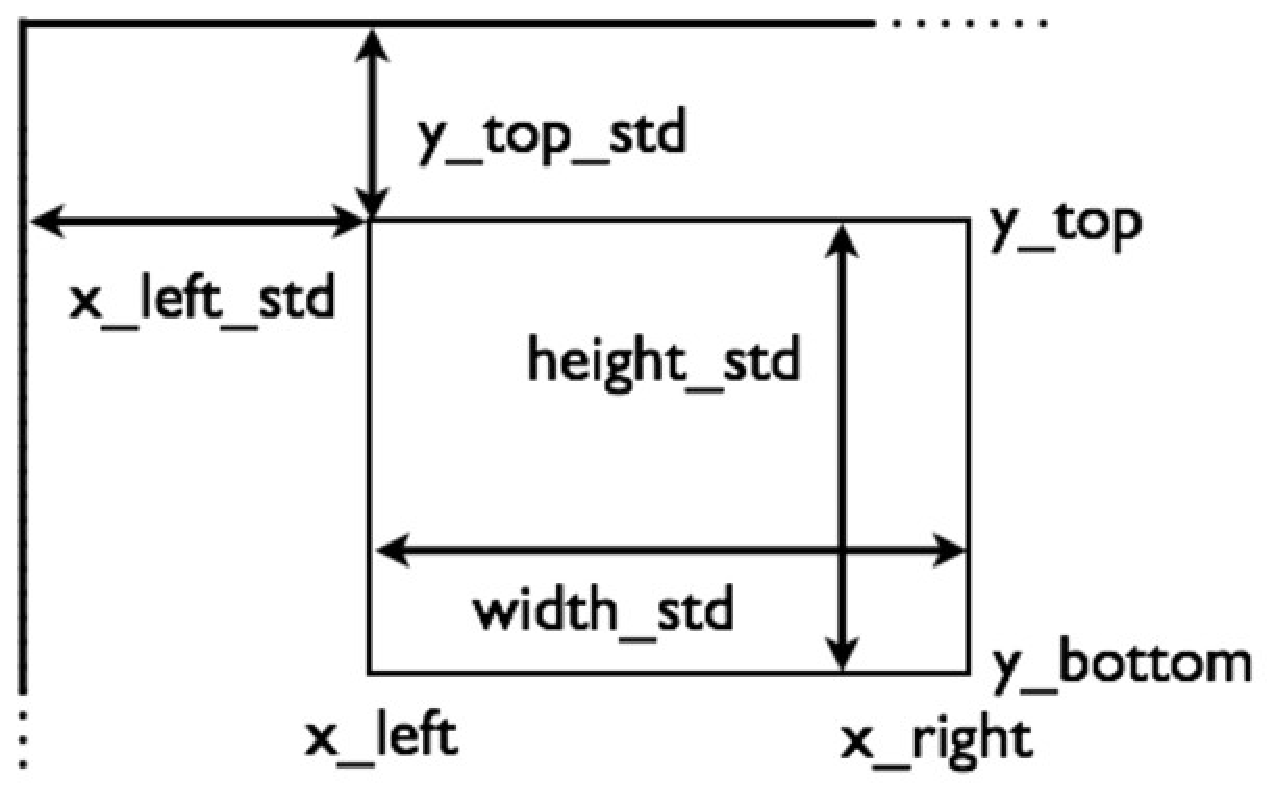
\includegraphics[width=100mm]{./Figures/eps/Canvas_g_def_scale_2D.eps}
\end{figure}
%%%%%%%%%%%%%%%%%%%%%%%%%%%%%%%%%%%%%%%%%%%%%%%%%%%%%%




%%%%%%%%%%%%%%%%%%%%%g_def_scale_3D%%%%%%%%%%%%%%%%%%%%%%%%%%%%%%
\clearpage
\subsubsection{\texttt{g\_def\_scale\_3D}}

\begin{itembox}[l]{\texttt{g\_def\_scale\_3D}関数}
%%%%%%%%%%%%%%%%%%%ここにプロトタイプ宣言を書く%%%%%%%%%%%%%%%%%%%
\begin{verbatim}
void g_def_scale_3D(
        int id,
        double x_left, double x_right,
        double y_bottom, double y_top,
        double z_near, double z_far,
        double x_left_std, double y_top_std,
        double width_std, double height_std,
        double direction_x, double direction_y, double direction_z
        double r);
\end{verbatim}
%%%%%%%%%%%%%%%%%%%ここに引数の説明を書く%%%%%%%%%%%%%%%%%%%%%%%
\verb|id| ; スケール番号\\
\verb|x_left,x_right,y_bottom,y_top,z_near,z_far| ; 描画したいx,y,z方向の範囲\\
\verb|x_left_std| ; 長方形の左辺の標準x座標\\
\verb|y_top_std| ; 長方形の上辺の標準y座標\\
\verb|width_std| ; 長方形の標準面上での幅\\
\verb|height_std| ; 長方形の標準面上での高さ\\
\verb|direction| ; 描画範囲で指定した直方体の重心に対する視点方向(図参照)\\
\verb|r| ; 視点距離 
\end{itembox}

%%%%%%%%%%%%%%%%%%%ここに関数の説明を書く%%%%%%%%%%%%%%%%%%%%%%%
\begin{itembox}[l]{\texttt{g\_def\_scale\_3D}関数の説明}
標準面上に3次元描画用の仮想座標系を定義する.座標軸は右手系で,y軸正方向が画面上になるように設定されている.
\end{itembox}

%%%%%%%%%%%%%%%%%%%ここに関数の説明に使う絵を載せる.%%%%%%%%%%%%%%%%
\begin{figure}[htb]
\centering
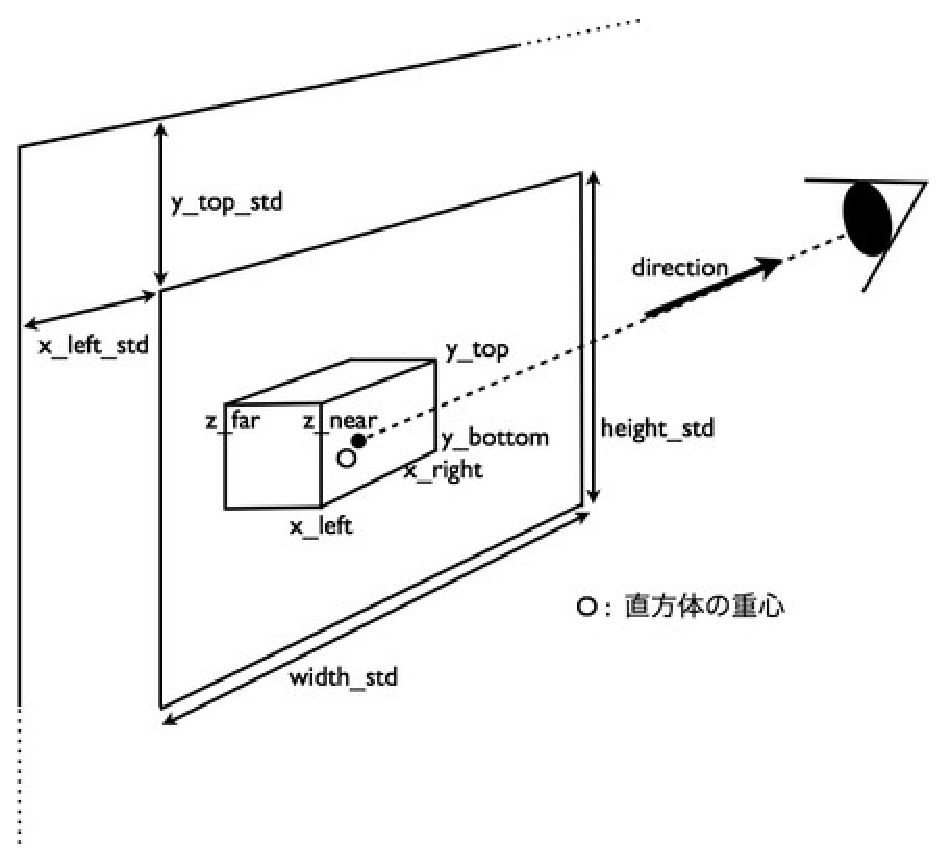
\includegraphics[width=100mm]{./Figures/eps/Canvas_g_def_scale_3D.eps}
\end{figure}
%%%%%%%%%%%%%%%%%%%%%%%%%%%%%%%%%%%%%%%%%%%%%%%%%%%%%%




%%%%%%%%%%%%%%%%%%%%%g_def_scale_3D_core%%%%%%%%%%%%%%%%%%%%%%%%%%%%%%
\clearpage
\subsubsection{\texttt{g\_def\_scale\_3D\_core}}

\begin{itembox}[l]{\texttt{g\_def\_scale\_3D\_core}関数}
%%%%%%%%%%%%%%%%%%%ここにプロトタイプ宣言を書く%%%%%%%%%%%%%%%%%%%
\begin{verbatim}
void g_def_scale_3D_core(
        int id,
        double x_left, double x_right,
        double y_bottom, double y_top,
        double z_near, double z_far,
        double x_left_std, double y_top_std,
        double width_std, double height_std,
        double direction_x, double direction_y, double direction_z,
        double r, double up_x, double up_y, double up_z);
\end{verbatim}
%%%%%%%%%%%%%%%%%%%ここに引数の説明を書く%%%%%%%%%%%%%%%%%%%%%%%
\verb|id| ; スケール番号\\
\verb|x_left,x_right,y_bottom,y_top,z_near,z_far| ; 描画したいx,y,z方向の範囲\\
\verb|x_left_std| ; 長方形の左辺の標準x座標\\
\verb|y_top_std| ; 長方形の上辺の標準y座標\\
\verb|width_std| ; 長方形の標準面上での幅\\
\verb|height_std| ; 長方形の標準面上での高さ\\
\verb|direction| ; 描画範囲で指定した直方体の重心に対する視点方向(図参照)\\
\verb|r| ; 視点距離 \\
\verb|up| ; 画面上方向の指定 
\end{itembox}

%%%%%%%%%%%%%%%%%%%ここに関数の説明を書く%%%%%%%%%%%%%%%%%%%%%%%
\begin{itembox}[l]{\texttt{g\_def\_scale\_3D\_core}関数の説明}
標準面上に3次元描画用の仮想座標系を定義する.画面上方向が設定可能になっている.
\end{itembox}




%%%%%%%%%%%%%%%%%%%%%g_sel_scale_2D,g_sel_scale_3D%%%%%%%%%%%%%%%%%%%%%%%%%%%%%%
\clearpage
\subsubsection{\texttt{g\_sel\_scale\_2D, g\_sel\_scale\_3D}}

\begin{itembox}[l]{\texttt{g\_sel\_scale\_2D, g\_sel\_scale\_3D}関数}
%%%%%%%%%%%%%%%%%%%ここにプロトタイプ宣言を書く%%%%%%%%%%%%%%%%%%%
\begin{verbatim}
void g_sel_scale_2D(
        int id);
void g_sel_scale_3D(
        int id);
\end{verbatim}
%%%%%%%%%%%%%%%%%%%ここに引数の説明を書く%%%%%%%%%%%%%%%%%%%%%%%
\verb|id| ; スケール番号
\end{itembox}

%%%%%%%%%%%%%%%%%%%ここに関数の説明を書く%%%%%%%%%%%%%%%%%%%%%%%
\begin{itembox}[l]{\texttt{g\_sel\_scale\_2D, g\_sel\_scale\_3D}関数の説明}
仮想座標系を選択する.
\end{itembox}




%%%%%%%%%%%%%%%%%%%%%g_sel_scale_2D_boundary,g_sel_scale_3D_boundary%%%%%%%%%%%%%%%%%%%%%%%%%%%%%%
\subsubsection{\texttt{g\_sel\_scale\_2D\_boundary, g\_sel\_scale\_3D\_boundary}}

\begin{itembox}[l]{\texttt{g\_sel\_scale\_2D\_boundary, g\_sel\_scale\_3D\_boundary}関数}
%%%%%%%%%%%%%%%%%%%ここにプロトタイプ宣言を書く%%%%%%%%%%%%%%%%%%%
\begin{verbatim}
void g_sel_scale_2D_boundary(
        int id);
void g_sel_scale_3D_boundary(
        int id);
\end{verbatim}
%%%%%%%%%%%%%%%%%%%ここに引数の説明を書く%%%%%%%%%%%%%%%%%%%%%%%
\verb|id| ; スケール番号
\end{itembox}

%%%%%%%%%%%%%%%%%%%ここに関数の説明を書く%%%%%%%%%%%%%%%%%%%%%%%
\begin{itembox}[l]{\texttt{g\_sel\_scale\_2D\_boundary, g\_sel\_scale\_3D\_boundary}関数の説明}
仮想座標系を選択し,選択された仮想座標系の枠を表示する.
\end{itembox}




\clearpage
\subsection{属性コントロール関数}

%%%%%%%%%%%%%%%%%%%%%g_marker_color%%%%%%%%%%%%%%%%%%%%%%%%%%%%%%
\subsubsection{\texttt{g\_marker\_color}}

\begin{itembox}[l]{\texttt{g\_marker\_color}関数}
%%%%%%%%%%%%%%%%%%%ここにプロトタイプ宣言を書く%%%%%%%%%%%%%%%%%%%
\begin{verbatim}
void g_marker_color(
        float r, float g, float b, float a);
\end{verbatim}
%%%%%%%%%%%%%%%%%%%ここに引数の説明を書く%%%%%%%%%%%%%%%%%%%%%%%
\verb|r,g,b,a| ; 光の三原色+不透明度($0\leq \verb|r,g,b,a| \leq 1$)
\end{itembox}

%%%%%%%%%%%%%%%%%%%ここに関数の説明を書く%%%%%%%%%%%%%%%%%%%%%%%
\begin{itembox}[l]{\texttt{g\_marker\_color}関数の説明}
マーカーの色を変更する.
\end{itembox}

%%%%%%%%%%%%%%%%%%%%%g_marker_size%%%%%%%%%%%%%%%%%%%%%%%%%%%%%%
\subsubsection{\texttt{g\_marker\_size}}

\begin{itembox}[l]{\texttt{g\_marker\_size}関数}
%%%%%%%%%%%%%%%%%%%ここにプロトタイプ宣言を書く%%%%%%%%%%%%%%%%%%%
\begin{verbatim}
void g_marker_size(
        float size);
\end{verbatim}
%%%%%%%%%%%%%%%%%%%ここに引数の説明を書く%%%%%%%%%%%%%%%%%%%%%%%
\verb|size| ; マーカーの大きさ(ピクセル単位)
\end{itembox}

%%%%%%%%%%%%%%%%%%%ここに関数の説明を書く%%%%%%%%%%%%%%%%%%%%%%%
\begin{itembox}[l]{\texttt{g\_marker\_size}関数の説明}
マーカーの大きさを変更する.ピクセル単位の直径を指定する.
\end{itembox}

%%%%%%%%%%%%%%%%%%%%%g_marker_radius%%%%%%%%%%%%%%%%%%%%%%%%%%%%%%
\subsubsection{\texttt{g\_marker\_radius}}

\begin{itembox}[l]{\texttt{g\_marker\_radius}関数}
%%%%%%%%%%%%%%%%%%%ここにプロトタイプ宣言を書く%%%%%%%%%%%%%%%%%%%
\begin{verbatim}
void g_marker_radius(
        float size);
\end{verbatim}
%%%%%%%%%%%%%%%%%%%ここに引数の説明を書く%%%%%%%%%%%%%%%%%%%%%%%
\verb|size| ; マーカーの大きさ(仮想座標系での半径)
\end{itembox}

%%%%%%%%%%%%%%%%%%%ここに関数の説明を書く%%%%%%%%%%%%%%%%%%%%%%%
\begin{itembox}[l]{\texttt{g\_marker\_radius}関数の説明}
	マーカーの大きさを変更する.仮想座標系での半径を指定する.
\end{itembox}

%%%%%%%%%%%%%%%%%%%%%g_marker_type%%%%%%%%%%%%%%%%%%%%%%%%%%%%%%
\clearpage

\subsubsection{\texttt{g\_marker\_type}}

\begin{itembox}[l]{\texttt{g\_marker\_type}関数}
%%%%%%%%%%%%%%%%%%%ここにプロトタイプ宣言を書く%%%%%%%%%%%%%%%%%%%
\begin{verbatim}
void g_marker_type(
        unsigned int type);
\end{verbatim}
%%%%%%%%%%%%%%%%%%%ここに引数の説明を書く%%%%%%%%%%%%%%%%%%%%%%%
\verb|type| ; マーカーの種類
\end{itembox}

%%%%%%%%%%%%%%%%%%%ここに関数の説明を書く%%%%%%%%%%%%%%%%%%%%%%%
\begin{itembox}[l]{\texttt{g\_marker\_type}関数の説明}
マーカーの種類を変更する.使用できるマーカーの種類は以下の通り.
\begin{center}
\begin{tabular}{|c|c|c|}
	\hline 
	定数名 & 値 & 形状 \\ 
	\hline 
	\verb|G_MARKER_SQUARE| & 0 & 正方形 \\ 
	\hline 
	\verb|G_MARKER_CIRCLE| & 1 & 円 \\ 
	\hline 
	\verb|G_MARKER_SPHERE| & 2 & 球 \\ 
	\hline 
\end{tabular}
\end{center}
\end{itembox}

\begin{itembox}[l]{マーカーに関するパフォーマンス上の注意}
マーカータイプの変更はシェーダーの切り替えを伴うため,できるだけ同じ種類のマーカーをまとめて描画するようにすること.

また,マーカーサイズの変更は問題ないが,マーカーサイズの座標系(\verb|g_marker_size|または\verb|g_marker_radius|)の変更もシェーダーの切り替えを伴うため,できるだけ同じ座標系のマーカーサイズをまとめて使用すること.
\end{itembox}

%%%%%%%%%%%%%%%%%%%%%g_def_marker%%%%%%%%%%%%%%%%%%%%%%%%%%%%%%
\clearpage
\subsubsection{\texttt{g\_def\_marker}}

\begin{itembox}[l]{\texttt{g\_def\_marker}関数}
%%%%%%%%%%%%%%%%%%%ここにプロトタイプ宣言を書く%%%%%%%%%%%%%%%%%%%
\begin{verbatim}
void g_def_marker(
        int id,
        float r, float b, float g, float a,
        int type, float size);
\end{verbatim}
%%%%%%%%%%%%%%%%%%%ここに引数の説明を書く%%%%%%%%%%%%%%%%%%%%%%%
\verb|id| ; マーカーの属性番号\\
\verb|r,g,b,a| ; 光の三原色+不透明度($0\leq \verb|r,g,b,a| \leq 1$)\\
\verb|type| ; マーカーの種類(\verb|g_marker_type|の説明を参照)\\
\verb|size| ; マーカーの大きさ
\end{itembox}

%%%%%%%%%%%%%%%%%%%ここに関数の説明を書く%%%%%%%%%%%%%%%%%%%%%%%
\begin{itembox}[l]{\texttt{g\_def\_marker}関数の説明}
マーカーの属性セットを定義する.
\end{itembox}

\subsubsection{\texttt{g\_sel\_marker}}

\begin{itembox}[l]{\texttt{g\_sel\_marker}関数}
%%%%%%%%%%%%%%%%%%%ここにプロトタイプ宣言を書く%%%%%%%%%%%%%%%%%%%
\begin{verbatim}
void g_sel_marker(
        int id);
\end{verbatim}
%%%%%%%%%%%%%%%%%%%ここに引数の説明を書く%%%%%%%%%%%%%%%%%%%%%%%
\verb|id| ; マーカーの属性番号
\end{itembox}

%%%%%%%%%%%%%%%%%%%ここに関数の説明を書く%%%%%%%%%%%%%%%%%%%%%%%
\begin{itembox}[l]{\texttt{g\_sel\_marker}関数の説明}
マーカーの属性セットを選択する.
\end{itembox}

%%%%%%%%%%%%%%%%%%%ここに関数の説明に使う絵を載せる.%%%%%%%%%%%%%%%%
\begin{figure}[htb]
\centering
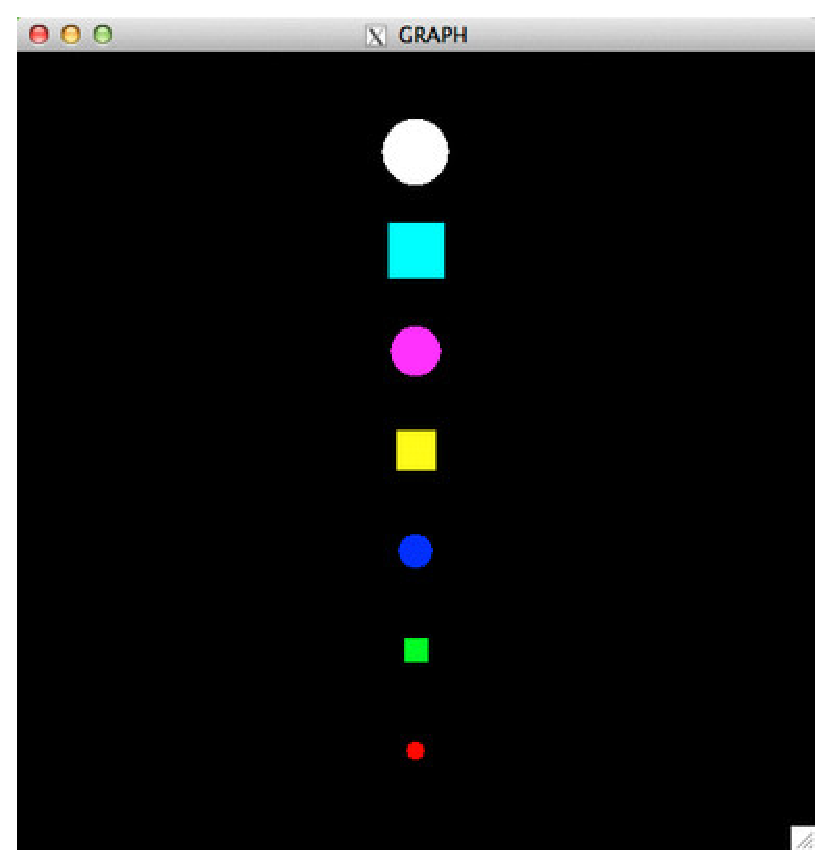
\includegraphics[width=100mm]{./Figures/eps/Canvas_g_marker.eps}
\end{figure}
%%%%%%%%%%%%%%%%%%%%%%%%%%%%%%%%%%%%%%%%%%%%%%%%%%%%%%


%%%%%%%%%%%%%%%%%%%%%g_line_color%%%%%%%%%%%%%%%%%%%%%%%%%%%%%%
\clearpage
\subsubsection{\texttt{g\_line\_color}}

\begin{itembox}[l]{\texttt{g\_line\_color}関数}
%%%%%%%%%%%%%%%%%%%ここにプロトタイプ宣言を書く%%%%%%%%%%%%%%%%%%%
\begin{verbatim}
void g_line_color(
        float r,float g,float b,float a);
\end{verbatim}
%%%%%%%%%%%%%%%%%%%ここに引数の説明を書く%%%%%%%%%%%%%%%%%%%%%%%
\verb|r,g,b,a| ; 光の三原色+不透明度($0\leq \verb|r,g,b,a| \leq 1$)
\end{itembox}

%%%%%%%%%%%%%%%%%%%ここに関数の説明を書く%%%%%%%%%%%%%%%%%%%%%%%
\begin{itembox}[l]{\texttt{g\_line\_color}関数の説明}
線の色を変更する.
\end{itembox}

%%%%%%%%%%%%%%%%%%%%%g_line_width%%%%%%%%%%%%%%%%%%%%%%%%%%%%%%
\subsubsection{\texttt{g\_line\_width}}

\begin{itembox}[l]{\texttt{g\_line\_width}関数}
%%%%%%%%%%%%%%%%%%%ここにプロトタイプ宣言を書く%%%%%%%%%%%%%%%%%%%
\begin{verbatim}
void g_line_width(
        float size);
\end{verbatim}
%%%%%%%%%%%%%%%%%%%ここに引数の説明を書く%%%%%%%%%%%%%%%%%%%%%%%
\verb|size| ; 線の太さ
\end{itembox}

%%%%%%%%%%%%%%%%%%%ここに関数の説明を書く%%%%%%%%%%%%%%%%%%%%%%%
\begin{itembox}[l]{\texttt{g\_line\_width}関数の説明}
線の太さを変更する.(0は1と同じ太さになることに注意)
\end{itembox}

%%%%%%%%%%%%%%%%%%%%%g_line_type%%%%%%%%%%%%%%%%%%%%%%%%%%%%%%
\subsubsection{\texttt{g\_line\_type}}

\begin{itembox}[l]{\texttt{g\_line\_type}関数}
%%%%%%%%%%%%%%%%%%%ここにプロトタイプ宣言を書く%%%%%%%%%%%%%%%%%%%
\begin{verbatim}
void g_line_type(
        int type);
\end{verbatim}
%%%%%%%%%%%%%%%%%%%ここに引数の説明を書く%%%%%%%%%%%%%%%%%%%%%%%
\verb|type| ; 線の種類(0〜8)
\end{itembox}

%%%%%%%%%%%%%%%%%%%ここに関数の説明を書く%%%%%%%%%%%%%%%%%%%%%%%
\begin{itembox}[l]{\texttt{g\_line\_type}関数の説明}
線の種類を変更する.
\end{itembox}

%%%%%%%%%%%%%%%%%%%ここに関数の説明に使う絵を載せる.%%%%%%%%%%%%%%%%
\begin{figure}[htb]
\end{figure}
%%%%%%%%%%%%%%%%%%%%%%%%%%%%%%%%%%%%%%%%%%%%%%%%%%%%%%



%%%%%%%%%%%%%%%%%%%%%g_def_line%%%%%%%%%%%%%%%%%%%%%%%%%%%%%%
\clearpage
\subsubsection{\texttt{g\_def\_line}}

\begin{itembox}[l]{\texttt{g\_def\_line}関数}
%%%%%%%%%%%%%%%%%%%ここにプロトタイプ宣言を書く%%%%%%%%%%%%%%%%%%%
\begin{verbatim}
void g_def_line(
        int id,	
        float r, float b, float g, float a,
        float width, int type);
\end{verbatim}
%%%%%%%%%%%%%%%%%%%ここに引数の説明を書く%%%%%%%%%%%%%%%%%%%%%%%
\verb|id| ; 線の属性番号\\
\verb|r,g,b,a| ; 光の三原色+不透明度($0\leq \verb|r,g,b,a| \leq 1$)\\
\verb|width| ; 線の太さ\\
\verb|type| ; 線の種類(0〜8)
\end{itembox}

%%%%%%%%%%%%%%%%%%%ここに関数の説明を書く%%%%%%%%%%%%%%%%%%%%%%%
\begin{itembox}[l]{\texttt{g\_def\_line}関数の説明}
線の属性セットを定義する.
\end{itembox}

%%%%%%%%%%%%%%%%%%%ここに関数の説明に使う絵を載せる.%%%%%%%%%%%%%%%%
\begin{figure}[htb]
\end{figure}
%%%%%%%%%%%%%%%%%%%%%%%%%%%%%%%%%%%%%%%%%%%%%%%%%%%%%%



%%%%%%%%%%%%%%%%%%%%%g_sel_line%%%%%%%%%%%%%%%%%%%%%%%%%%%%%%
\clearpage
\subsubsection{\texttt{g\_sel\_line}}

\begin{itembox}[l]{\texttt{g\_sel\_line}関数}
%%%%%%%%%%%%%%%%%%%ここにプロトタイプ宣言を書く%%%%%%%%%%%%%%%%%%%
\begin{verbatim}
void g_sel_line(
        int id);
\end{verbatim}
%%%%%%%%%%%%%%%%%%%ここに引数の説明を書く%%%%%%%%%%%%%%%%%%%%%%%
\verb|id| ; 線の属性番号
\end{itembox}

%%%%%%%%%%%%%%%%%%%ここに関数の説明を書く%%%%%%%%%%%%%%%%%%%%%%%
\begin{itembox}[l]{\texttt{g\_sel\_line}関数の説明}
線の属性セットを選択する.
\end{itembox}

%%%%%%%%%%%%%%%%%%%ここに関数の説明に使う絵を載せる.%%%%%%%%%%%%%%%%
\begin{figure}[htb]
\centering
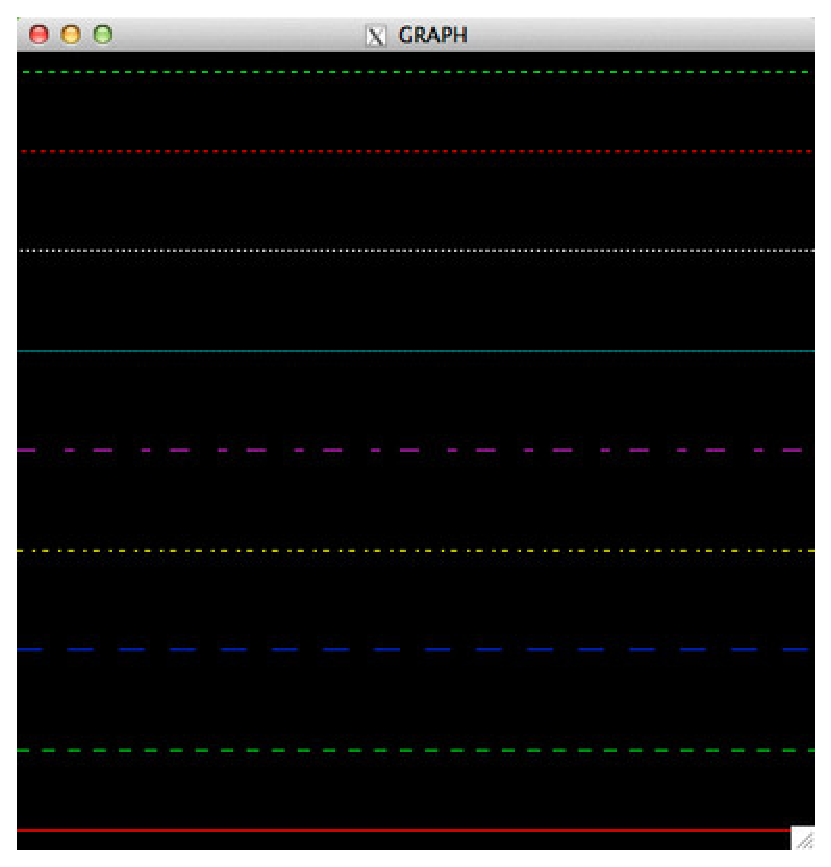
\includegraphics[width=100mm]{./Figures/eps/Canvas_g_line.eps}
\end{figure}
%%%%%%%%%%%%%%%%%%%%%%%%%%%%%%%%%%%%%%%%%%%%%%%%%%%%%%





%%%%%%%%%%%%%%%%%%%%%g_area_color_2D,g_area_color_2D%%%%%%%%%%%%%%%%%%%%%%%%%%%%%%
\clearpage
\subsubsection{\texttt{g\_area\_color\_2D,g\_area\_color\_3D}}

\begin{itembox}[l]{\texttt{g\_area\_color\_2D,g\_area\_color\_3D}関数}
%%%%%%%%%%%%%%%%%%%ここにプロトタイプ宣言を書く%%%%%%%%%%%%%%%%%%%
\begin{verbatim}
void g_area_color_2D(
        float r, float g, float b, float a);
void g_area_color_3D(
        float r, float g, float b, float a);
\end{verbatim}
%%%%%%%%%%%%%%%%%%%ここに引数の説明を書く%%%%%%%%%%%%%%%%%%%%%%%
\verb|r,g,b,a| ; 光の三原色+不透明度($0\leq \verb|r,g,b,a| \leq 1$)
\end{itembox}

%%%%%%%%%%%%%%%%%%%ここに関数の説明を書く%%%%%%%%%%%%%%%%%%%%%%%
\begin{itembox}[l]{\texttt{g\_area\_color\_2D,g\_area\_color\_3D}関数の説明}
面を塗りつぶす色を変更する.
\end{itembox}

%%%%%%%%%%%%%%%%%%%ここに関数の説明に使う絵を載せる.%%%%%%%%%%%%%%%%
\begin{figure}[htb]
\centering
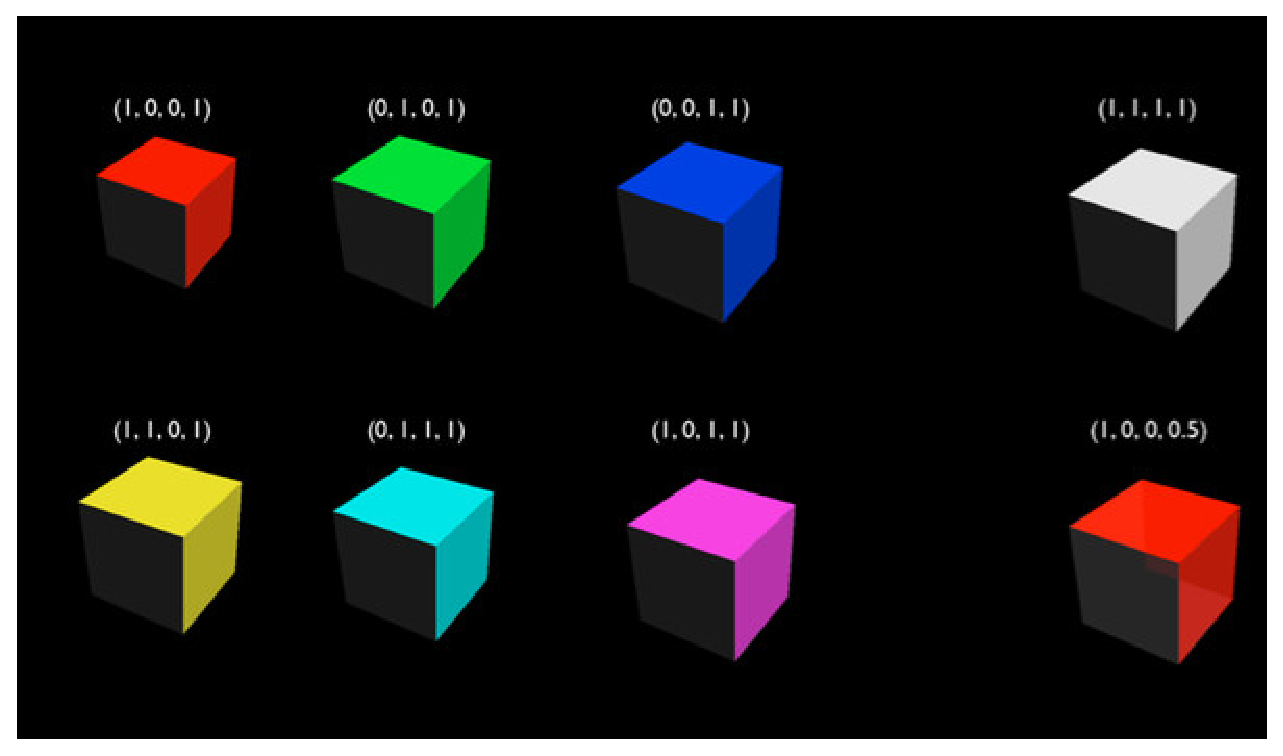
\includegraphics[width=100mm]{./Figures/eps/Canvas_g_area_color.eps}
\end{figure}
%%%%%%%%%%%%%%%%%%%%%%%%%%%%%%%%%%%%%%%%%%%%%%%%%%%%%%

%%%%%%%%%%%%%%%%%%%%%g_def_area_2D,g_def_area_3D%%%%%%%%%%%%%%%%%%%%%%%%%%%%%%
\clearpage
\subsubsection{\texttt{g\_def\_area\_2D,g\_def\_area\_3D}}

\begin{itembox}[l]{\texttt{g\_def\_area\_2D,g\_def\_area\_3D}関数}
%%%%%%%%%%%%%%%%%%%ここにプロトタイプ宣言を書く%%%%%%%%%%%%%%%%%%%
\begin{verbatim}
void g_def_area_2D(
        int id,	
        float r, float b, float g, float a);
void g_def_area_3D(
        int id,	
        float r, float b, float g, float a);
\end{verbatim}
%%%%%%%%%%%%%%%%%%%ここに引数の説明を書く%%%%%%%%%%%%%%%%%%%%%%%
\verb|id| ; 塗りつぶしの属性番号\\
\verb|r,g,b,a| ; 光の三原色+不透明度($0\leq \verb|r,g,b,a| \leq 1$)
\end{itembox}

%%%%%%%%%%%%%%%%%%%ここに関数の説明を書く%%%%%%%%%%%%%%%%%%%%%%%
\begin{itembox}[l]{\texttt{g\_def\_area\_2D,g\_def\_area\_3D}関数の説明}
塗りつぶしの属性セットを定義する.
\end{itembox}

%%%%%%%%%%%%%%%%%%%%%g_sel_area_2D,g_sel_area_3D%%%%%%%%%%%%%%%%%%%%%%%%%%%%%%
\subsubsection{\texttt{g\_sel\_area\_2D,g\_sel\_area\_3D}}

\begin{itembox}[l]{\texttt{g\_sel\_area\_2D,g\_sel\_area\_3D}関数}
%%%%%%%%%%%%%%%%%%%ここにプロトタイプ宣言を書く%%%%%%%%%%%%%%%%%%%
\begin{verbatim}
void g_sel_area_2D(
        int id);
void g_sel_area_3D(
        int id);
\end{verbatim}
%%%%%%%%%%%%%%%%%%%ここに引数の説明を書く%%%%%%%%%%%%%%%%%%%%%%%
\verb|id| ; 塗りつぶしの属性番号
\end{itembox}

%%%%%%%%%%%%%%%%%%%ここに関数の説明を書く%%%%%%%%%%%%%%%%%%%%%%%
\begin{itembox}[l]{\texttt{g\_sel\_area\_2D,g\_sel\_area\_3D}関数の説明}
塗りつぶしの属性セットを選択する.
\end{itembox}


%%%%%%%%%%%%%%%%%%%%%g_text_color%%%%%%%%%%%%%%%%%%%%%%%%%%%%%%
\clearpage
\subsubsection{\texttt{g\_text\_color}}

\begin{itembox}[l]{\texttt{g\_text\_color}関数}
%%%%%%%%%%%%%%%%%%%ここにプロトタイプ宣言を書く%%%%%%%%%%%%%%%%%%%
\begin{verbatim}
void g_text_color(
        float r, float g, float b, float a);
\end{verbatim}
%%%%%%%%%%%%%%%%%%%ここに引数の説明を書く%%%%%%%%%%%%%%%%%%%%%%%
\verb|r,g,b,a| ; 光の三原色+不透明度($0\leq \verb|r,g,b,a| \leq 1$)\\
\end{itembox}

%%%%%%%%%%%%%%%%%%%ここに関数の説明を書く%%%%%%%%%%%%%%%%%%%%%%%
\begin{itembox}[l]{\texttt{g\_text\_color}関数の説明}
テキストの色を変更する.
\end{itembox}

%%%%%%%%%%%%%%%%%%%%%g_text_font_core%%%%%%%%%%%%%%%%%%%%%%%%%%%%%%
\subsubsection{\texttt{g\_text\_font\_core}}

\begin{itembox}[l]{\texttt{g\_text\_font\_core}関数}
%%%%%%%%%%%%%%%%%%%ここにプロトタイプ宣言を書く%%%%%%%%%%%%%%%%%%%
\begin{verbatim}
void g_text_font_core(
        const char *font_file);
\end{verbatim}
%%%%%%%%%%%%%%%%%%%ここに引数の説明を書く%%%%%%%%%%%%%%%%%%%%%%%
\verb|const char *font_file| ; テキストのフォントを相対パス名で指定する.テキストのフォントはttf(True Type Font), otf(Open Type Font)などの主要な形式を指定できる.\\
\end{itembox}

%%%%%%%%%%%%%%%%%%%ここに関数の説明を書く%%%%%%%%%%%%%%%%%%%%%%%
\begin{itembox}[l]{\texttt{g\_text\_font\_core}関数の説明}
テキストのフォントを変更する.
\end{itembox}

%%%%%%%%%%%%%%%%%%%%%g_text_size%%%%%%%%%%%%%%%%%%%%%%%%%%%%%%
\subsubsection{\texttt{g\_text\_size}}

\begin{itembox}[l]{\texttt{g\_text\_size}関数}
	%%%%%%%%%%%%%%%%%%%ここにプロトタイプ宣言を書く%%%%%%%%%%%%%%%%%%%
	\begin{verbatim}
	void g_text_size(
        float size);
	\end{verbatim}
	%%%%%%%%%%%%%%%%%%%ここに引数の説明を書く%%%%%%%%%%%%%%%%%%%%%%%
	\verb|size| ; テキストのサイズを指定する.
\end{itembox}

%%%%%%%%%%%%%%%%%%%ここに関数の説明を書く%%%%%%%%%%%%%%%%%%%%%%%
\begin{itembox}[l]{\texttt{g\_text\_font\_core}関数の説明}
	テキストのサイズを変更する.
\end{itembox}


%%%%%%%%%%%%%%%%%%%%%g_def_text%%%%%%%%%%%%%%%%%%%%%%%%%%%%%%
\clearpage
\subsubsection{\texttt{g\_def\_text, g\_def\_text\_core, g\_sel\_text}}

\begin{itembox}[l]{\texttt{g\_def\_text}関数}
%%%%%%%%%%%%%%%%%%%ここにプロトタイプ宣言を書く%%%%%%%%%%%%%%%%%%%
\begin{verbatim}
void g_def_text(
        int id,
        float r, float g, float b, float a,
        unsigned int font_size);
\end{verbatim}
%%%%%%%%%%%%%%%%%%%ここに引数の説明を書く%%%%%%%%%%%%%%%%%%%%%%%
\verb|id| ; テキストの属性番号\\
\verb|r,g,b,a| ; 光の三原色+不透明度($0\leq \verb|r,g,b,a| \leq 1$)\\
%\verb|font| ; 使用されません\\
\verb|font_size| ; テキストのサイズ(自然数)
\end{itembox}

%%%%%%%%%%%%%%%%%%%ここに関数の説明を書く%%%%%%%%%%%%%%%%%%%%%%%
\begin{itembox}[l]{\texttt{g\_def\_text}関数の説明}
テキストの属性セットを定義する.
%\verb|font|引数は無視される.
\end{itembox}

%%%%%%%%%%%%%%%%%%%%%g_def_text_core%%%%%%%%%%%%%%%%%%%%%%%%%%%%%%


\begin{itembox}[l]{\texttt{g\_def\_text\_core}関数}
%%%%%%%%%%%%%%%%%%%ここにプロトタイプ宣言を書く%%%%%%%%%%%%%%%%%%%
\begin{verbatim}
void g_def_text_core(
        int id,
        float r, float g, float b, float a,
        const char *font_type, unsigned int font_size);
\end{verbatim}
%%%%%%%%%%%%%%%%%%%ここに引数の説明を書く%%%%%%%%%%%%%%%%%%%%%%%
\verb|id| ; テキストの属性番号\\
\verb|r,g,b,a| ; 光の三原色+不透明度($0\leq \verb|r,g,b,a| \leq 1$)\\
\verb|font_type| ; フォントファイル名,または\verb|NULL|\\
\verb|font_size| ; テキストのサイズ(自然数)
\end{itembox}

%%%%%%%%%%%%%%%%%%%ここに関数の説明を書く%%%%%%%%%%%%%%%%%%%%%%%
\begin{itembox}[l]{\texttt{g\_def\_text}関数の説明}
	テキストの属性セットを定義する.\verb|font_type==NULL|のとき,色とサイズのみ使用される.
\end{itembox}

\begin{itembox}[l]{\texttt{g\_sel\_text}関数}
%%%%%%%%%%%%%%%%%%%ここにプロトタイプ宣言を書く%%%%%%%%%%%%%%%%%%%
\begin{verbatim}
void g_sel_text(
        int id);
\end{verbatim}
%%%%%%%%%%%%%%%%%%%ここに引数の説明を書く%%%%%%%%%%%%%%%%%%%%%%%
\verb|id| ; 線の属性番号
\end{itembox}

%%%%%%%%%%%%%%%%%%%ここに関数の説明を書く%%%%%%%%%%%%%%%%%%%%%%%
\begin{itembox}[l]{\texttt{g\_sel\_text}関数の説明}
テキストの属性セットを選択する.
\end{itembox}




\clearpage
\subsection{描画関数}
%%%%%%%%%%%%%%%%%%%%%g_marker_2D,g_marker_3D%%%%%%%%%%%%%%%%%%%%%%%%%%%%%%
\subsubsection{\texttt{g\_marker\_2D, g\_marker\_3D}}

\begin{itembox}[l]{\texttt{g\_marker\_2D, g\_marker\_3D}関数}
%%%%%%%%%%%%%%%%%%%ここにプロトタイプ宣言を書く%%%%%%%%%%%%%%%%%%%
\begin{verbatim}
void g_marker_2D(
        double x, double y);
void g_marker_3D(
        double x, double y, double z);	
\end{verbatim}
%%%%%%%%%%%%%%%%%%%ここに引数の説明を書く%%%%%%%%%%%%%%%%%%%%%%%
\verb|x,y,z| ; マーカーの中心座標
\end{itembox}

%%%%%%%%%%%%%%%%%%%ここに関数の説明を書く%%%%%%%%%%%%%%%%%%%%%%%
\begin{itembox}[l]{\texttt{g\_marker\_2D, g\_marker\_3D}関数の説明}
マーカーを描画する.
\end{itembox}

%%%%%%%%%%%%%%%%%%%ここに関数の説明に使う絵を載せる.%%%%%%%%%%%%%%%%
\begin{figure}[htb]
\end{figure}
%%%%%%%%%%%%%%%%%%%%%%%%%%%%%%%%%%%%%%%%%%%%%%%%%%%%%%




%%%%%%%%%%%%%%%%%%%%%g_text_standard%%%%%%%%%%%%%%%%%%%%%%%%%%%%%%
\clearpage
\subsubsection{\texttt{g\_text\_standard}}

\begin{itembox}[l]{\texttt{g\_text\_standard}関数}
%%%%%%%%%%%%%%%%%%%ここにプロトタイプ宣言を書く%%%%%%%%%%%%%%%%%%%
\begin{verbatim}
void g_text_standard(
        double x, double y,
        const char *str);
\end{verbatim}
%%%%%%%%%%%%%%%%%%%ここに引数の説明を書く%%%%%%%%%%%%%%%%%%%%%%%
\verb|x,y| ; テキスト左下の座標(標準座標系)\\
\verb|str| ; 文字列
\end{itembox}

%%%%%%%%%%%%%%%%%%%ここに関数の説明を書く%%%%%%%%%%%%%%%%%%%%%%%
\begin{itembox}[l]{\texttt{g\_text\_standard}関数の説明}
文字列を描画する.
(座標指定が標準座標系であることに注意.)
\end{itembox}


%%%%%%%%%%%%%%%%%%%%%g_text_virtual_2D,g_text_virtual_3D%%%%%%%%%%%%%%%%%%%%%%%%%%%%%%
\subsubsection{\texttt{g\_text\_virtual\_2D,g\_text\_virtual\_3D}}

\begin{itembox}[l]{\texttt{g\_text\_virtual\_2D,g\_text\_virtual\_3D}関数}
%%%%%%%%%%%%%%%%%%%ここにプロトタイプ宣言を書く%%%%%%%%%%%%%%%%%%%
\begin{verbatim}
void g_text_2D_virtual(
        double x, double y,
        const char *str);
void g_text_3D_virtual(
        double x, double y, double z,
        const char *str);      
\end{verbatim}
%%%%%%%%%%%%%%%%%%%ここに引数の説明を書く%%%%%%%%%%%%%%%%%%%%%%%
\verb|x,y,z| ; テキスト左下の座標(仮想座標系)\\
\verb|str| ; 文字列
\end{itembox}

%%%%%%%%%%%%%%%%%%%ここに関数の説明を書く%%%%%%%%%%%%%%%%%%%%%%%
\begin{itembox}[l]{\texttt{g\_text\_virtual\_2D,g\_text\_virtual\_3D}関数の説明}
文字列を描画する.
(座標指定が仮想座標系であることに注意.)
\end{itembox}

%%%%%%%%%%%%%%%%%%%ここに関数の説明に使う絵を載せる.%%%%%%%%%%%%%%%%
\begin{figure}[htb]
\end{figure}
%%%%%%%%%%%%%%%%%%%%%%%%%%%%%%%%%%%%%%%%%%%%%%%%%%%%%%




%%%%%%%%%%%%%%%%%%%%%g_move_2D,g_move_3D%%%%%%%%%%%%%%%%%%%%%%%%%%%%%%
\clearpage
\subsubsection{\texttt{g\_move\_2D,g\_move\_3D}}

\begin{itembox}[l]{\texttt{g\_move\_2D,g\_move\_3D}関数}
%%%%%%%%%%%%%%%%%%%ここにプロトタイプ宣言を書く%%%%%%%%%%%%%%%%%%%
\begin{verbatim}
void g_move_2D(
        double x, double y);
void g_move_3D(
        double x, double y, double z);     
\end{verbatim}
%%%%%%%%%%%%%%%%%%%ここに引数の説明を書く%%%%%%%%%%%%%%%%%%%%%%%
\verb|x,y,z| ; 線の始点の座標\\
\end{itembox}

%%%%%%%%%%%%%%%%%%%ここに関数の説明を書く%%%%%%%%%%%%%%%%%%%%%%%
\begin{itembox}[l]{\texttt{g\_move\_2D,g\_move\_3D}関数の説明}
線の始点を指定する.
\end{itembox}

%%%%%%%%%%%%%%%%%%%%%g_plot_2D,g_plot_3D%%%%%%%%%%%%%%%%%%%%%%%%%%%%%%
\subsubsection{\texttt{g\_plot\_2D,g\_plot\_3D}}

\begin{itembox}[l]{\texttt{g\_plot\_2D,g\_plot\_3D}関数}
%%%%%%%%%%%%%%%%%%%ここにプロトタイプ宣言を書く%%%%%%%%%%%%%%%%%%%
\begin{verbatim}
void g_plot_2D(
        double x, double y);
void g_plot_3D(
        double x, double y, double z);     
\end{verbatim}
%%%%%%%%%%%%%%%%%%%ここに引数の説明を書く%%%%%%%%%%%%%%%%%%%%%%%
\verb|x,y,z| ; 線の始点の座標\\
\end{itembox}

%%%%%%%%%%%%%%%%%%%ここに関数の説明を書く%%%%%%%%%%%%%%%%%%%%%%%
\begin{itembox}[l]{\texttt{g\_plot\_2D,g\_plot\_3D}関数の説明}
線の終点を指定する.
\end{itembox}

%%%%%%%%%%%%%%%%%%%ここに関数の説明に使う絵を載せる.%%%%%%%%%%%%%%%%
\begin{figure}[htb]
\centering
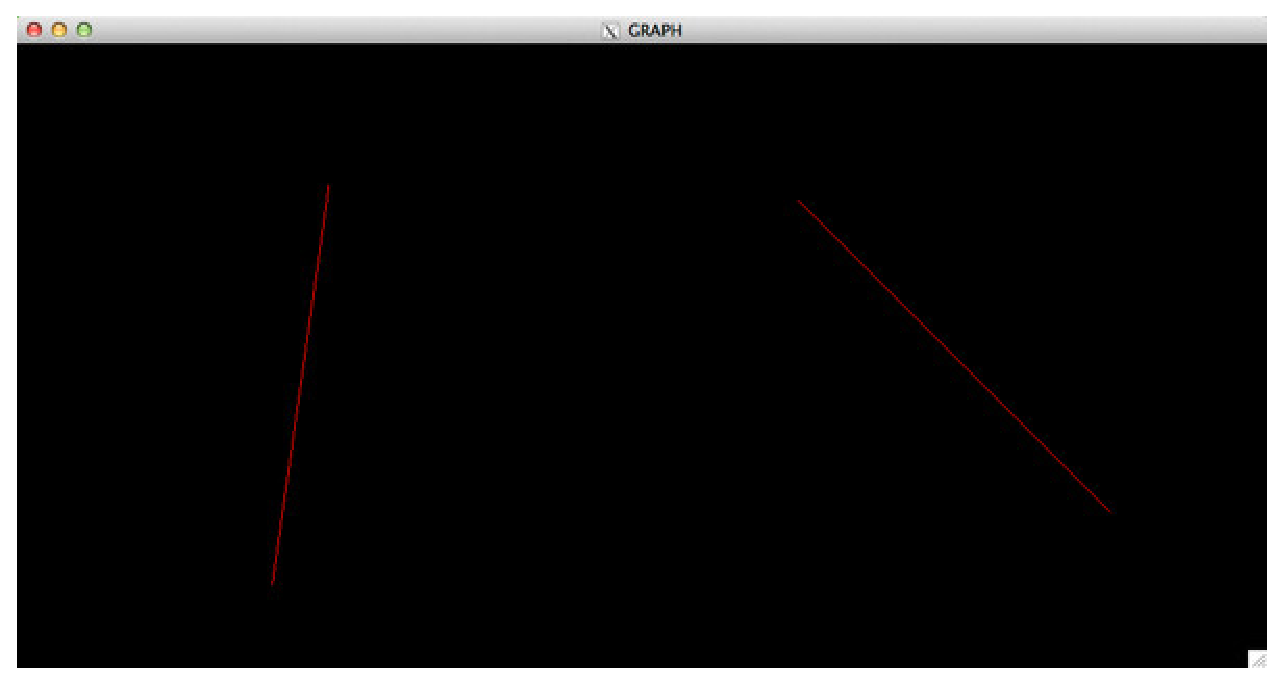
\includegraphics[width=100mm]{./Figures/eps/Canvas_g_move_g_plot.eps}
\end{figure}
%%%%%%%%%%%%%%%%%%%%%%%%%%%%%%%%%%%%%%%%%%%%%%%%%%%%%%




%%%%%%%%%%%%%%%%%%%%%g_box_2D%%%%%%%%%%%%%%%%%%%%%%%%%%%%%%
\clearpage
\subsubsection{\texttt{g\_box\_2D}}

\begin{itembox}[l]{\texttt{g\_box\_2D}関数}
%%%%%%%%%%%%%%%%%%%ここにプロトタイプ宣言を書く%%%%%%%%%%%%%%%%%%%
\begin{verbatim}
void g_box_2D(
        double x, double y,
        double width, double height,
        G_BOOL Wire, G_BOOL Fill);    
\end{verbatim}
%%%%%%%%%%%%%%%%%%%ここに引数の説明を書く%%%%%%%%%%%%%%%%%%%%%%%
\verb|x,y| ; 重心の座標\\
\verb|width,height| ; 幅と高さ\\
%\verb|WireFill| ; 塗りつぶすか(1),塗りつぶさないか(0)\\
\verb|Wire| ; \verb|G_YES|:枠線を描く, \verb|G_NO|:枠線を描かない \\
\verb|Fill| ; \verb|G_YES|:塗りつぶす, \verb|G_NO|:塗りつぶさない
\end{itembox}

%%%%%%%%%%%%%%%%%%%ここに関数の説明を書く%%%%%%%%%%%%%%%%%%%%%%%
\begin{itembox}[l]{\texttt{g\_box\_2D}関数の説明}
長方形を描画する.
\end{itembox}


%%%%%%%%%%%%%%%%%%%%%g_box_3D%%%%%%%%%%%%%%%%%%%%%%%%%%%%%%
\subsubsection{\texttt{g\_box\_3D}}

\begin{itembox}[l]{\texttt{g\_box\_3D}関数}
%%%%%%%%%%%%%%%%%%%ここにプロトタイプ宣言を書く%%%%%%%%%%%%%%%%%%%
\begin{verbatim}
void g_box_3D(
        double x, double y, double z,
        double width, double height, double depth
      	G_BOOL Wire, G_BOOL Fill);   
\end{verbatim}
%%%%%%%%%%%%%%%%%%%ここに引数の説明を書く%%%%%%%%%%%%%%%%%%%%%%%
\verb|x,y,z| ; 重心の座標\\
\verb|width,height,depth| ; 幅と高さと奥行き\\
\verb|Wire| ; \verb|G_YES|:枠線を描く, \verb|G_NO|:枠線を描かない \\
\verb|Fill| ; \verb|G_YES|:塗りつぶす, \verb|G_NO|:塗りつぶさない
\end{itembox}

%%%%%%%%%%%%%%%%%%%ここに関数の説明を書く%%%%%%%%%%%%%%%%%%%%%%%
\begin{itembox}[l]{\texttt{g\_box\_3D}関数の説明}
直方体を描画する.
\end{itembox}

%%%%%%%%%%%%%%%%%%%%%g_box_3D_core%%%%%%%%%%%%%%%%%%%%%%%%%%%%%%
\subsubsection{\texttt{g\_box\_3D\_core}}

\begin{itembox}[l]{\texttt{g\_box\_3D\_core}関数}
%%%%%%%%%%%%%%%%%%%ここにプロトタイプ宣言を書く%%%%%%%%%%%%%%%%%%%
\begin{verbatim}
void g_box_3D(
        double x, double y, double z,
        double width, double height, double depth,
        int DivideLevel,
        G_BOOL Wire, G_BOOL Fill);   
\end{verbatim}
%%%%%%%%%%%%%%%%%%%ここに引数の説明を書く%%%%%%%%%%%%%%%%%%%%%%%
\verb|x,y,z| ; 重心の座標\\
\verb|width,height,depth| ; 幅と高さと奥行き\\
\verb|DivideLevel| ;面の三角形分割レベル($4^{\verb|DivideLevel|}$倍ずつ三角形の分割数が増える)\\
%\verb|WireFill| ; \verb|G_WIRE|:ワイヤーフレーム,\ \verb|G_FILL|:塗りつぶす \\
\verb|Wire| ; \verb|G_YES|:枠線を描く, \verb|G_NO|:枠線を描かない \\
\verb|Fill| ; \verb|G_YES|:塗りつぶす, \verb|G_NO|:塗りつぶさない
\end{itembox}

%%%%%%%%%%%%%%%%%%%ここに関数の説明を書く%%%%%%%%%%%%%%%%%%%%%%%
\begin{itembox}[l]{\texttt{g\_box\_3D\_core}関数の説明}
直方体を描画する.(より細かい設定が可能)
\end{itembox}
\begin{figure}[htb]
\centering
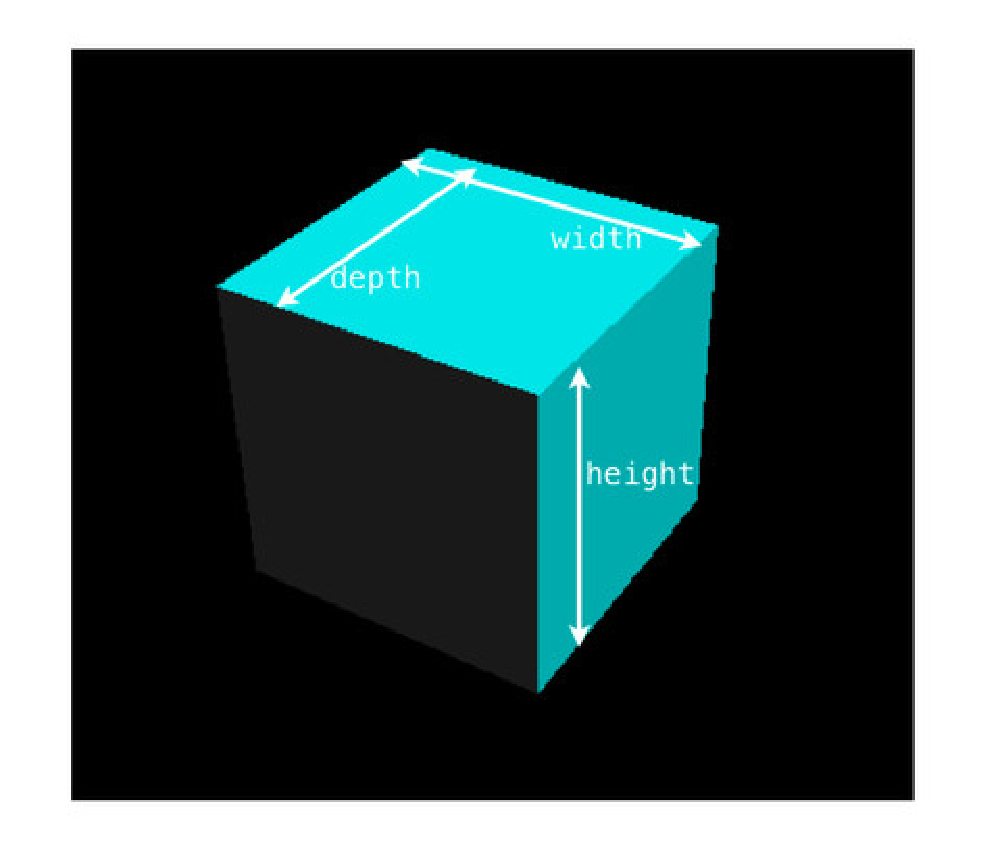
\includegraphics[width=100mm]{./Figures/eps/Canvas_g_box.eps}
\end{figure}

%%%%%%%%%%%%%%%%%%%ここに関数の説明に使う絵を載せる.%%%%%%%%%%%%%%%%
\begin{figure}[htb]
\centering
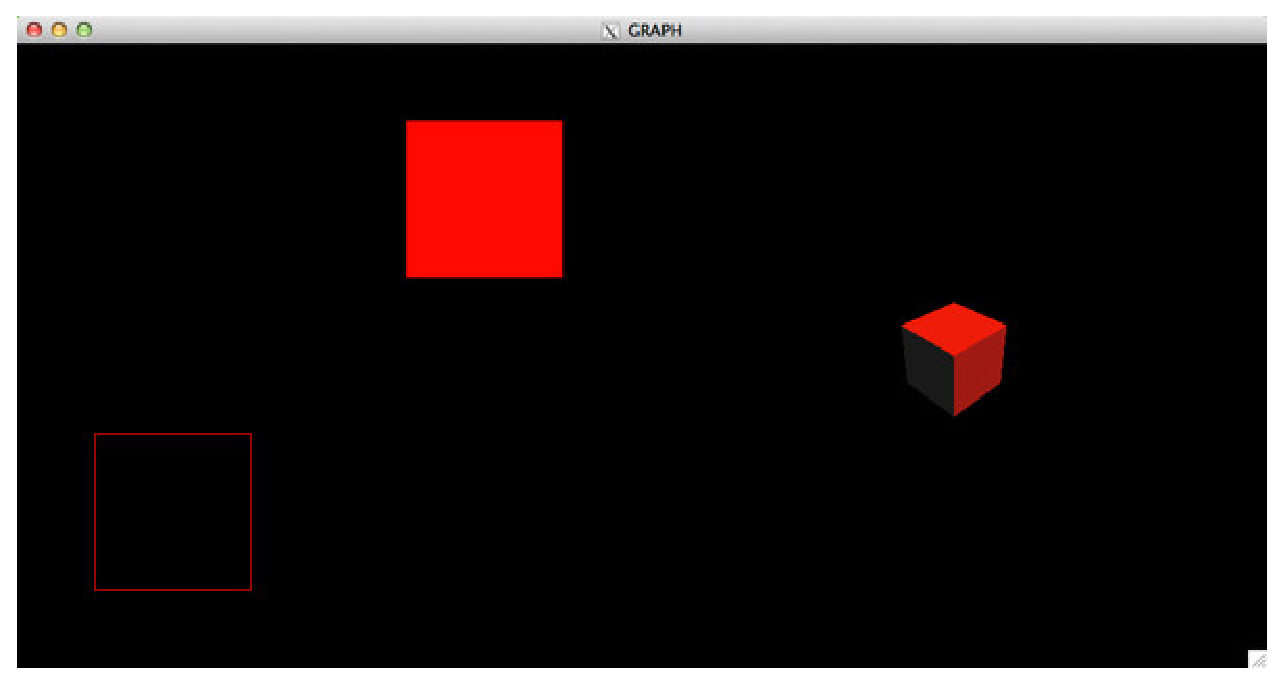
\includegraphics[width=100mm]{./Figures/eps/Canvas_g_box2.eps}
\end{figure}
%%%%%%%%%%%%%%%%%%%%%%%%%%%%%%%%%%%%%%%%%%%%%%%%%%%%%%




%%%%%%%%%%%%%%%%%%%%%g_sphere_3D%%%%%%%%%%%%%%%%%%%%%%%%%%%%%%
\clearpage
\subsubsection{\texttt{g\_sphere\_3D}}

\begin{itembox}[l]{\texttt{g\_sphere\_3D}関数}
%%%%%%%%%%%%%%%%%%%ここにプロトタイプ宣言を書く%%%%%%%%%%%%%%%%%%%
\begin{verbatim}
void g_sphere_3D(
        double x, double y, double z,
        double radius,
        G_BOOL Wire, G_BOOL Fill);   
\end{verbatim}
%%%%%%%%%%%%%%%%%%%ここに引数の説明を書く%%%%%%%%%%%%%%%%%%%%%%%
\verb|x,y,z| ; 重心の座標\\
\verb|radius| ; 半径\\
\verb|Wire| ; \verb|G_YES|:枠線を描く, \verb|G_NO|:枠線を描かない \\
\verb|Fill| ; \verb|G_YES|:塗りつぶす, \verb|G_NO|:塗りつぶさない
\end{itembox}

%%%%%%%%%%%%%%%%%%%ここに関数の説明を書く%%%%%%%%%%%%%%%%%%%%%%%
\begin{itembox}[l]{\texttt{g\_sphere\_3D}関数の説明}
球を描画する.

Ver 3.0以降: この関数を小さな球を大量に表示する目的には使用しないでください.
代わりに球マーカーを使用してください.
\end{itembox}


%%%%%%%%%%%%%%%%%%%%%g_sphere_3D_core%%%%%%%%%%%%%%%%%%%%%%%%%%%%%%
\clearpage
\subsubsection{\texttt{g\_sphere\_3D\_core}}

\begin{itembox}[l]{\texttt{g\_sphere\_3D\_core}関数}
%%%%%%%%%%%%%%%%%%%ここにプロトタイプ宣言を書く%%%%%%%%%%%%%%%%%%%
\begin{verbatim}
void g_sphere_3D_core(
        double x, double y, double z,
        double radius,
        int FaceNumberLevel, int DivideLevel, 
        G_BOOL Wire, G_BOOL Fill);   
\end{verbatim}
%%%%%%%%%%%%%%%%%%%ここに引数の説明を書く%%%%%%%%%%%%%%%%%%%%%%%
\verb|x,y,z| ; 重心の座標\\
\verb|radius| ; 半径\\
\verb|FaceNumberLevel| ; 球面の分割レベル\\
\verb|DivideLevel| ;面の三角形分割レベル($4^{\verb|DivideLevel|}$倍ずつ三角形の分割数が増える)\\
%\verb|WireFill| ; \verb|G_WIRE|:ワイヤーフレーム,\ \verb|G_FILL|:塗りつぶす \\
\verb|Wire| ; \verb|G_YES|:枠線を描く, \verb|G_NO|:枠線を描かない \\
\verb|Fill| ; \verb|G_YES|:塗りつぶす, \verb|G_NO|:塗りつぶさない
\end{itembox}

%%%%%%%%%%%%%%%%%%%ここに関数の説明を書く%%%%%%%%%%%%%%%%%%%%%%%
\begin{itembox}[l]{\texttt{g\_sphere\_3D\_core}関数の説明}
球を描画する.(より細かい設定が可能)

Ver 3.0以降: この関数を小さな球を大量に表示する目的には使用しないでください.代わりに球マーカーを使用してください.
\end{itembox}

%%%%%%%%%%%%%%%%%%%ここに関数の説明に使う絵を載せる.%%%%%%%%%%%%%%%%
\begin{figure}[htb]
\centering

\includegraphics[width=100mm]{./Figures/eps/Canvas_g_sphere_SDL.eps}
\end{figure}
%%%%%%%%%%%%%%%%%%%%%%%%%%%%%%%%%%%%%%%%%%%%%%%%%%%%%%




%%%%%%%%%%%%%%%%%%%%%g_ellipse_3D%%%%%%%%%%%%%%%%%%%%%%%%%%%%%%
\clearpage
\subsubsection{\texttt{g\_ellipse\_3D}}

\begin{itembox}[l]{\texttt{g\_ellipse\_3D}関数}
%%%%%%%%%%%%%%%%%%%ここにプロトタイプ宣言を書く%%%%%%%%%%%%%%%%%%%
\begin{verbatim}
void g_ellipse_3D(
        double x, double y, double z,
        double Sx, double Sy, double Sz,
        double direction_x, double direction_y, double direction_z,
        G_BOOL Wire, G_BOOL Fill);
\end{verbatim}
%%%%%%%%%%%%%%%%%%%ここに引数の説明を書く%%%%%%%%%%%%%%%%%%%%%%%
\verb|x,y,z| ; 重心の座標\\
\verb|Sx,Sy,Sz| ; x,y,z方向へのスケーリング率\\
\verb|direction| ; 向き\\
\verb|Wire| ; \verb|G_YES|:枠線を描く, \verb|G_NO|:枠線を描かない \\
\verb|Fill| ; \verb|G_YES|:塗りつぶす, \verb|G_NO|:塗りつぶさない
\end{itembox}

%%%%%%%%%%%%%%%%%%%ここに関数の説明を書く%%%%%%%%%%%%%%%%%%%%%%%
\begin{itembox}[l]{\texttt{g\_ellipse\_3D}関数の説明}
楕円球を描画する.
\end{itembox}

%%%%%%%%%%%%%%%%%%%ここに関数の説明に使う絵を載せる.%%%%%%%%%%%%%%%%
%%%%%%%%%%%%%%%%%%%%%%%%%%%%%%%%%%%%%%%%%%%%%%%%%%%%%%


%%%%%%%%%%%%%%%%%%%%%g_ellipse_3D_core%%%%%%%%%%%%%%%%%%%%%%%%%%%%%%
\clearpage
\subsubsection{\texttt{g\_ellipse\_3D\_core}}

\begin{itembox}[l]{\texttt{g\_ellipse\_3D\_core}関数}
%%%%%%%%%%%%%%%%%%%ここにプロトタイプ宣言を書く%%%%%%%%%%%%%%%%%%%
\begin{verbatim}
void g_ellipse_3D_core(
        double x, double y, double z,
        double Sx, double Sy, double Sz,
        double direction_x, double direction_y, double direction_z,
        int FaceNumberLevel, int DivideLevel, 
        G_BOOL Wire, G_BOOL Fill);   
\end{verbatim}
%%%%%%%%%%%%%%%%%%%ここに引数の説明を書く%%%%%%%%%%%%%%%%%%%%%%%
\verb|x,y,z| ; 重心の座標\\
\verb|Sx,Sy,Sz| ; x,y,z方向へのスケーリング率\\
\verb|direction| ; 向き\\
\verb|FaceNumberLevel| ; 球面の分割レベル\\
\verb|DivideLevel| ;面の三角形分割レベル($4^{\verb|DivideLevel|}$倍ずつ三角形の分割数が増える)\\
%\verb|WireFill| ; \verb|G_WIRE|:ワイヤーフレーム,\ \verb|G_FILL|:塗りつぶす \\
\verb|Wire| ; \verb|G_YES|:枠線を描く, \verb|G_NO|:枠線を描かない \\
\verb|Fill| ; \verb|G_YES|:塗りつぶす, \verb|G_NO|:塗りつぶさない
\end{itembox}

%%%%%%%%%%%%%%%%%%%ここに関数の説明を書く%%%%%%%%%%%%%%%%%%%%%%%
\begin{itembox}[l]{\texttt{g\_ellipse\_3D\_core}関数の説明}
楕円球を描画する.(より細かい設定が可能)
\end{itembox}

%%%%%%%%%%%%%%%%%%%ここに関数の説明に使う絵を載せる.%%%%%%%%%%%%%%%%
\begin{figure}[htb]
\centering
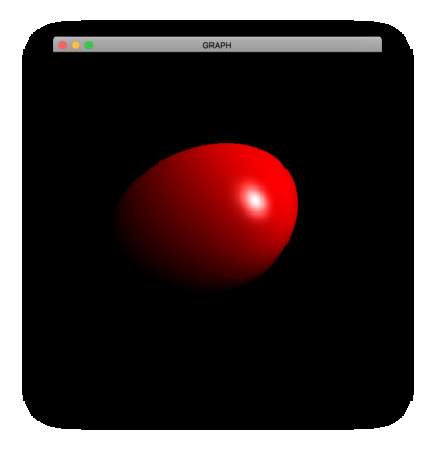
\includegraphics[width=100mm]{./Figures/eps/Canvas_g_ellipse_SDL.eps}
\end{figure}
%%%%%%%%%%%%%%%%%%%%%%%%%%%%%%%%%%%%%%%%%%%%%%%%%%%%%%




%%%%%%%%%%%%%%%%%%%%%g_prism_3D%%%%%%%%%%%%%%%%%%%%%%%%%%%%%%
\clearpage
\subsubsection{\texttt{g\_prism\_3D}}

\begin{itembox}[l]{\texttt{g\_prism\_3D}関数}
%%%%%%%%%%%%%%%%%%%ここにプロトタイプ宣言を書く%%%%%%%%%%%%%%%%%%%
\begin{verbatim}
void g_prism_3D(
        double center_x, double center_y, double center_z,
        double direction_x, double direction_y, double direction_z,
        double radius, double height, double psi, int N,
        G_BOOL Wire, G_BOOL Fill);   
\end{verbatim}
%%%%%%%%%%%%%%%%%%%ここに引数の説明を書く%%%%%%%%%%%%%%%%%%%%%%%
\verb|center| ; 重心の座標\\
\verb|direction| ; 向き\\
\verb|radius| ; 半径\\
\verb|height| ; 高さ\\
\verb|psi| ; \verb|direction|に対する回転角\\
\verb|N| ; 側面の数\\
\verb|Wire| ; \verb|G_YES|:枠線を描く, \verb|G_NO|:枠線を描かない \\
\verb|Fill| ; \verb|G_YES|:塗りつぶす, \verb|G_NO|:塗りつぶさない
\end{itembox}

%%%%%%%%%%%%%%%%%%%ここに関数の説明を書く%%%%%%%%%%%%%%%%%%%%%%%
\begin{itembox}[l]{\texttt{g\_prism\_3D}関数の説明}
角柱を描画する.
\end{itembox}

%%%%%%%%%%%%%%%%%%%ここに関数の説明に使う絵を載せる.%%%%%%%%%%%%%%%%
%%%%%%%%%%%%%%%%%%%%%%%%%%%%%%%%%%%%%%%%%%%%%%%%%%%%%%




%%%%%%%%%%%%%%%%%%%%%g_prism_3D_core%%%%%%%%%%%%%%%%%%%%%%%%%%%%%%
\clearpage
\subsubsection{\texttt{g\_prism\_3D\_core}}

\begin{itembox}[l]{\texttt{g\_prism\_3D\_core}関数}
%%%%%%%%%%%%%%%%%%%ここにプロトタイプ宣言を書く%%%%%%%%%%%%%%%%%%%
\begin{verbatim}
void g_prism_3D_core(
        double center_x, double center_y, double center_z,
        double direction_x, double direction_y, double direction_z,
        double radius, double height, double psi, int N,
        int DivideLevel, G_BOOL Wire, G_BOOL Fill);   
\end{verbatim}
%%%%%%%%%%%%%%%%%%%ここに引数の説明を書く%%%%%%%%%%%%%%%%%%%%%%%
\verb|center| ; 重心の座標\\
\verb|direction| ; 向き\\
\verb|radius| ; 半径\\
\verb|height| ; 高さ\\
\verb|psi| ; \verb|direction|に対する回転角\\
\verb|N| ; 側面の数\\
\verb|DivideLevel| ;面の三角形分割レベル($4^{\verb|DivideLevel|}$倍ずつ三角形の分割数が増える)\\
%\verb|WireFill| ; \verb|G_WIRE|:ワイヤーフレーム,\ \verb|G_FILL|:塗りつぶす \\
\verb|Wire| ; \verb|G_YES|:枠線を描く, \verb|G_NO|:枠線を描かない \\
\verb|Fill| ; \verb|G_YES|:塗りつぶす, \verb|G_NO|:塗りつぶさない
\end{itembox}

%%%%%%%%%%%%%%%%%%%ここに関数の説明を書く%%%%%%%%%%%%%%%%%%%%%%%
\begin{itembox}[l]{\texttt{g\_prism\_3D\_core}関数の説明}
角柱を描画する.(より細かい設定が可能)
\end{itembox}

%%%%%%%%%%%%%%%%%%%ここに関数の説明に使う絵を載せる.%%%%%%%%%%%%%%%%
\begin{figure}[htb]
\centering
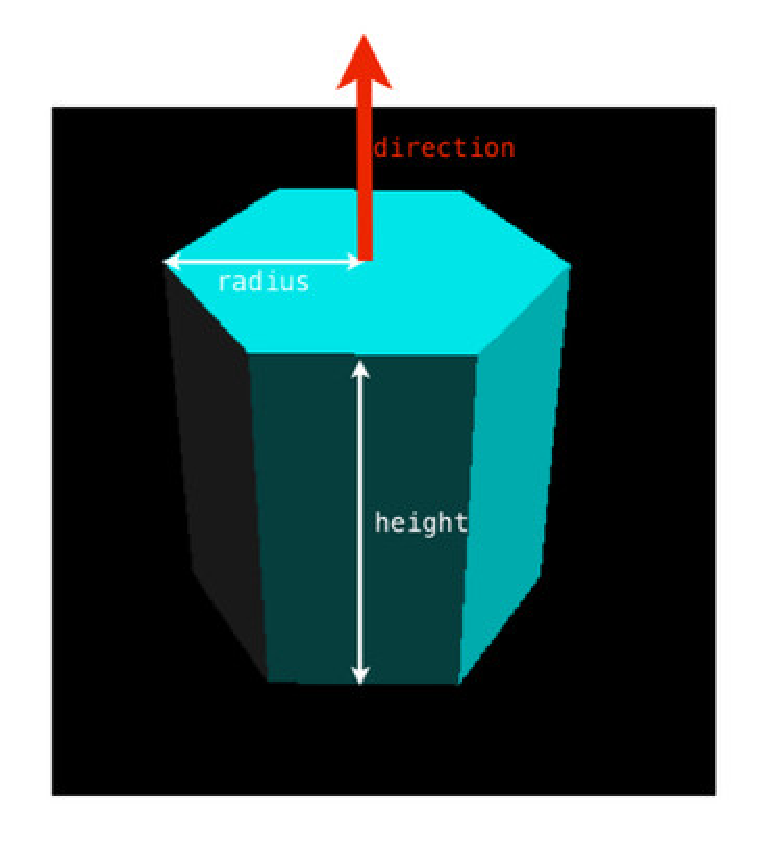
\includegraphics[width=100mm]{./Figures/eps/Canvas_g_prism.eps}
\end{figure}
%%%%%%%%%%%%%%%%%%%%%%%%%%%%%%%%%%%%%%%%%%%%%%%%%%%%%%




%%%%%%%%%%%%%%%%%%%%%g_cylinder_3D%%%%%%%%%%%%%%%%%%%%%%%%%%%%%%
\clearpage
\subsubsection{\texttt{g\_cylinder\_3D}}

\begin{itembox}[l]{\texttt{g\_cylinder\_3D}関数}
%%%%%%%%%%%%%%%%%%%ここにプロトタイプ宣言を書く%%%%%%%%%%%%%%%%%%%
\begin{verbatim}
void g_cylinder_3D(
        double center_x, double center_y, double center_z,
        double direction_x, double direction_y, double direction_z,
        double radius, double height, double psi,
        G_BOOL Wire, G_BOOL Fill);   
\end{verbatim}
%%%%%%%%%%%%%%%%%%%ここに引数の説明を書く%%%%%%%%%%%%%%%%%%%%%%%
\verb|center| ; 重心の座標\\
\verb|direction| ; 向き\\
\verb|radius| ; 半径\\
\verb|height| ; 高さ\\
\verb|psi| ; \verb|direction|に対する回転角\\
\verb|Wire| ; \verb|G_YES|:枠線を描く, \verb|G_NO|:枠線を描かない \\
\verb|Fill| ; \verb|G_YES|:塗りつぶす, \verb|G_NO|:塗りつぶさない
\end{itembox}

%%%%%%%%%%%%%%%%%%%ここに関数の説明を書く%%%%%%%%%%%%%%%%%%%%%%%
\begin{itembox}[l]{\texttt{g\_cylinder\_3D}関数の説明}
円柱を描画する.
\end{itembox}

%%%%%%%%%%%%%%%%%%%ここに関数の説明に使う絵を載せる.%%%%%%%%%%%%%%%%
%%%%%%%%%%%%%%%%%%%%%%%%%%%%%%%%%%%%%%%%%%%%%%%%%%%%%%


%%%%%%%%%%%%%%%%%%%%%g_cylinder_3D_core%%%%%%%%%%%%%%%%%%%%%%%%%%%%%%
\clearpage
\subsubsection{\texttt{g\_cylinder\_3D\_core}}

\begin{itembox}[l]{\texttt{g\_cylinder\_3D\_core}関数}
%%%%%%%%%%%%%%%%%%%ここにプロトタイプ宣言を書く%%%%%%%%%%%%%%%%%%%
\begin{verbatim}
void g_cylinder_3D_core(
        double center_x, double center_y, double center_z,
        double direction_x, double direction_y, double direction_z,
        double radius, double height, double psi,
        int N, int DivideLevel, 
        G_BOOL Wire, G_BOOL Fill);   
\end{verbatim}
%%%%%%%%%%%%%%%%%%%ここに引数の説明を書く%%%%%%%%%%%%%%%%%%%%%%%
\verb|center| ; 重心の座標\\
\verb|direction| ; 向き\\
\verb|radius| ; 半径\\
\verb|height| ; 高さ\\
\verb|psi| ; \verb|direction|に対する回転角\\
\verb|N| ; 側面の数\\
\verb|DivideLevel| ;面の三角形分割レベル($4^{\verb|DivideLevel|}$倍ずつ三角形の分割数が増える)\\
%\verb|WireFill| ; \verb|G_WIRE|:ワイヤーフレーム,\ \verb|G_FILL|:塗りつぶす \\
\verb|Wire| ; \verb|G_YES|:枠線を描く, \verb|G_NO|:枠線を描かない \\
\verb|Fill| ; \verb|G_YES|:塗りつぶす, \verb|G_NO|:塗りつぶさない
\end{itembox}

%%%%%%%%%%%%%%%%%%%ここに関数の説明を書く%%%%%%%%%%%%%%%%%%%%%%%
\begin{itembox}[l]{\texttt{g\_cylinder\_3D\_core}関数の説明}
円柱を描画する.(より細かい設定が可能)
\end{itembox}

%%%%%%%%%%%%%%%%%%%ここに関数の説明に使う絵を載せる.%%%%%%%%%%%%%%%%
\begin{figure}[htb]
\centering
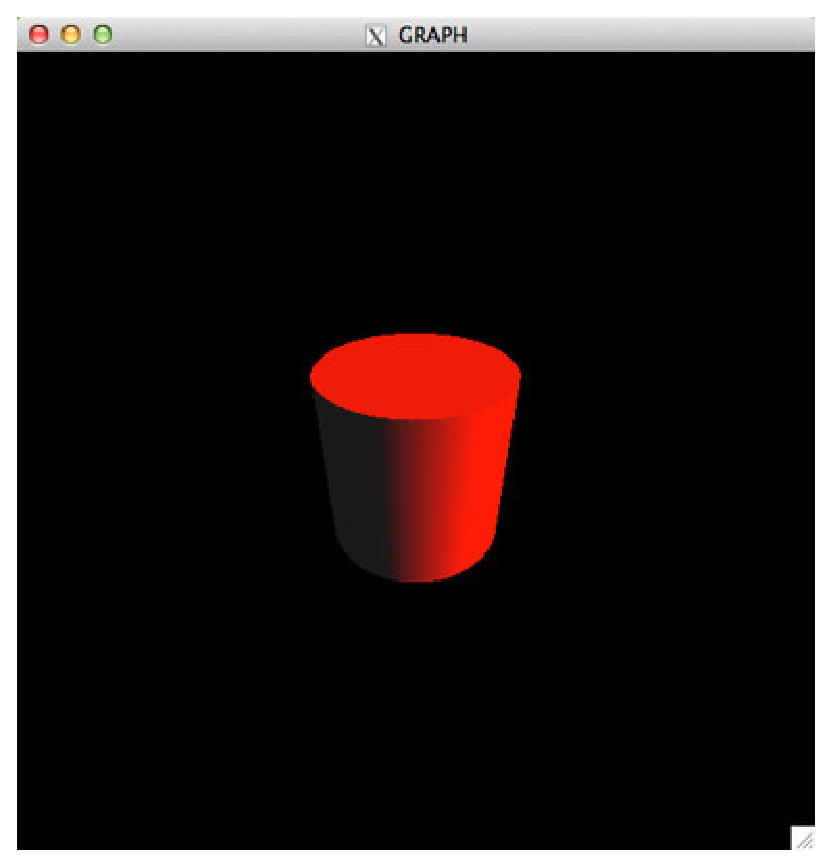
\includegraphics[width=100mm]{./Figures/eps/Canvas_g_cylinder.eps}
\end{figure}
%%%%%%%%%%%%%%%%%%%%%%%%%%%%%%%%%%%%%%%%%%%%%%%%%%%%%%




%%%%%%%%%%%%%%%%%%%%%%%g_cone_2D%%%%%%%%%%%%%%%%%%%%%%%%%%%%%%
%%\clearpage
%%\subsubsection{\texttt{g\_cone\_2D}}
%%
%%\begin{itembox}[l]{\texttt{g\_cone\_2D}関数}
%%%%%%%%%%%%%%%%%%%%%ここにプロトタイプ宣言を書く%%%%%%%%%%%%%%%%%%%
%%\begin{verbatim}
%%void g_cone_2D(
%%        double center_x, double center_y,
%%        double direction_x, double direction_y,
%%        double radius, double head_size, int type);
%%\end{verbatim}
%%%%%%%%%%%%%%%%%%%%%ここに引数の説明を書く%%%%%%%%%%%%%%%%%%%%%%%
%%\verb|center| ; 重心の座標\\
%%\verb|direction| ; 向き\\
%%\verb|radius| ; 半径\\
%%\verb|head_size| ; 高さ\\
%%\verb|type| ; 種類(0〜2)\\
%%\end{itembox}
%%
%%%%%%%%%%%%%%%%%%%%%ここに関数の説明を書く%%%%%%%%%%%%%%%%%%%%%%%
%%\begin{itembox}[l]{\texttt{g\_cone\_2D}関数の説明}
%%二等辺三角形を描画する.
%%\end{itembox}
%%
%%%%%%%%%%%%%%%%%%%%%ここに関数の説明に使う絵を載せる.%%%%%%%%%%%%%%%%
%%\begin{figure}[htb]
%%\end{figure}
%%%%%%%%%%%%%%%%%%%%%%%%%%%%%%%%%%%%%%%%%%%%%%%%%%%%%%%%




%%%%%%%%%%%%%%%%%%%%%g_cone_3D%%%%%%%%%%%%%%%%%%%%%%%%%%%%%%
\clearpage
\subsubsection{\texttt{g\_cone\_3D}}

\begin{itembox}[l]{\texttt{g\_cone\_3D}関数}
%%%%%%%%%%%%%%%%%%%ここにプロトタイプ宣言を書く%%%%%%%%%%%%%%%%%%%
\begin{verbatim}
void g_cone_3D(
        double center_x, double center_y, double center_z,
        double direction_x, double direction_y, double direction_z,
        double radius, double head_size
        G_BOOL Wire, G_BOOL Fill);
\end{verbatim}
%%%%%%%%%%%%%%%%%%%ここに引数の説明を書く%%%%%%%%%%%%%%%%%%%%%%%
\verb|center| ; 重心の座標\\
\verb|direction| ; 向き\\
\verb|radius| ; 半径\\
\verb|head_size| ; 高さ\\
\verb|Wire| ; \verb|G_YES|:枠線を描く, \verb|G_NO|:枠線を描かない \\
\verb|Fill| ; \verb|G_YES|:塗りつぶす, \verb|G_NO|:塗りつぶさない
\end{itembox}

%%%%%%%%%%%%%%%%%%%ここに関数の説明を書く%%%%%%%%%%%%%%%%%%%%%%%
\begin{itembox}[l]{\texttt{g\_cone\_3D}関数の説明}
円錐を描画する.
\end{itembox}
\begin{figure}[htb]
\centering
	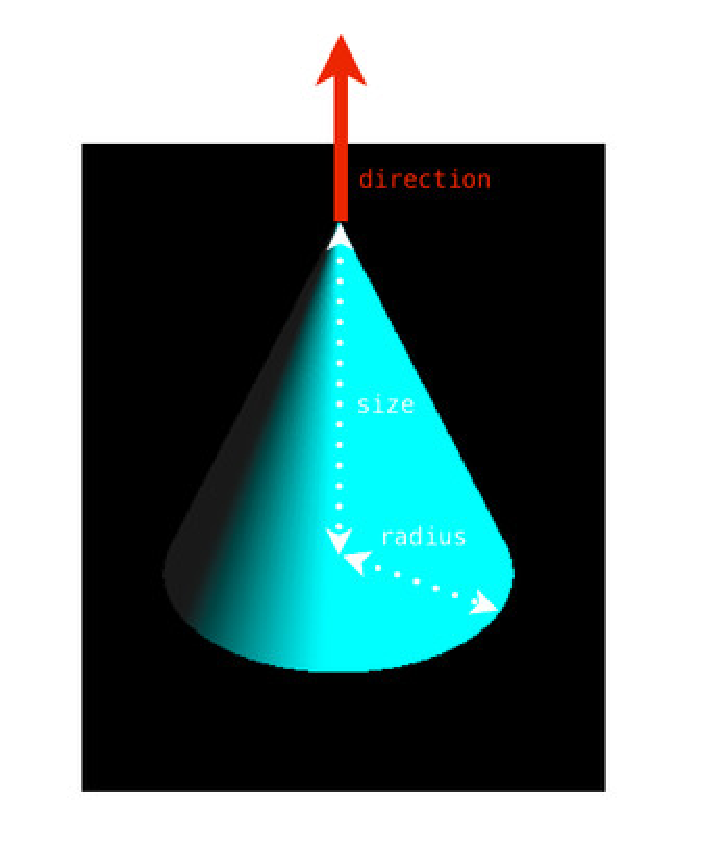
\includegraphics[width=100mm]{./Figures/eps/Canvas_g_cone.eps}
\end{figure}

%%%%%%%%%%%%%%%%%%%ここに関数の説明に使う絵を載せる.%%%%%%%%%%%%%%%%
%%%%%%%%%%%%%%%%%%%%%%%%%%%%%%%%%%%%%%%%%%%%%%%%%%%%%%


%%%%%%%%%%%%%%%%%%%%%g_cone_3D_core%%%%%%%%%%%%%%%%%%%%%%%%%%%%%%
\clearpage
\subsubsection{\texttt{g\_cone\_3D\_core}}

\begin{itembox}[l]{\texttt{g\_cone\_3D\_core}関数}
%%%%%%%%%%%%%%%%%%%ここにプロトタイプ宣言を書く%%%%%%%%%%%%%%%%%%%
\begin{verbatim}
void g_cone_3D_core(
        double center_x, double center_y, double center_z,
        double direction_x, double direction_y, double direction_z,
        double radius, double head_size,
        int N, int DivideLevel, 
        G_BOOL Wire, G_BOOL Fill);
\end{verbatim}
%%%%%%%%%%%%%%%%%%%ここに引数の説明を書く%%%%%%%%%%%%%%%%%%%%%%%
\verb|center| ; 重心の座標\\
\verb|direction| ; 向き\\
\verb|radius| ; 半径\\
\verb|head_size| ; 高さ\\
\verb|N| ; 円周の分割数\\
\verb|DivideLevel| ;面の三角形分割レベル($4^{\verb|DivideLevel|}$倍ずつ三角形の分割数が増える)\\
\verb|Wire| ; \verb|G_YES|:枠線を描く, \verb|G_NO|:枠線を描かない \\
\verb|Fill| ; \verb|G_YES|:塗りつぶす, \verb|G_NO|:塗りつぶさない 
\end{itembox}

%%%%%%%%%%%%%%%%%%%ここに関数の説明を書く%%%%%%%%%%%%%%%%%%%%%%%
\begin{itembox}[l]{\texttt{g\_cone\_3D\_core}関数の説明}
円錐を描画する.(より細かい設定が可能)
\end{itembox}
\begin{figure}[htb]
\centering
	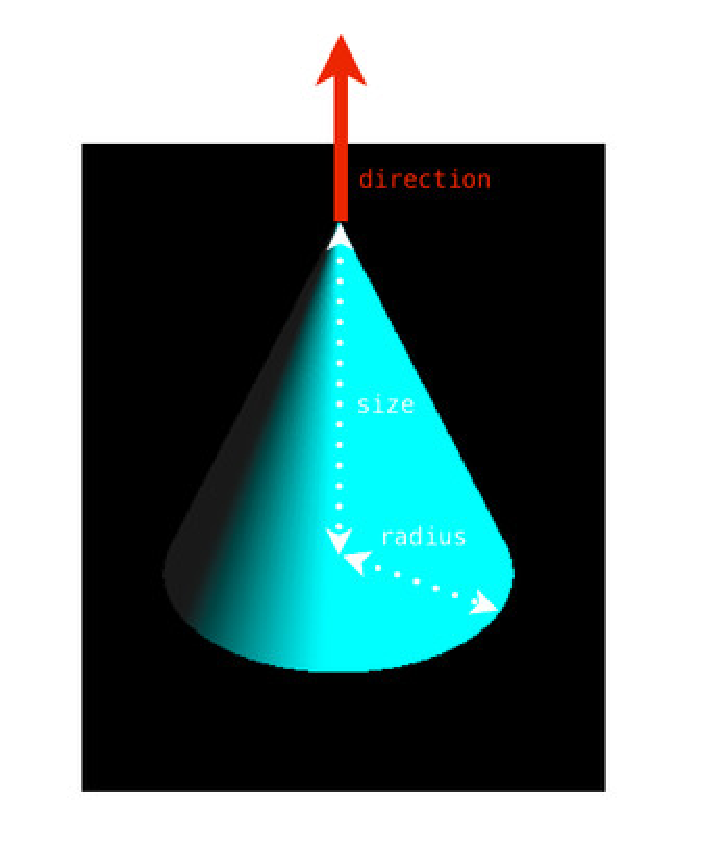
\includegraphics[width=100mm]{./Figures/eps/Canvas_g_cone.eps}
\end{figure}

%%%%%%%%%%%%%%%%%%%ここに関数の説明に使う絵を載せる.%%%%%%%%%%%%%%%%
\begin{figure}[htb]
\centering
	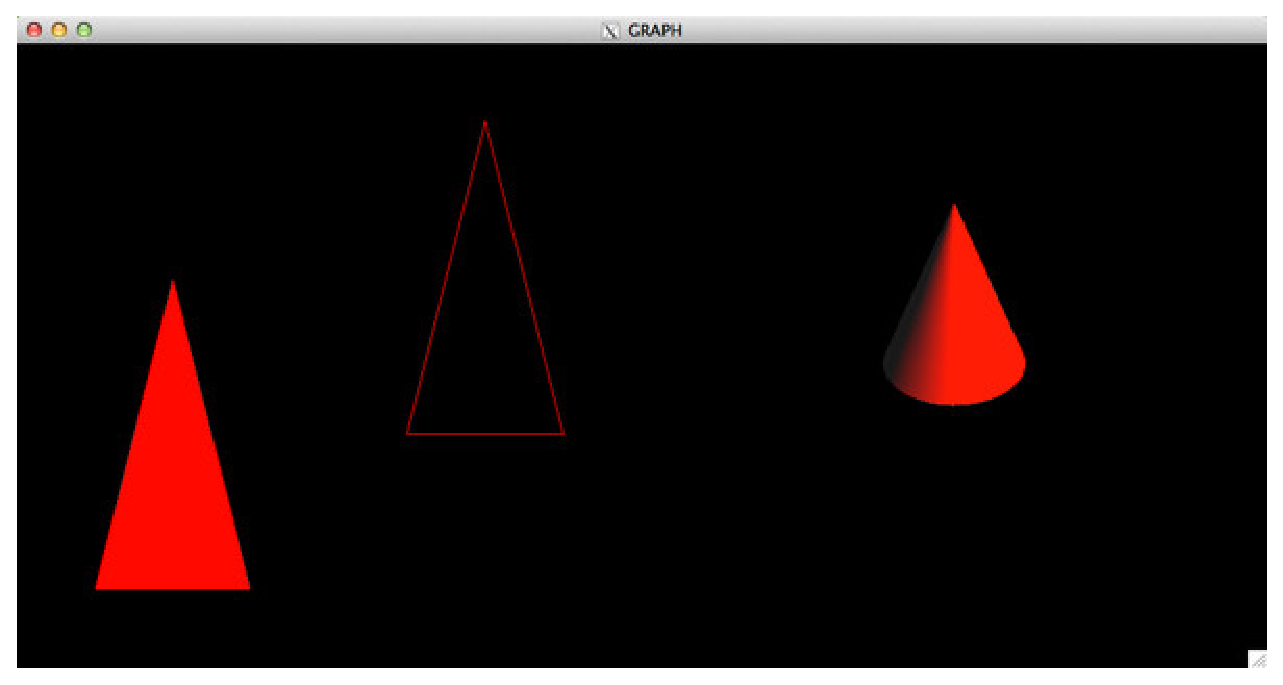
\includegraphics[width=100mm]{./Figures/eps/Canvas_g_cone2.eps}
\end{figure}
%%%%%%%%%%%%%%%%%%%%%%%%%%%%%%%%%%%%%%%%%%%%%%%%%%%%%%




%%%%%%%%%%%%%%%%%%%%%g_pyramid_3D%%%%%%%%%%%%%%%%%%%%%%%%%%%%%%
\clearpage
\subsubsection{\texttt{g\_pyramid\_3D}}

\begin{itembox}[l]{\texttt{g\_pyramid\_3D}関数}
%%%%%%%%%%%%%%%%%%%ここにプロトタイプ宣言を書く%%%%%%%%%%%%%%%%%%%
\begin{verbatim}
void g_pyramid_3D(
        double center_x, double center_y, double center_z,
        double direction_x, double direction_y, double direction_z,
        double radius, double head_size, double psi, int N,
        G_BOOL Wire, G_BOOL Fill);
\end{verbatim}
%%%%%%%%%%%%%%%%%%%ここに引数の説明を書く%%%%%%%%%%%%%%%%%%%%%%%
\verb|center| ; 重心の座標\\
\verb|direction| ; 向き\\
\verb|radius| ; 半径\\
\verb|head_size| ; 高さ\\
\verb|psi| ; \verb|direction|に対する回転角\\
\verb|N| ; 側面の数\\
\verb|Wire| ; \verb|G_YES|:枠線を描く, \verb|G_NO|:枠線を描かない \\
\verb|Fill| ; \verb|G_YES|:塗りつぶす, \verb|G_NO|:塗りつぶさない 
\end{itembox}

%%%%%%%%%%%%%%%%%%%ここに関数の説明を書く%%%%%%%%%%%%%%%%%%%%%%%
\begin{itembox}[l]{\texttt{g\_pyramid\_3D}関数の説明}
角錐を描画する.
\end{itembox}

%%%%%%%%%%%%%%%%%%%ここに関数の説明に使う絵を載せる.%%%%%%%%%%%%%%%%
%%%%%%%%%%%%%%%%%%%%%%%%%%%%%%%%%%%%%%%%%%%%%%%%%%%%%%


%%%%%%%%%%%%%%%%%%%%%g_pyramid_3D_core%%%%%%%%%%%%%%%%%%%%%%%%%%%%%%
\clearpage
\subsubsection{\texttt{g\_pyramid\_3D\_core}}

\begin{itembox}[l]{\texttt{g\_pyramid\_3D\_core}関数}
%%%%%%%%%%%%%%%%%%%ここにプロトタイプ宣言を書く%%%%%%%%%%%%%%%%%%%
\begin{verbatim}
void g_pyramid_3D_core(
        double center_x, double center_y, double center_z,
        double direction_x, double direction_y, double direction_z,
        double radius, double head_size, double psi, int N,
        int DivideLevel, G_BOOL Wire, G_BOOL Fill);
\end{verbatim}
%%%%%%%%%%%%%%%%%%%ここに引数の説明を書く%%%%%%%%%%%%%%%%%%%%%%%
\verb|center| ; 重心の座標\\
\verb|direction| ; 向き\\
\verb|radius| ; 半径\\
\verb|head_size| ; 高さ\\
\verb|psi| ; \verb|direction|に対する回転角\\
\verb|N| ; 側面の数\\
\verb|DivideLevel| ;面の三角形分割レベル($4^{\verb|DivideLevel|}$倍ずつ三角形の分割数が増える)\\
%\verb|WireFill| ; \verb|G_WIRE|:ワイヤーフレーム,\ \verb|G_FILL|:塗りつぶす \\
\verb|Wire| ; \verb|G_YES|:枠線を描く, \verb|G_NO|:枠線を描かない \\
\verb|Fill| ; \verb|G_YES|:塗りつぶす, \verb|G_NO|:塗りつぶさない 
\end{itembox}

%%%%%%%%%%%%%%%%%%%ここに関数の説明を書く%%%%%%%%%%%%%%%%%%%%%%%
\begin{itembox}[l]{\texttt{g\_pyramid\_3D\_core}関数の説明}
角錐を描画する.(より細かい設定が可能)
\end{itembox}

%%%%%%%%%%%%%%%%%%%ここに関数の説明に使う絵を載せる.%%%%%%%%%%%%%%%%
\begin{figure}[htb]
\centering
	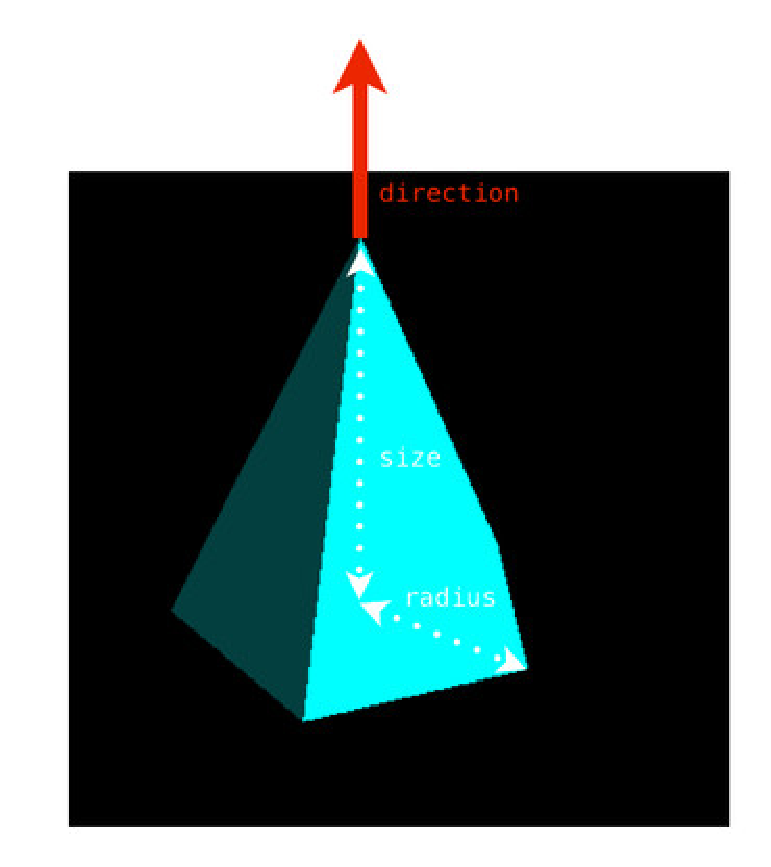
\includegraphics[width=100mm]{./Figures/eps/Canvas_g_pyramid.eps}
\end{figure}
%%%%%%%%%%%%%%%%%%%%%%%%%%%%%%%%%%%%%%%%%%%%%%%%%%%%%%




%%%%%%%%%%%%%%%%%%%%%g_arrow_2D%%%%%%%%%%%%%%%%%%%%%%%%%%%%%%
\clearpage
\subsubsection{\texttt{g\_arrow\_2D}}

\begin{itembox}[l]{\texttt{g\_arrow\_2D}関数}
%%%%%%%%%%%%%%%%%%%ここにプロトタイプ宣言を書く%%%%%%%%%%%%%%%%%%%
\begin{verbatim}
void g_arrow_2D(
        double base_x, double base_y
        double direction_x, double direction_y
        double arrow_size, double head_size, int type);
\end{verbatim}
%%%%%%%%%%%%%%%%%%%ここに引数の説明を書く%%%%%%%%%%%%%%%%%%%%%%%
\verb|base| ; 根元の座標\\
\verb|direction| ; 向き\\
\verb|arrow_size| ; 全体の長さ\\
\verb|head_size| ; 傘の部分の長さ\\
\verb|type| ; 矢印の種類(0〜2)
\end{itembox}

%%%%%%%%%%%%%%%%%%%ここに関数の説明を書く%%%%%%%%%%%%%%%%%%%%%%%
\begin{itembox}[l]{\texttt{g\_arrow\_2D}関数の説明}
矢印を描画する.
\end{itembox}

%%%%%%%%%%%%%%%%%%%ここに関数の説明に使う絵を載せる.%%%%%%%%%%%%%%%%
\begin{figure}[htb]
\end{figure}
%%%%%%%%%%%%%%%%%%%%%%%%%%%%%%%%%%%%%%%%%%%%%%%%%%%%%%


%%%%%%%%%%%%%%%%%%%%%g_arrow_3D%%%%%%%%%%%%%%%%%%%%%%%%%%%%%%
\clearpage
\subsubsection{\texttt{g\_arrow\_3D}}

\begin{itembox}[l]{\texttt{g\_arrow\_3D}関数}
%%%%%%%%%%%%%%%%%%%ここにプロトタイプ宣言を書く%%%%%%%%%%%%%%%%%%%
\begin{verbatim}
void g_arrow_3D(
        double base_x, double base_y, double base_z,
        double direction_x, double direction_y, double direction_z,
        double arrow_size, double head_size,
        G_BOOL Wire, G_BOOL Fill);
\end{verbatim}
%%%%%%%%%%%%%%%%%%%ここに引数の説明を書く%%%%%%%%%%%%%%%%%%%%%%%
\verb|base| ; 根元の座標\\
\verb|direction| ; 向き\\
\verb|arrow_size| ; 全体の長さ\\
\verb|head_size| ; 傘の部分の長さ\\
\verb|Wire| ; \verb|G_YES|:枠線を描く, \verb|G_NO|:枠線を描かない \\
\verb|Fill| ; \verb|G_YES|:塗りつぶす, \verb|G_NO|:塗りつぶさない 
\end{itembox}

%%%%%%%%%%%%%%%%%%%ここに関数の説明を書く%%%%%%%%%%%%%%%%%%%%%%%
\begin{itembox}[l]{\texttt{g\_arrow\_3D}関数の説明}
矢印を描画する.
\end{itembox}
\begin{figure}[htb]
\centering
	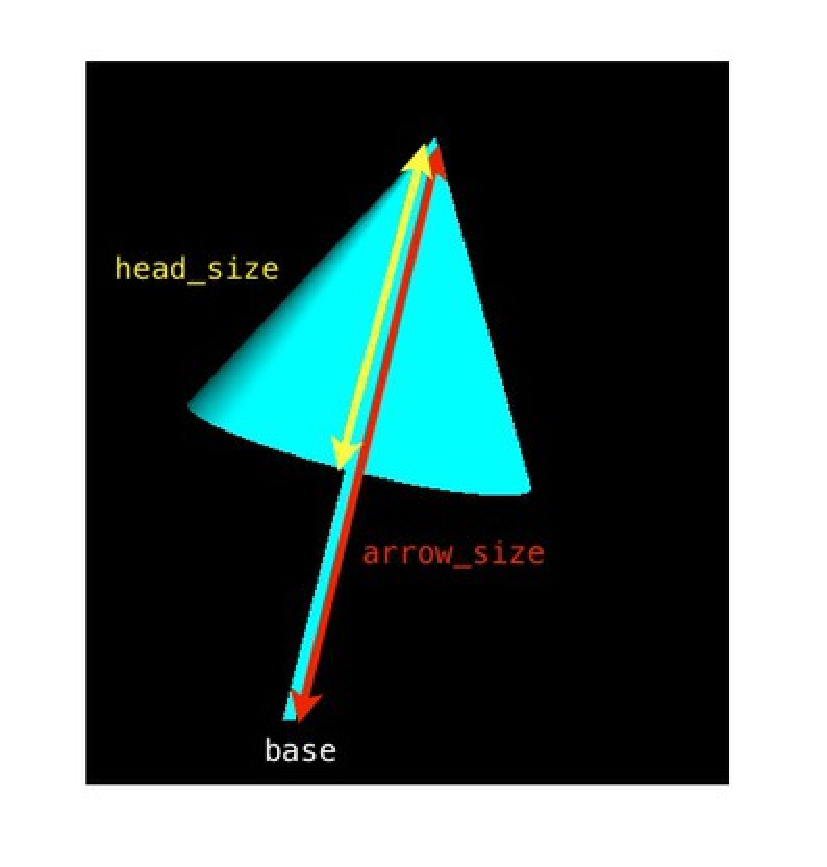
\includegraphics[width=100mm]{./Figures/eps/Canvas_g_arrow.eps}
\end{figure}

%%%%%%%%%%%%%%%%%%%ここに関数の説明に使う絵を載せる.%%%%%%%%%%%%%%%%
%%%%%%%%%%%%%%%%%%%%%%%%%%%%%%%%%%%%%%%%%%%%%%%%%%%%%%


%%%%%%%%%%%%%%%%%%%%%g_arrow_3D_core%%%%%%%%%%%%%%%%%%%%%%%%%%%%%%
\clearpage
\subsubsection{\texttt{g\_arrow\_3D\_core}}

\begin{itembox}[l]{\texttt{g\_arrow\_3D\_core}関数}
%%%%%%%%%%%%%%%%%%%ここにプロトタイプ宣言を書く%%%%%%%%%%%%%%%%%%%
\begin{verbatim}
void g_arrow_3D_core(
        double base_x, double base_y, double base_z,
        double direction_x, double direction_y, double direction_z,
        double arrow_size, double head_size, 
        int N, int DivideLevel, 
        G_BOOL Wire, G_BOOL Fill);
\end{verbatim}
%%%%%%%%%%%%%%%%%%%ここに引数の説明を書く%%%%%%%%%%%%%%%%%%%%%%%
\verb|base| ; 根元の座標\\
\verb|direction| ; 向き\\
\verb|arrow_size| ; 全体の長さ\\
\verb|head_size| ; 傘の部分の長さ\\
\verb|N| ; 傘の部分の分割数\\
\verb|DivideLevel| ;面の三角形分割レベル($4^{\verb|DivideLevel|}$倍ずつ三角形の分割数が増える)\\
%\verb|WireFill| ; \verb|G_WIRE|:ワイヤーフレーム,\ \verb|G_FILL|:塗りつぶす \\
\verb|Wire| ; \verb|G_YES|:枠線を描く, \verb|G_NO|:枠線を描かない \\
\verb|Fill| ; \verb|G_YES|:塗りつぶす, \verb|G_NO|:塗りつぶさない 
\end{itembox}

%%%%%%%%%%%%%%%%%%%ここに関数の説明を書く%%%%%%%%%%%%%%%%%%%%%%%
\begin{itembox}[l]{\texttt{g\_arrow\_3D\_core}関数の説明}
矢印を描画する.(より細かい設定が可能)
\end{itembox}
\begin{figure}[htb]
\centering
	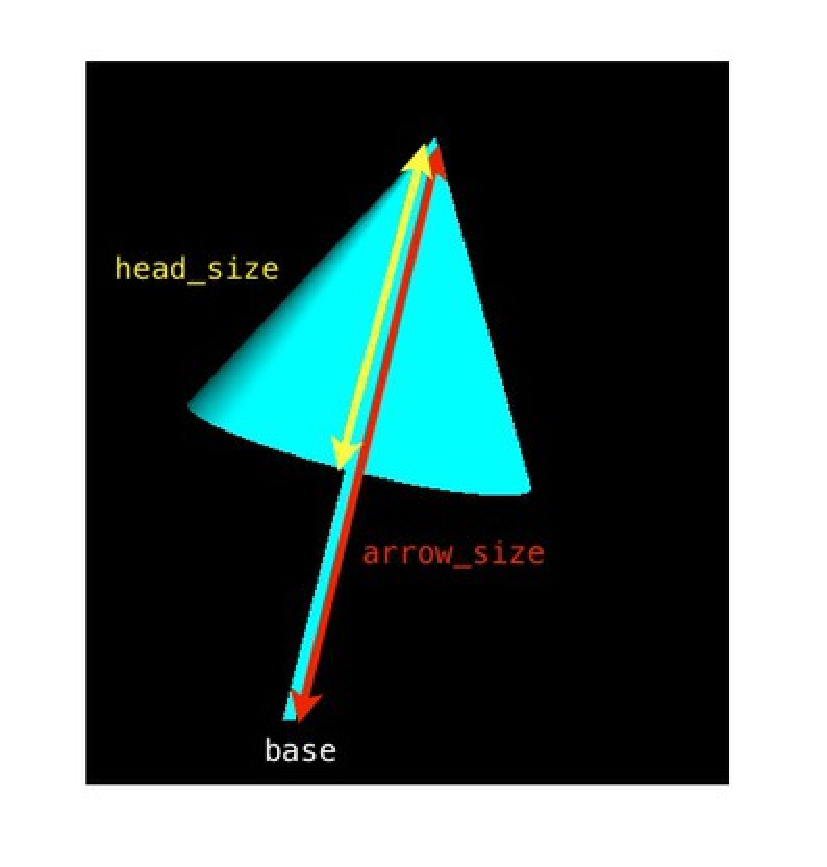
\includegraphics[width=100mm]{./Figures/eps/Canvas_g_arrow.eps}
\end{figure}

%%%%%%%%%%%%%%%%%%%ここに関数の説明に使う絵を載せる.%%%%%%%%%%%%%%%%
\begin{figure}[htb]
\centering
	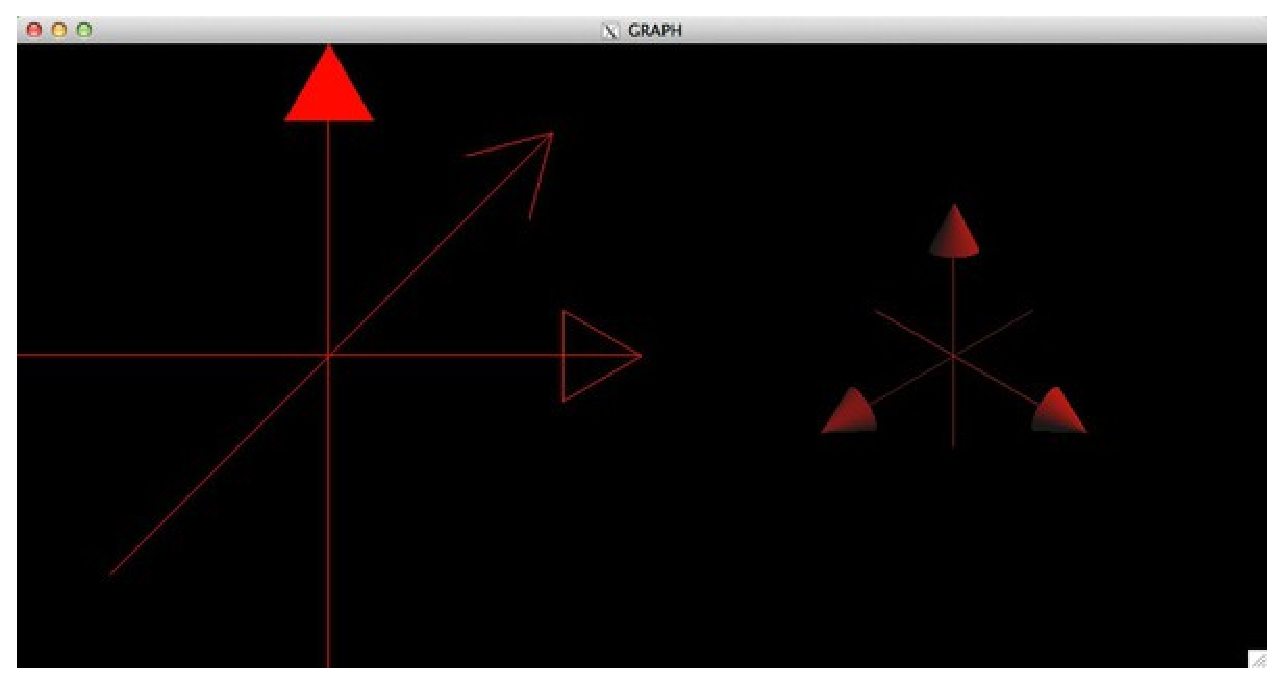
\includegraphics[width=100mm]{./Figures/eps/Canvas_g_arrow2.eps}
\end{figure}
%%%%%%%%%%%%%%%%%%%%%%%%%%%%%%%%%%%%%%%%%%%%%%%%%%%%%%




%%%%%%%%%%%%%%%%%%%%%g_triangle_2D%%%%%%%%%%%%%%%%%%%%%%%%%%%%%%
\clearpage
\subsubsection{\texttt{g\_triangle\_2D}}

\begin{itembox}[l]{\texttt{g\_triangle\_2D}関数}
%%%%%%%%%%%%%%%%%%%ここにプロトタイプ宣言を書く%%%%%%%%%%%%%%%%%%%
\begin{verbatim}
void g_triangle_2D(        
        double x0, double y0,
        double x1, double y1,
        double x2, double y2,
        G_BOOL Wire, G_BOOL Fill);
\end{verbatim}
%%%%%%%%%%%%%%%%%%%ここに引数の説明を書く%%%%%%%%%%%%%%%%%%%%%%%
\verb|x,y| ; 各頂点の座標\\
%\verb|WireFill| ; \verb|G_WIRE|:ワイヤーフレーム,\ \verb|G_FILL|:塗りつぶす \\
\verb|Wire| ; \verb|G_YES|:枠線を描く, \verb|G_NO|:枠線を描かない \\
\verb|Fill| ; \verb|G_YES|:塗りつぶす, \verb|G_NO|:塗りつぶさない 
\end{itembox}

%%%%%%%%%%%%%%%%%%%ここに関数の説明を書く%%%%%%%%%%%%%%%%%%%%%%%
\begin{itembox}[l]{\texttt{g\_triangle\_2D}関数の説明}
三角形を描画する.
\end{itembox}

%%%%%%%%%%%%%%%%%%%ここに関数の説明に使う絵を載せる.%%%%%%%%%%%%%%%%
\begin{figure}[htb]
\end{figure}
%%%%%%%%%%%%%%%%%%%%%%%%%%%%%%%%%%%%%%%%%%%%%%%%%%%%%%


%%%%%%%%%%%%%%%%%%%%%g_triangle_3D%%%%%%%%%%%%%%%%%%%%%%%%%%%%%%
\clearpage
\subsubsection{\texttt{g\_triangle\_3D}}

\begin{itembox}[l]{\texttt{g\_triangle\_3D}関数}
%%%%%%%%%%%%%%%%%%%ここにプロトタイプ宣言を書く%%%%%%%%%%%%%%%%%%%
\begin{verbatim}
void g_triangle_3D(
        double x0, double y0, double z0,
        double x1, double y1, double z1,
        double x2, double y2, double z2,
        G_BOOL Wire, G_BOOL Fill);
\end{verbatim}
%%%%%%%%%%%%%%%%%%%ここに引数の説明を書く%%%%%%%%%%%%%%%%%%%%%%%
\verb|x,y,z| ; 各頂点の座標\\
%\verb|WireFill| ; \verb|G_WIRE|:ワイヤーフレーム,\ \verb|G_FILL|:塗りつぶす \\
\verb|Wire| ; \verb|G_YES|:枠線を描く, \verb|G_NO|:枠線を描かない \\
\verb|Fill| ; \verb|G_YES|:塗りつぶす, \verb|G_NO|:塗りつぶさない 
\end{itembox}

%%%%%%%%%%%%%%%%%%%ここに関数の説明を書く%%%%%%%%%%%%%%%%%%%%%%%
\begin{itembox}[l]{\texttt{g\_triangle\_3D}関数の説明}
三角形を描画する.(頂点の指定順によって表裏が変わることに注意.)
\end{itembox}

%%%%%%%%%%%%%%%%%%%ここに関数の説明に使う絵を載せる.%%%%%%%%%%%%%%%%
%%%%%%%%%%%%%%%%%%%%%%%%%%%%%%%%%%%%%%%%%%%%%%%%%%%%%%


%%%%%%%%%%%%%%%%%%%%%g_triangle_3D_core%%%%%%%%%%%%%%%%%%%%%%%%%%%%%%
\clearpage
\subsubsection{\texttt{g\_triangle\_3D\_core}}

\begin{itembox}[l]{\texttt{g\_triangle\_3D\_core}関数}
%%%%%%%%%%%%%%%%%%%ここにプロトタイプ宣言を書く%%%%%%%%%%%%%%%%%%%
\begin{verbatim}
void g_triangle_3D_core(
        double x0, double y0, double z0,
        double x1, double y1, double z1,
        double x2, double y2, double z2,
        int DivideLevel, G_BOOL Wire, G_BOOL Fill);  
\end{verbatim}
%%%%%%%%%%%%%%%%%%%ここに引数の説明を書く%%%%%%%%%%%%%%%%%%%%%%%
\verb|x,y,z| ; 各頂点の座標\\
\verb|DivideLevel| ;面の三角形分割レベル($4^{\verb|DivideLevel|}$倍ずつ三角形の分割数が増える)\\
%\verb|WireFill| ; \verb|G_WIRE|:ワイヤーフレーム,\ \verb|G_FILL|:塗りつぶす \\
\verb|Wire| ; \verb|G_YES|:枠線を描く, \verb|G_NO|:枠線を描かない \\
\verb|Fill| ; \verb|G_YES|:塗りつぶす, \verb|G_NO|:塗りつぶさない 
\end{itembox}

%%%%%%%%%%%%%%%%%%%ここに関数の説明を書く%%%%%%%%%%%%%%%%%%%%%%%
\begin{itembox}[l]{\texttt{g\_triangle\_3D\_core}関数の説明}
三角形を描画する.(頂点の指定順によって表裏が変わることに注意.)
\end{itembox}

%%%%%%%%%%%%%%%%%%%ここに関数の説明に使う絵を載せる.%%%%%%%%%%%%%%%%
\begin{figure}[htb]
\centering
	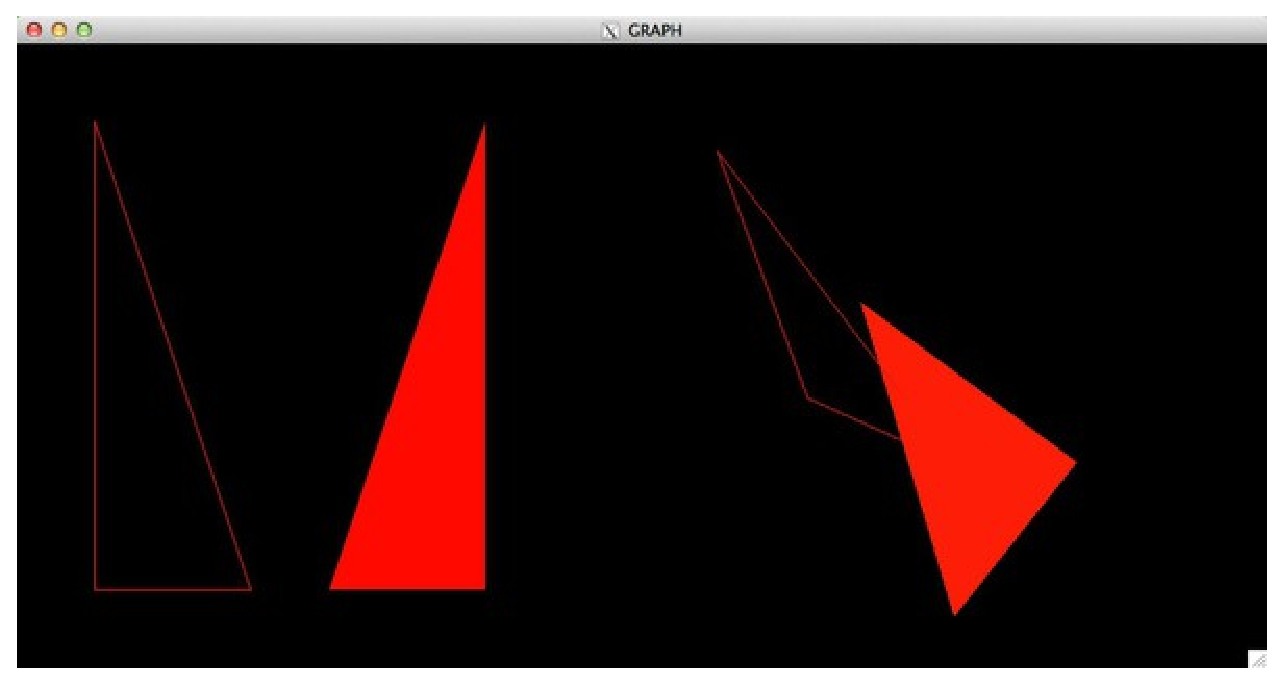
\includegraphics[width=100mm]{./Figures/eps/Canvas_g_triangle.eps}
\end{figure}
%%%%%%%%%%%%%%%%%%%%%%%%%%%%%%%%%%%%%%%%%%%%%%%%%%%%%%


%%%%%%%%%%%%%%%%%%%%%g_triangle_3D_smooth%%%%%%%%%%%%%%%%%%%%%%%%%%%%%%
\clearpage
\subsubsection{\texttt{g\_triangle\_3D\_smooth}}

\begin{itembox}[l]{\texttt{g\_triangle\_3D\_smooth}関数}
%%%%%%%%%%%%%%%%%%%ここにプロトタイプ宣言を書く%%%%%%%%%%%%%%%%%%%
\begin{verbatim}
void g_triangle_3D_smooth(
        double x0, double y0, double z0,
        double x1, double y1, double z1,
        double x2, double y2, double z2,
        double nx0, double ny0, double nz0,
        double nx1, double ny1, double nz1,
        double nx2, double ny2, double nz2,
        G_BOOL Wire, G_BOOL Fill);  
\end{verbatim}
%%%%%%%%%%%%%%%%%%%ここに引数の説明を書く%%%%%%%%%%%%%%%%%%%%%%%
\verb|x,y,z| ; 各頂点の座標\\
\verb|nx,ny,nz| ; 各頂点での法線ベクトルの$x,y,z$成分\\
%\verb|DivideLevel| ;面の三角形分割レベル($4^{\verb|DivideLevel|}$倍ずつ三角形の分割数が増える)\\
%\verb|WireFill| ; \verb|G_WIRE|:ワイヤーフレーム,\ \verb|G_FILL|:塗りつぶす \\
\verb|Wire| ; \verb|G_YES|:枠線を描く, \verb|G_NO|:枠線を描かない \\
\verb|Fill| ; \verb|G_YES|:塗りつぶす, \verb|G_NO|:塗りつぶさない 
\end{itembox}

%%%%%%%%%%%%%%%%%%%ここに関数の説明を書く%%%%%%%%%%%%%%%%%%%%%%%
\begin{itembox}[l]{\texttt{g\_triangle\_3D\_smooth}関数の説明}
三角形を描画する.(頂点の指定順によって表裏が変わることに注意.)
\end{itembox}

%%%%%%%%%%%%%%%%%%%ここに関数の説明に使う絵を載せる.%%%%%%%%%%%%%%%%
\begin{figure}[htb]
%	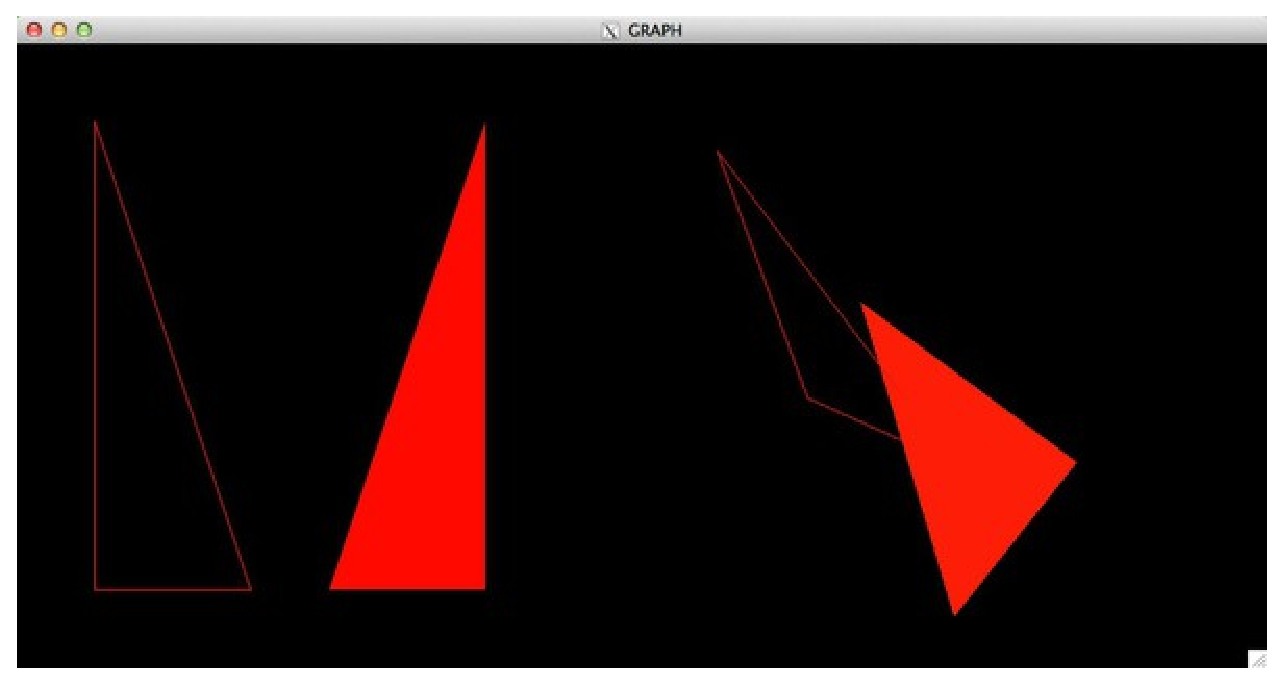
\includegraphics[width=100mm]{./Figures/eps/Canvas_g_triangle.eps}
\end{figure}
%%%%%%%%%%%%%%%%%%%%%%%%%%%%%%%%%%%%%%%%%%%%%%%%%%%%%%


%%%%%%%%%%%%%%%%%%%%%g_triangle_3D_smooth_core%%%%%%%%%%%%%%%%%%%%%%%%%%%%%%
\clearpage
\subsubsection{\texttt{g\_triangle\_3D\_smooth\_core}}

\begin{itembox}[l]{\texttt{g\_triangle\_3D\_smooth\_core}関数}
%%%%%%%%%%%%%%%%%%%ここにプロトタイプ宣言を書く%%%%%%%%%%%%%%%%%%%
\begin{verbatim}
void g_triangle_3D_smooth_smooth(
        double x0, double y0, double z0,
        double x1, double y1, double z1,
        double x2, double y2, double z2,
        double nx0, double ny0, double nz0,
        double nx1, double ny1, double nz1,
        double nx2, double ny2, double nz2,
        int DivideLevel, G_BOOL Wire, G_BOOL Fill);  
\end{verbatim}
%%%%%%%%%%%%%%%%%%%ここに引数の説明を書く%%%%%%%%%%%%%%%%%%%%%%%
\verb|x,y,z| ; 各頂点の座標\\
\verb|nx,ny,nz| ; 各頂点での法線ベクトルの$x,y,z$成分\\
\verb|DivideLevel| ;面の三角形分割レベル($4^{\verb|DivideLevel|}$倍ずつ三角形の分割数が増える)\\
%\verb|WireFill| ; \verb|G_WIRE|:ワイヤーフレーム,\ \verb|G_FILL|:塗りつぶす \\
\verb|Wire| ; \verb|G_YES|:枠線を描く, \verb|G_NO|:枠線を描かない \\
\verb|Fill| ; \verb|G_YES|:塗りつぶす, \verb|G_NO|:塗りつぶさない 
\end{itembox}

%%%%%%%%%%%%%%%%%%%ここに関数の説明を書く%%%%%%%%%%%%%%%%%%%%%%%
\begin{itembox}[l]{\texttt{g\_triangle\_3D\_smooth\_core}関数の説明}
三角形を描画する.(頂点の指定順によって表裏が変わることに注意.)
\end{itembox}

%%%%%%%%%%%%%%%%%%%ここに関数の説明に使う絵を載せる.%%%%%%%%%%%%%%%%
\begin{figure}[htb]
%	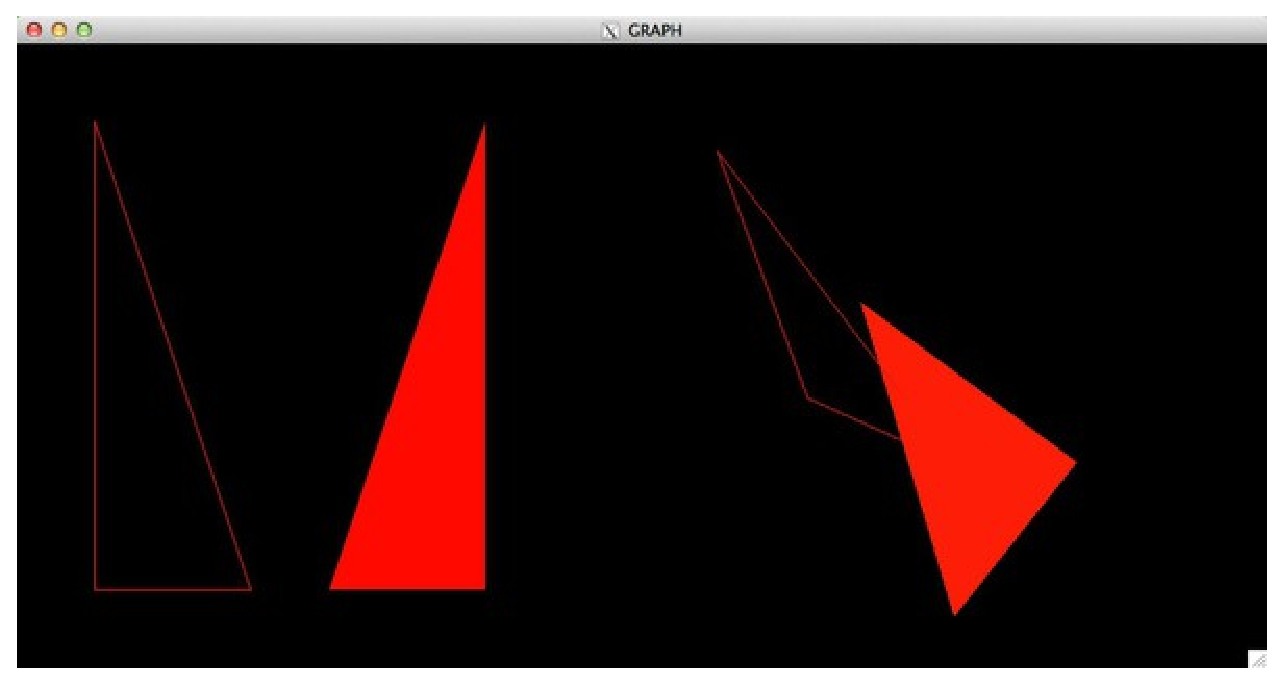
\includegraphics[width=100mm]{./Figures/eps/Canvas_g_triangle.eps}
\end{figure}
%%%%%%%%%%%%%%%%%%%%%%%%%%%%%%%%%%%%%%%%%%%%%%%%%%%%%%




%%%%%%%%%%%%%%%%%%%%%g_fan_2D%%%%%%%%%%%%%%%%%%%%%%%%%%%%%%
\clearpage
\subsubsection{\texttt{g\_fan\_2D}}

\begin{itembox}[l]{\texttt{g\_fan\_2D}関数}
%%%%%%%%%%%%%%%%%%%ここにプロトタイプ宣言を書く%%%%%%%%%%%%%%%%%%%
\begin{verbatim}
void g_fan_2D(
        double center_x, double center_y,
        double direction_x, double direction_y,
        double radius, double angle,
        G_BOOL Wire, G_BOOL Fill);
\end{verbatim}
%%%%%%%%%%%%%%%%%%%ここに引数の説明を書く%%%%%%%%%%%%%%%%%%%%%%%
\verb|center| ; 中心の座標\\
\verb|direction| ; 向き\\
\verb|radius| ; 半径\\
\verb|angle| ; 扇の中心角\\
%\verb|WireFill| ; \verb|G_WIRE|:ワイヤーフレーム,\ \verb|G_FILL|:塗りつぶす \\
\verb|Wire| ; \verb|G_YES|:枠線を描く, \verb|G_NO|:枠線を描かない \\
\verb|Fill| ; \verb|G_YES|:塗りつぶす, \verb|G_NO|:塗りつぶさない 
\end{itembox}

%%%%%%%%%%%%%%%%%%%ここに関数の説明を書く%%%%%%%%%%%%%%%%%%%%%%%
\begin{itembox}[l]{\texttt{g\_fan\_2D}関数の説明}
扇形を描画する.
\end{itembox}

%%%%%%%%%%%%%%%%%%%ここに関数の説明に使う絵を載せる.%%%%%%%%%%%%%%%%
\begin{figure}[htb]
\end{figure}
%%%%%%%%%%%%%%%%%%%%%%%%%%%%%%%%%%%%%%%%%%%%%%%%%%%%%%


%%%%%%%%%%%%%%%%%%%%%g_fan_3D%%%%%%%%%%%%%%%%%%%%%%%%%%%%%%
\clearpage
\subsubsection{\texttt{g\_fan\_3D}}

\begin{itembox}[l]{\texttt{g\_fan\_3D}関数}
%%%%%%%%%%%%%%%%%%%ここにプロトタイプ宣言を書く%%%%%%%%%%%%%%%%%%%
\begin{verbatim}
void g_fan_3D(
        double center_x, double center_y, double center_z,
        double direction_x, double direction_y, double direction_z,
        double radius, double angle, double psi,
        G_BOOL Wire, G_BOOL Fill);
\end{verbatim}
%%%%%%%%%%%%%%%%%%%ここに引数の説明を書く%%%%%%%%%%%%%%%%%%%%%%%
\verb|center| ; 中心の座標\\
\verb|direction| ; 向き\\
\verb|radius| ; 半径\\
\verb|angle| ; 扇の中心角\\
\verb|psi| ; \verb|direction|に対する回転角\\
%\verb|WireFill| ; \verb|G_WIRE|:ワイヤーフレーム,\ \verb|G_FILL|:塗りつぶす \\
\verb|Wire| ; \verb|G_YES|:枠線を描く, \verb|G_NO|:枠線を描かない \\
\verb|Fill| ; \verb|G_YES|:塗りつぶす, \verb|G_NO|:塗りつぶさない 
\end{itembox}

%%%%%%%%%%%%%%%%%%%ここに関数の説明を書く%%%%%%%%%%%%%%%%%%%%%%%
\begin{itembox}[l]{\texttt{g\_fan\_3D}関数の説明}
扇形を描画する.
\end{itembox}
\begin{figure}[htb]
\centering
	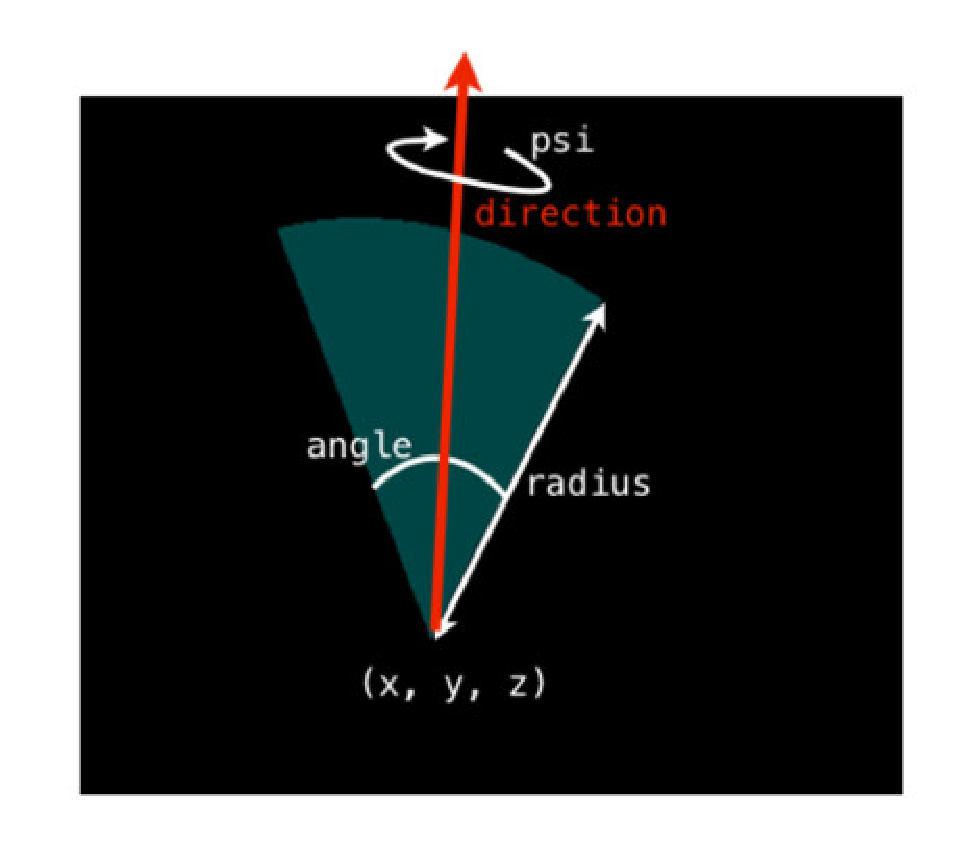
\includegraphics[width=100mm]{./Figures/eps/Canvas_g_fan.eps}
\end{figure}

%%%%%%%%%%%%%%%%%%%ここに関数の説明に使う絵を載せる.%%%%%%%%%%%%%%%%
%%%%%%%%%%%%%%%%%%%%%%%%%%%%%%%%%%%%%%%%%%%%%%%%%%%%%%


%%%%%%%%%%%%%%%%%%%%%g_fan_3D_core%%%%%%%%%%%%%%%%%%%%%%%%%%%%%%
\clearpage
\subsubsection{\texttt{g\_fan\_3D\_core}}

\begin{itembox}[l]{\texttt{g\_fan\_3D\_core}関数}
%%%%%%%%%%%%%%%%%%%ここにプロトタイプ宣言を書く%%%%%%%%%%%%%%%%%%%
\begin{verbatim}
void g_fan_3D_core(
        double center_x, double center_y, double center_z,
        double direction_x, double direction_y, double direction_z,
        double radius, double angle, double psi,
        int FaceNumberLevel, int DivideLevel, G_BOOL Wire, G_BOOL Fill);
\end{verbatim}
%%%%%%%%%%%%%%%%%%%ここに引数の説明を書く%%%%%%%%%%%%%%%%%%%%%%%
\verb|center| ; 中心の座標\\
\verb|direction| ; 向き\\
\verb|radius| ; 半径\\
\verb|angle| ; 扇の中心角\\
\verb|psi| ; \verb|direction|に対する回転角\\
\verb|FaceNumberLevel| ; 扇形の分割レベル\\
\verb|DivideLevel| ;面の三角形分割レベル($4^{\verb|DivideLevel|}$倍ずつ三角形の分割数が増える)\\
%\verb|WireFill| ; \verb|G_WIRE|:ワイヤーフレーム,\ \verb|G_FILL|:塗りつぶす \\
\verb|Wire| ; \verb|G_YES|:枠線を描く, \verb|G_NO|:枠線を描かない \\
\verb|Fill| ; \verb|G_YES|:塗りつぶす, \verb|G_NO|:塗りつぶさない 
\end{itembox}

%%%%%%%%%%%%%%%%%%%ここに関数の説明を書く%%%%%%%%%%%%%%%%%%%%%%%
\begin{itembox}[l]{\texttt{g\_fan\_3D\_core}関数の説明}
扇形を描画する.(より細かい設定が可能)
\end{itembox}
\begin{figure}[htb]
\centering
	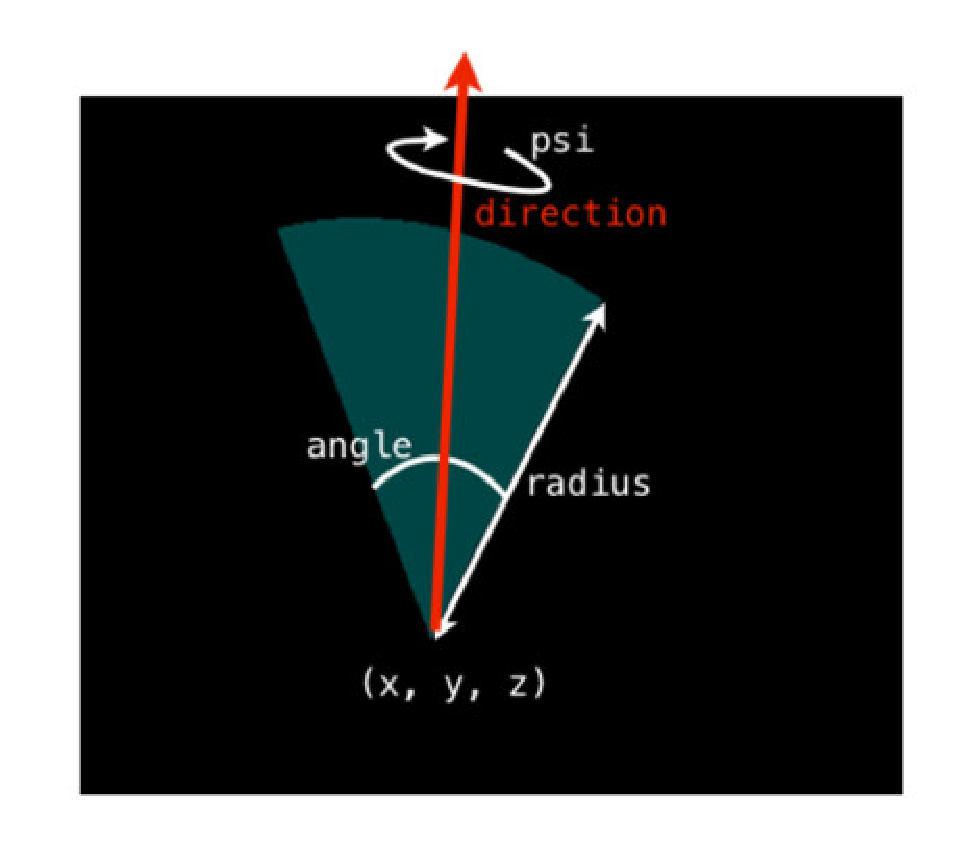
\includegraphics[width=100mm]{./Figures/eps/Canvas_g_fan.eps}
\end{figure}

%%%%%%%%%%%%%%%%%%%ここに関数の説明に使う絵を載せる.%%%%%%%%%%%%%%%%
\begin{figure}[htb]
\centering
	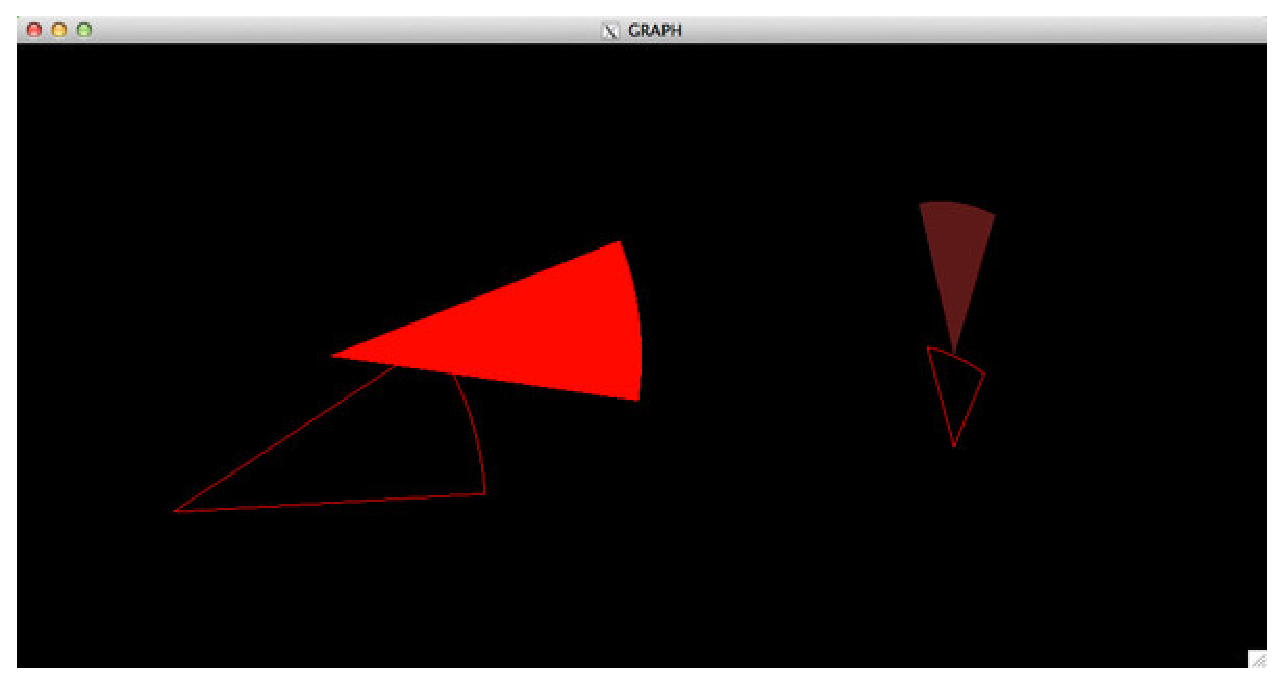
\includegraphics[width=100mm]{./Figures/eps/Canvas_g_fan2.eps}
\end{figure}
%%%%%%%%%%%%%%%%%%%%%%%%%%%%%%%%%%%%%%%%%%%%%%%%%%%%%%




%%%%%%%%%%%%%%%%%%%%%g_circle_2D%%%%%%%%%%%%%%%%%%%%%%%%%%%%%%
\clearpage
\subsubsection{\texttt{g\_circle\_2D}}

\begin{itembox}[l]{\texttt{g\_circle\_2D}関数}
%%%%%%%%%%%%%%%%%%%ここにプロトタイプ宣言を書く%%%%%%%%%%%%%%%%%%%
\begin{verbatim}
void g_circle_2D(
        double center_x, double center_y,
        double radius, G_BOOL Wire, G_BOOL Fill);
\end{verbatim}
%%%%%%%%%%%%%%%%%%%ここに引数の説明を書く%%%%%%%%%%%%%%%%%%%%%%%
\verb|center| ; 中心の座標\\
\verb|radius| ; 半径\\
%\verb|WireFill| ; \verb|G_WIRE|:ワイヤーフレーム,\ \verb|G_FILL|:塗りつぶす \\
\verb|Wire| ; \verb|G_YES|:枠線を描く, \verb|G_NO|:枠線を描かない \\
\verb|Fill| ; \verb|G_YES|:塗りつぶす, \verb|G_NO|:塗りつぶさない 
\end{itembox}

%%%%%%%%%%%%%%%%%%%ここに関数の説明を書く%%%%%%%%%%%%%%%%%%%%%%%
\begin{itembox}[l]{\texttt{g\_circle\_2D}関数の説明}
円を描画する.
\end{itembox}

%%%%%%%%%%%%%%%%%%%ここに関数の説明に使う絵を載せる.%%%%%%%%%%%%%%%%
\begin{figure}[htb]
\end{figure}
%%%%%%%%%%%%%%%%%%%%%%%%%%%%%%%%%%%%%%%%%%%%%%%%%%%%%%


%%%%%%%%%%%%%%%%%%%%%g_circle_3D%%%%%%%%%%%%%%%%%%%%%%%%%%%%%%
\clearpage
\subsubsection{\texttt{g\_circle\_3D}}

\begin{itembox}[l]{\texttt{g\_circle\_3D}関数}
%%%%%%%%%%%%%%%%%%%ここにプロトタイプ宣言を書く%%%%%%%%%%%%%%%%%%%
\begin{verbatim}
void g_circle_3D(
        double center_x, double center_y,
        double radius, double theta, double phi, 
        G_BOOL Wire, G_BOOL Fill);
\end{verbatim}
%%%%%%%%%%%%%%%%%%%ここに引数の説明を書く%%%%%%%%%%%%%%%%%%%%%%%
\verb|center| ; 中心の座標\\
\verb|radius| ; 半径\\
\verb|psi| ; 半径\\
\verb|theta| ; 半径\\
\verb|Wire| ; \verb|G_YES|:枠線を描く, \verb|G_NO|:枠線を描かない \\
\verb|Fill| ; \verb|G_YES|:塗りつぶす, \verb|G_NO|:塗りつぶさない 
\end{itembox}

%%%%%%%%%%%%%%%%%%%ここに関数の説明を書く%%%%%%%%%%%%%%%%%%%%%%%
\begin{itembox}[l]{\texttt{g\_circle\_3D}関数の説明}
円板を描画する.
\end{itembox}

%%%%%%%%%%%%%%%%%%%ここに関数の説明に使う絵を載せる.%%%%%%%%%%%%%%%%
%%%%%%%%%%%%%%%%%%%%%%%%%%%%%%%%%%%%%%%%%%%%%%%%%%%%%%





%%%%%%%%%%%%%%%%%%%%%g_circle_3D_core%%%%%%%%%%%%%%%%%%%%%%%%%%%%%%
\clearpage
\subsubsection{\texttt{g\_circle\_3D\_core}}

\begin{itembox}[l]{\texttt{g\_circle\_3D\_core}関数}
%%%%%%%%%%%%%%%%%%%ここにプロトタイプ宣言を書く%%%%%%%%%%%%%%%%%%%
\begin{verbatim}
void g_circle_3D_core(
        double center_x, double center_y,
        double radius, double theta, double phi,        
        int N, int DivideLevel, G_BOOL Wire, G_BOOL Fill);
\end{verbatim}
%%%%%%%%%%%%%%%%%%%ここに引数の説明を書く%%%%%%%%%%%%%%%%%%%%%%%
\verb|center| ; 中心の座標\\
\verb|radius| ; 半径\\
\verb|psi| ; 半径\\
\verb|theta| ; 半径\\
\verb|N| ; 円周の分割数 \\
\verb|DivideLevel| ; 面の三角形分割レベル($4^{\verb|DivideLevel|}$倍ずつ三角形の分割数が増える)\\
%\verb|WireFill| ; \verb|G_WIRE|:ワイヤーフレーム,\ \verb|G_FILL|:塗りつぶす \\
\verb|Wire| ; \verb|G_YES|:枠線を描く, \verb|G_NO|:枠線を描かない \\
\verb|Fill| ; \verb|G_YES|:塗りつぶす, \verb|G_NO|:塗りつぶさない 
\end{itembox}

%%%%%%%%%%%%%%%%%%%ここに関数の説明を書く%%%%%%%%%%%%%%%%%%%%%%%
\begin{itembox}[l]{\texttt{g\_circle\_3D\_core}関数の説明}
円板を描画する.(より細かい設定が可能)
\end{itembox}
\begin{figure}[htb]
\centering
	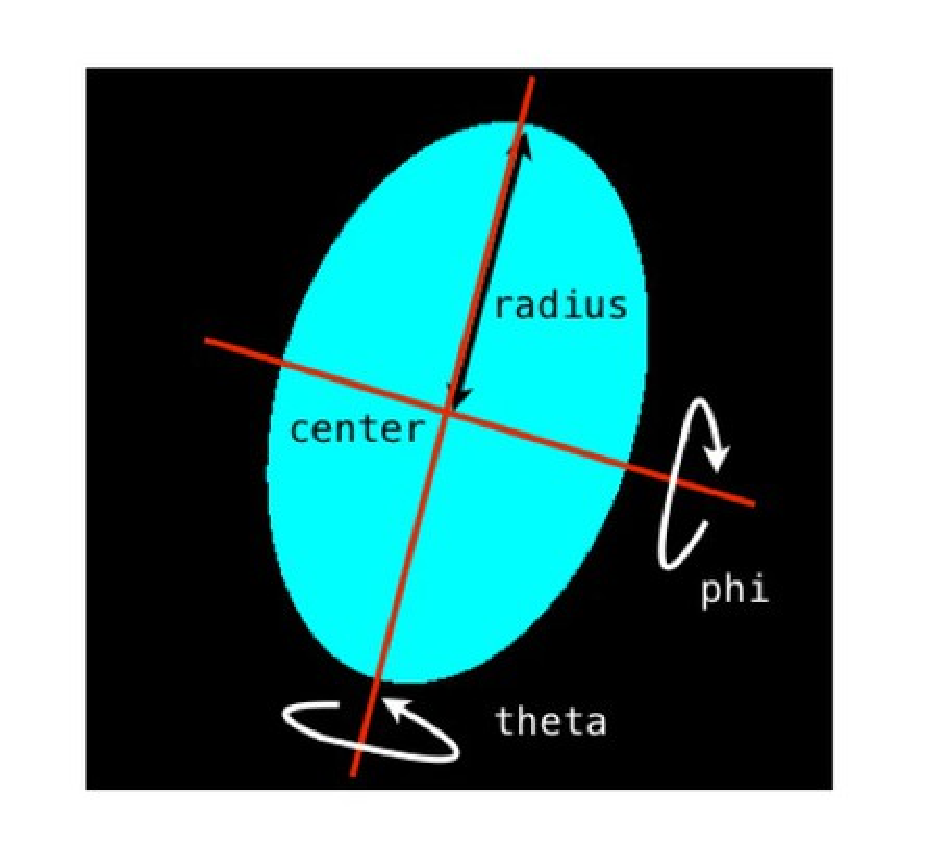
\includegraphics[width=100mm]{./Figures/eps/Canvas_g_circle.eps}
\end{figure}

%%%%%%%%%%%%%%%%%%%ここに関数の説明に使う絵を載せる.%%%%%%%%%%%%%%%%
\begin{figure}[htb]
\centering
	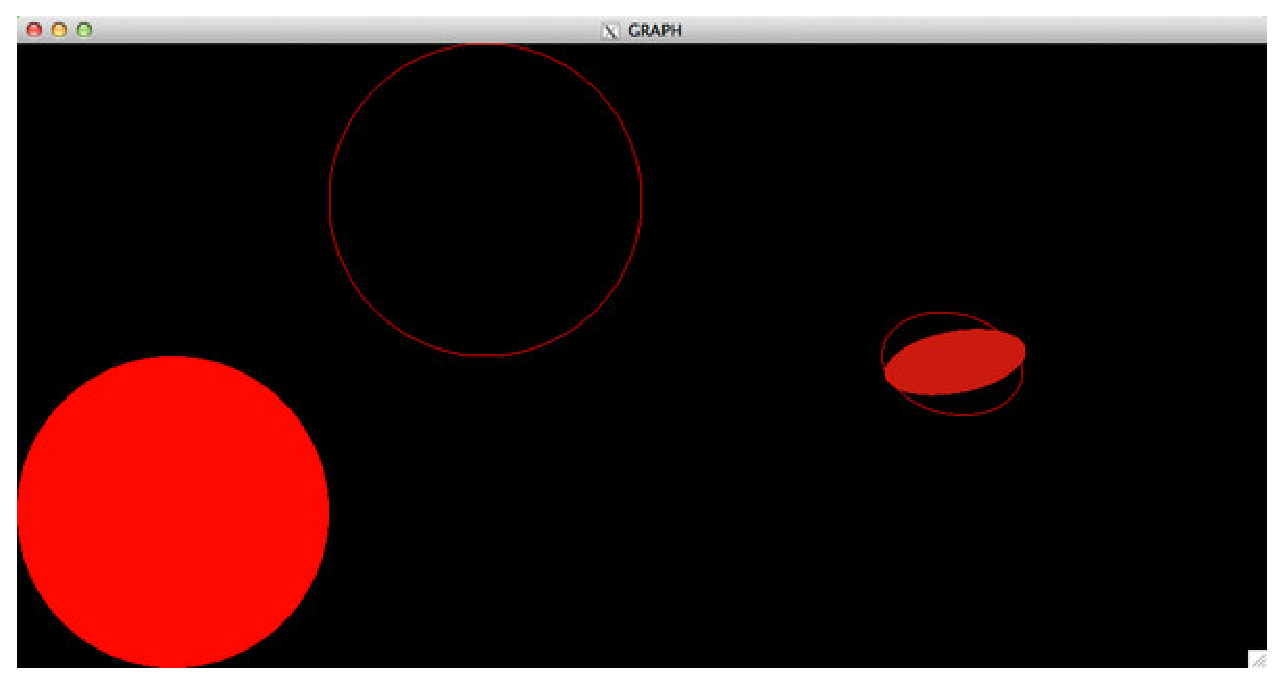
\includegraphics[width=100mm]{./Figures/eps/Canvas_g_circle2.eps}
\end{figure}
%%%%%%%%%%%%%%%%%%%%%%%%%%%%%%%%%%%%%%%%%%%%%%%%%%%%%%




%%%%%%%%%%%%%%%%%%%%%g_polygon_2D%%%%%%%%%%%%%%%%%%%%%%%%%%%%%%
\clearpage
\subsubsection{\texttt{g\_polygon\_2D}}

\begin{itembox}[l]{\texttt{g\_polygon\_2D}関数}
%%%%%%%%%%%%%%%%%%%ここにプロトタイプ宣言を書く%%%%%%%%%%%%%%%%%%%
\begin{verbatim}
void g_polygon_2D(
        double *xx, double *yy,
        int n, G_BOOL WIRE, G_BOOL FILL);
\end{verbatim}
%%%%%%%%%%%%%%%%%%%ここに引数の説明を書く%%%%%%%%%%%%%%%%%%%%%%%
\verb|xx,yy| ; 頂点データを格納した一次元配列\\
\verb|n| ; 配列の数\\
%\verb|WireFill| ; \verb|G_WIRE|:ワイヤーフレーム,\ \verb|G_FILL|:塗りつぶす \\
\verb|Wire| ; \verb|G_YES|:枠線を描く, \verb|G_NO|:枠線を描かない \\
\verb|Fill| ; \verb|G_YES|:塗りつぶす, \verb|G_NO|:塗りつぶさない 
\end{itembox}

%%%%%%%%%%%%%%%%%%%ここに関数の説明を書く%%%%%%%%%%%%%%%%%%%%%%%
\begin{itembox}[l]{\texttt{g\_polygon\_2D}関数の説明}
多角形を描画する.
\end{itembox}

%%%%%%%%%%%%%%%%%%%ここに関数の説明に使う絵を載せる.%%%%%%%%%%%%%%%%
\begin{figure}[htb]
\centering
	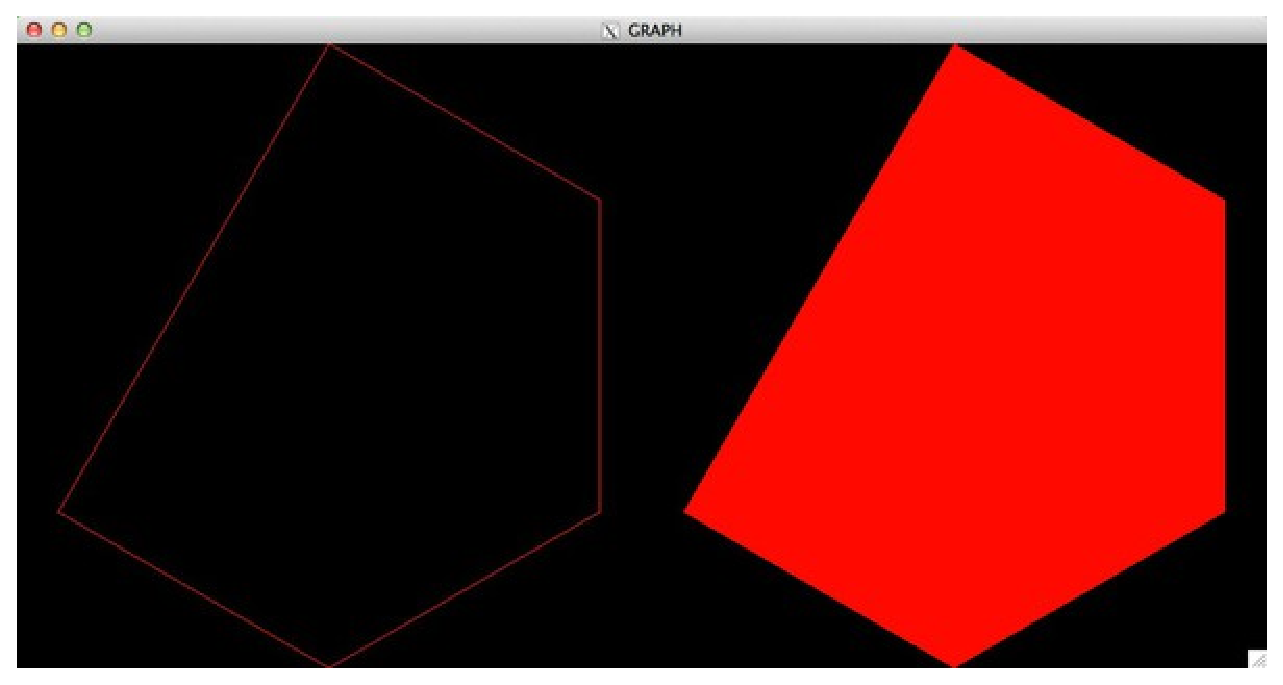
\includegraphics[width=100mm]{./Figures/eps/Canvas_g_polygon.eps}
\end{figure}
%%%%%%%%%%%%%%%%%%%%%%%%%%%%%%%%%%%%%%%%%%%%%%%%%%%%%%




%%%%%%%%%%%%%%%%%%%%%g_polyline_2D%%%%%%%%%%%%%%%%%%%%%%%%%%%%%%
\clearpage
\subsubsection{\texttt{g\_polyline\_2D}}

\begin{itembox}[l]{\texttt{g\_polyline\_2D}関数}
%%%%%%%%%%%%%%%%%%%ここにプロトタイプ宣言を書く%%%%%%%%%%%%%%%%%%%
\begin{verbatim}
void g_polyline_2D(
        double *xx, double *yy,
        int n);
\end{verbatim}
%%%%%%%%%%%%%%%%%%%ここに引数の説明を書く%%%%%%%%%%%%%%%%%%%%%%%
\verb|xx,yy| ; 頂点データを格納した一次元配列\\
\verb|n| ; 配列の数
\end{itembox}

%%%%%%%%%%%%%%%%%%%ここに関数の説明を書く%%%%%%%%%%%%%%%%%%%%%%%
\begin{itembox}[l]{\texttt{g\_polyline\_2D}関数の説明}
与えられた点列を線分で連続的に結んだものを描画する.
\end{itembox}

%%%%%%%%%%%%%%%%%%%ここに関数の説明に使う絵を載せる.%%%%%%%%%%%%%%%%
%%%%%%%%%%%%%%%%%%%%%%%%%%%%%%%%%%%%%%%%%%%%%%%%%%%%%%



%%%%%%%%%%%%%%%%%%%%%g_polyline_3D%%%%%%%%%%%%%%%%%%%%%%%%%%%%%%
\clearpage
\subsubsection{\texttt{g\_polyline\_3D}}

\begin{itembox}[l]{\texttt{g\_polyline\_3D}関数}
%%%%%%%%%%%%%%%%%%%ここにプロトタイプ宣言を書く%%%%%%%%%%%%%%%%%%%
\begin{verbatim}
void g_polyline_3D(
        double *xx, double *yy, double *zz,
        int n);
\end{verbatim}
%%%%%%%%%%%%%%%%%%%ここに引数の説明を書く%%%%%%%%%%%%%%%%%%%%%%%
\verb|xx,yy,zz| ; 頂点データを格納した一次元配列\\
\verb|n| ; 配列の数
\end{itembox}

%%%%%%%%%%%%%%%%%%%ここに関数の説明を書く%%%%%%%%%%%%%%%%%%%%%%%
\begin{itembox}[l]{\texttt{g\_polyline\_3D}関数の説明}
与えられた点列を線分で連続的に結んだものを描画する.
\end{itembox}

%%%%%%%%%%%%%%%%%%%ここに関数の説明に使う絵を載せる.%%%%%%%%%%%%%%%%
\begin{figure}[htb]
\centering
	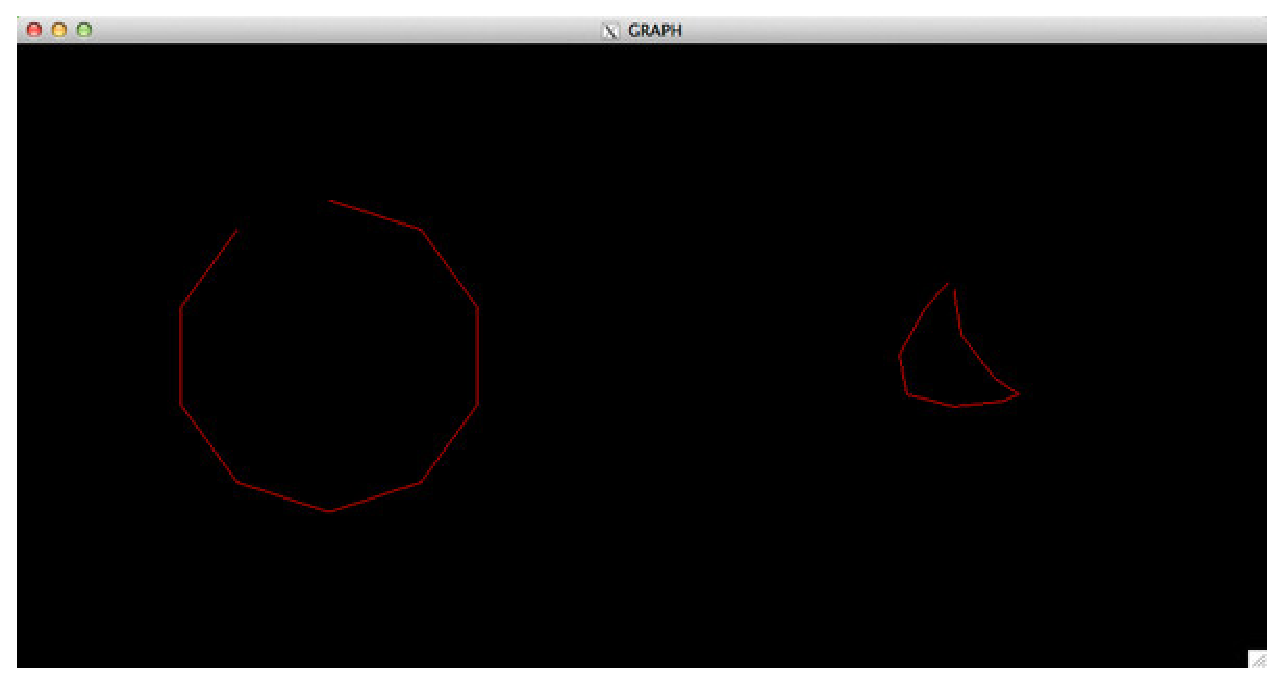
\includegraphics[width=100mm]{./Figures/eps/Canvas_g_polyline.eps}
\end{figure}
%%%%%%%%%%%%%%%%%%%%%%%%%%%%%%%%%%%%%%%%%%%%%%%%%%%%%%



%%%%%%%%%%%%%%%%%%%%%g_rectangle_3D%%%%%%%%%%%%%%%%%%%%%%%%%%%%%%
\clearpage
\subsubsection{\texttt{g\_rectangle\_3D}}

\begin{itembox}[l]{\texttt{g\_rectangle\_3D}関数}
%%%%%%%%%%%%%%%%%%%ここにプロトタイプ宣言を書く%%%%%%%%%%%%%%%%%%%
\begin{verbatim}
void g_rectangle_3D(
        double center_x, double center_y, double center_z,
        double direction_x, double direction_y, double direction_z,
        double width, double depth, double psi,
        G_BOOL WIRE, G_BOOL FILL);
\end{verbatim}
%%%%%%%%%%%%%%%%%%%ここに引数の説明を書く%%%%%%%%%%%%%%%%%%%%%%%
\verb|center| ; 重心の座標\\
\verb|direction| ; 向き\\
\verb|width,height,depth| ; 幅,高さ,奥行き\\
\verb|psi| ; \verb|direction|に対する回転角\\
\verb|Wire| ; \verb|G_YES|:枠線を描く, \verb|G_NO|:枠線を描かない \\
\verb|Fill| ; \verb|G_YES|:塗りつぶす, \verb|G_NO|:塗りつぶさない 
\end{itembox}

%%%%%%%%%%%%%%%%%%%ここに関数の説明を書く%%%%%%%%%%%%%%%%%%%%%%%
\begin{itembox}[l]{\texttt{g\_rectangle\_3D}関数の説明}
長方形を描画する.
\end{itembox}

%%%%%%%%%%%%%%%%%%%ここに関数の説明に使う絵を載せる.%%%%%%%%%%%%%%%%
%%%%%%%%%%%%%%%%%%%%%%%%%%%%%%%%%%%%%%%%%%%%%%%%%%%%%%


%%%%%%%%%%%%%%%%%%%%%g_rectangle_3D_core%%%%%%%%%%%%%%%%%%%%%%%%%%%%%%
\clearpage
\subsubsection{\texttt{g\_rectangle\_3D\_core}}

\begin{itembox}[l]{\texttt{g\_rectangle\_3D\_core}関数}
%%%%%%%%%%%%%%%%%%%ここにプロトタイプ宣言を書く%%%%%%%%%%%%%%%%%%%
\begin{verbatim}
void g_rectangle_3D_core(
        double center_x, double center_y, double center_z,
        double direction_x, double direction_y, double direction_z,
        double width, double depth, double psi,
        int DivideLevel, G_BOOL WIRE, G_BOOL FILL);
\end{verbatim}
%%%%%%%%%%%%%%%%%%%ここに引数の説明を書く%%%%%%%%%%%%%%%%%%%%%%%
\verb|center| ; 重心の座標\\
\verb|direction| ; 向き\\
\verb|width,height,depth| ; 幅,高さ,奥行き\\
\verb|psi| ; \verb|direction|に対する回転角\\
\verb|DivideLevel| ;面の三角形分割レベル($4^{\verb|DivideLevel|}$倍ずつ三角形の分割数が増える)\\
%\verb|WireFill| ; \verb|G_WIRE|:ワイヤーフレーム,\ \verb|G_FILL|:塗りつぶす \\
\verb|Wire| ; \verb|G_YES|:枠線を描く, \verb|G_NO|:枠線を描かない \\
\verb|Fill| ; \verb|G_YES|:塗りつぶす, \verb|G_NO|:塗りつぶさない 
\end{itembox}

%%%%%%%%%%%%%%%%%%%ここに関数の説明を書く%%%%%%%%%%%%%%%%%%%%%%%
\begin{itembox}[l]{\texttt{g\_rectangle\_3D\_core}関数の説明}
長方形を描画する.
(より細かい設定が可能.)
\end{itembox}

%%%%%%%%%%%%%%%%%%%ここに関数の説明に使う絵を載せる.%%%%%%%%%%%%%%%%
\begin{figure}[htb]
\centering
	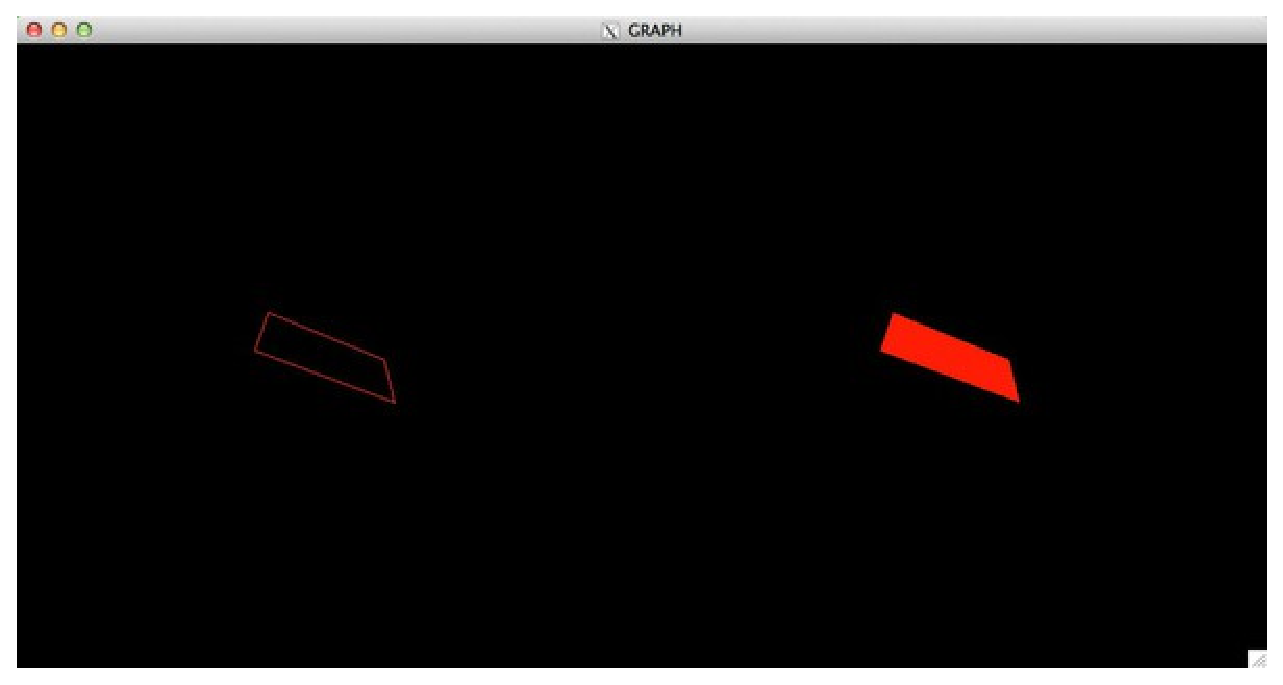
\includegraphics[width=100mm]{./Figures/eps/Canvas_g_rectangle.eps}
\end{figure}
%%%%%%%%%%%%%%%%%%%%%%%%%%%%%%%%%%%%%%%%%%%%%%%%%%%%%%




%%%%%%%%%%%%%%%%%%%%%g_data_plot_2D%%%%%%%%%%%%%%%%%%%%%%%%%%%%%%
\clearpage
\subsubsection{\texttt{g\_data\_plot\_2D}}

\begin{itembox}[l]{\texttt{g\_data\_plot\_2D}関数}
%%%%%%%%%%%%%%%%%%%ここにプロトタイプ宣言を書く%%%%%%%%%%%%%%%%%%%
\begin{verbatim}
void g_data_plot_2D(
        double x0, double x1,
        double y0, double y1,
        int number_x,
        double u[number_x]);
\end{verbatim}
%%%%%%%%%%%%%%%%%%%ここに引数の説明を書く%%%%%%%%%%%%%%%%%%%%%%%
\verb|x,y| ; 描画範囲の指定\\
\verb|number| ; 配列\verb|u|のサイズ\\
\verb|u| ; データの格納された1次元配列
\end{itembox}

%%%%%%%%%%%%%%%%%%%ここに関数の説明を書く%%%%%%%%%%%%%%%%%%%%%%%
\begin{itembox}[l]{\texttt{g\_data\_plot\_2D}関数の説明}
1次元配列\verb|u|のデータをプロットする.
\end{itembox}

%%%%%%%%%%%%%%%%%%%ここに関数の説明に使う絵を載せる.%%%%%%%%%%%%%%%%
%%%%%%%%%%%%%%%%%%%%%%%%%%%%%%%%%%%%%%%%%%%%%%%%%%%%%%


%%%%%%%%%%%%%%%%%%%%%g_data_plot_3D%%%%%%%%%%%%%%%%%%%%%%%%%%%%%%
\clearpage
\subsubsection{\texttt{g\_data\_plot\_3D}}

\begin{itembox}[l]{\texttt{g\_data\_plot\_3D}関数}
%%%%%%%%%%%%%%%%%%%ここにプロトタイプ宣言を書く%%%%%%%%%%%%%%%%%%%
\begin{verbatim}
void g_data_plot_3D(
        double x0, double x1,
        double y0, double y1,
        double z0, double z1,
        int number_x, int number_y,
        double u[number_x][number_y]);
\end{verbatim}
%%%%%%%%%%%%%%%%%%%ここに引数の説明を書く%%%%%%%%%%%%%%%%%%%%%%%
\verb|x,y,z| ; 描画範囲の指定\\
\verb|number| ; 配列\verb|u|の各方向のサイズ\\
\verb|u| ; 2次元配列もしくは1次元配列を2次元配列化*した配列
\end{itembox}

%%%%%%%%%%%%%%%%%%%ここに関数の説明を書く%%%%%%%%%%%%%%%%%%%%%%%
\begin{itembox}[l]{\texttt{g\_data\_plot\_3D}関数の説明}
2次元配列\verb|u|のデータをプロットする.(2次元配列化*に関しては前章をお読みください.c++では使用不可であることに注意.)
\end{itembox}

%%%%%%%%%%%%%%%%%%%ここに関数の説明に使う絵を載せる.%%%%%%%%%%%%%%%%
\begin{figure}[htb]
\end{figure}
%%%%%%%%%%%%%%%%%%%%%%%%%%%%%%%%%%%%%%%%%%%%%%%%%%%%%%




%%%%%%%%%%%%%%%%%%%%%g_data_plot_f_3D%%%%%%%%%%%%%%%%%%%%%%%%%%%%%%
\clearpage
\subsubsection{\texttt{g\_data\_plot\_f\_3D}}

\begin{itembox}[l]{\texttt{g\_data\_plot\_f\_3D}関数}
%%%%%%%%%%%%%%%%%%%ここにプロトタイプ宣言を書く%%%%%%%%%%%%%%%%%%%
\begin{verbatim}
void g_data_plot_f_3D(
        double x0, double x1,
        double y0, double y1,
        double z0, double z1,
        int number_x, int number_y,
        double *u);
\end{verbatim}
%%%%%%%%%%%%%%%%%%%ここに引数の説明を書く%%%%%%%%%%%%%%%%%%%%%%%
\verb|x,y,z| ; 描画範囲の指定\\
\verb|number| ; 配列\verb|u|の各方向のサイズ\\
\verb|u| ; 1次元配列を2次元配列化*した配列
\end{itembox}

%%%%%%%%%%%%%%%%%%%ここに関数の説明を書く%%%%%%%%%%%%%%%%%%%%%%%
\begin{itembox}[l]{\texttt{g\_data\_plot\_f\_3D}関数の説明}
1次元配列\verb|u|のデータをプロットする.(2次元配列化*に関しては前章をお読みください.)
\end{itembox}

%%%%%%%%%%%%%%%%%%%ここに関数の説明に使う絵を載せる.%%%%%%%%%%%%%%%%
\begin{figure}[htb]
\centering
	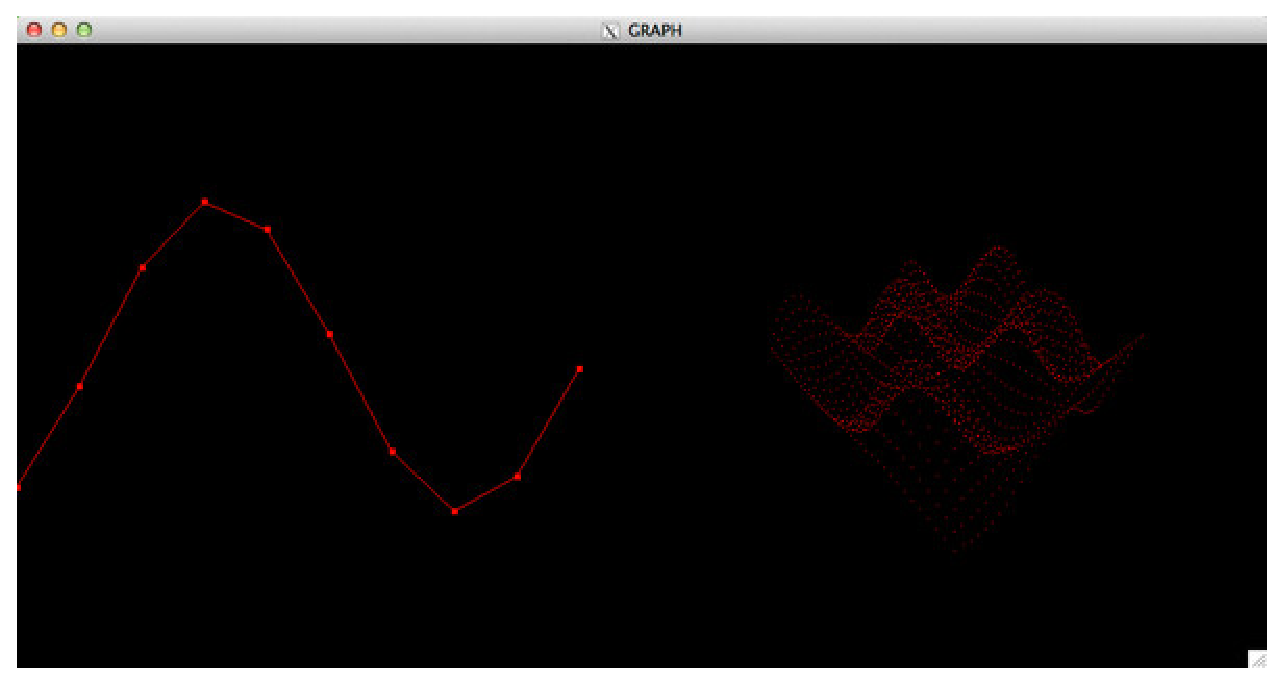
\includegraphics[width=100mm]{./Figures/eps/Canvas_g_data_plot.eps}
\end{figure}
%%%%%%%%%%%%%%%%%%%%%%%%%%%%%%%%%%%%%%%%%%%%%%%%%%%%%%




\clearpage
\subsection{上位関数}
%%%%%%%%%%%%%%%%%%%%%g_contln_2D%%%%%%%%%%%%%%%%%%%%%%%%%%%%%%
\subsubsection{\texttt{g\_contln\_2D}}

\begin{itembox}[l]{\texttt{g\_contln\_2D}関数}
%%%%%%%%%%%%%%%%%%%ここにプロトタイプ宣言を書く%%%%%%%%%%%%%%%%%%%
\begin{verbatim}
void g_contln_2D(
        double x_left, double x_right,
        double y_bottom, double y_top,
        int N_x, int N_y,
        double data2D[N_x][N_y],
        double level);
\end{verbatim}
%%%%%%%%%%%%%%%%%%%ここに引数の説明を書く%%%%%%%%%%%%%%%%%%%%%%%
\verb|x,y| ; 描画範囲の指定\\
\verb|N| ; 配列\verb|u|の各方向のサイズ\\
\verb|data2D| ; データの格納された2次元配列もしくは1次元配列を2次元配列化*した配列\\
\verb|level| ; 等高線を引きたい値.
\end{itembox}

%%%%%%%%%%%%%%%%%%%ここに関数の説明を書く%%%%%%%%%%%%%%%%%%%%%%%
\begin{itembox}[l]{\texttt{g\_contln\_2D}関数の説明}
2次元配列\verb|u|に対して,値\verb|level|に等高線を描画する.
(2次元配列化*に関しては前章をお読みください.c++では使用不可であることに注意.)
\end{itembox}

%%%%%%%%%%%%%%%%%%%ここに関数の説明に使う絵を載せる.%%%%%%%%%%%%%%%%
\begin{figure}[htb]
\end{figure}
%%%%%%%%%%%%%%%%%%%%%%%%%%%%%%%%%%%%%%%%%%%%%%%%%%%%%%




%%%%%%%%%%%%%%%%%%%%%g_contln_f_2D%%%%%%%%%%%%%%%%%%%%%%%%%%%%%%
\clearpage
\subsubsection{\texttt{g\_contln\_f\_2D}}

\begin{itembox}[l]{\texttt{g\_contln\_f\_2D}関数}
%%%%%%%%%%%%%%%%%%%ここにプロトタイプ宣言を書く%%%%%%%%%%%%%%%%%%%
\begin{verbatim}
void g_contln_f_2D(
        double x_left, double x_right,
        double y_bottom, double y_top,
        int N_x, int N_y,
        double *data2D,
        double level);
\end{verbatim}
%%%%%%%%%%%%%%%%%%%ここに引数の説明を書く%%%%%%%%%%%%%%%%%%%%%%%
\verb|x,y| ; 描画範囲の指定\\
\verb|N| ; 配列\verb|u|の各方向のサイズ\\
\verb|data2D| ; データの格納された,1次元配列を2次元配列化*した配列\\
\verb|level| ; 等高線を引きたい値.
\end{itembox}

%%%%%%%%%%%%%%%%%%%ここに関数の説明を書く%%%%%%%%%%%%%%%%%%%%%%%
\begin{itembox}[l]{\texttt{g\_contln\_f\_2D}関数の説明}
1次元配列\verb|u|に対して,値\verb|level|に等高線を描画する.
(2次元配列化*に関しては前章をお読みください.)
\end{itembox}

%%%%%%%%%%%%%%%%%%%ここに関数の説明に使う絵を載せる.%%%%%%%%%%%%%%%%
\begin{figure}[htb]
\centering
	\includegraphics[width=100mm]{./Figures/eps/Canvas_g_contln.eps}
\end{figure}
%%%%%%%%%%%%%%%%%%%%%%%%%%%%%%%%%%%%%%%%%%%%%%%%%%%%%%




%%%%%%%%%%%%%%%%%%%%%g_bird_view_3D%%%%%%%%%%%%%%%%%%%%%%%%%%%%%%
\clearpage
\subsubsection{\texttt{g\_bird\_view\_3D}}

\begin{itembox}[l]{\texttt{g\_bird\_view\_3D}関数}
%%%%%%%%%%%%%%%%%%%ここにプロトタイプ宣言を書く%%%%%%%%%%%%%%%%%%%
\begin{verbatim}
void g_bird_view_3D(
        double x_left, double x_right, 
        double y_bottom, double y_top,
        int number_x, int number_y,
        double u[number_x][number_y],
        G_BOOL WIRE, G_BOOL FILL);
\end{verbatim}
%%%%%%%%%%%%%%%%%%%ここに引数の説明を書く%%%%%%%%%%%%%%%%%%%%%%%
\verb|x,y,z| ; 描画範囲の指定\\
\verb|number| ; 配列\verb|u|の各方向のサイズ\\
\verb|u| ; 2次元配列もしくは1次元配列を2次元配列化*した配列\\
%\verb|WireFill| ; \verb|G_WIRE|:ワイヤーフレーム,\ \verb|G_FILL|:塗りつぶす \\
\verb|Wire| ; \verb|G_YES|:枠線を描く, \verb|G_NO|:枠線を描かない \\
\verb|Fill| ; \verb|G_YES|:塗りつぶす, \verb|G_NO|:塗りつぶさない 
\end{itembox}

%%%%%%%%%%%%%%%%%%%ここに関数の説明を書く%%%%%%%%%%%%%%%%%%%%%%%
\begin{itembox}[l]{\texttt{g\_bird\_view\_3D}関数の説明}
2次元配列\verb|u|に対して鳥瞰図を描画する.\verb|y_top|$=$\verb|y_bottom|とするとy方向のスケーリングをせず,値をそのまま反映する.
(2次元配列化*に関しては前章をお読みください.c++では使用不可であることに注意.)
\end{itembox}

%%%%%%%%%%%%%%%%%%%ここに関数の説明に使う絵を載せる.%%%%%%%%%%%%%%%%
%%%%%%%%%%%%%%%%%%%%%%%%%%%%%%%%%%%%%%%%%%%%%%%%%%%%%%




%%%%%%%%%%%%%%%%%%%%%g_bird_view_f_3D%%%%%%%%%%%%%%%%%%%%%%%%%%%%%%
\clearpage
\subsubsection{\texttt{g\_bird\_view\_f\_3D}}

\begin{itembox}[l]{\texttt{g\_bird\_view\_f\_3D}関数}
%%%%%%%%%%%%%%%%%%%ここにプロトタイプ宣言を書く%%%%%%%%%%%%%%%%%%%
\begin{verbatim}
void g_bird_view_f_3D(
        double x_left, double x_right, 
        double y_bottom, double y_top,
        int number_x, int number_y,
        double *u, G_BOOL WIRE, G_BOOL FILL);
\end{verbatim}
%%%%%%%%%%%%%%%%%%%ここに引数の説明を書く%%%%%%%%%%%%%%%%%%%%%%%
\verb|x,y,z| ; 描画範囲の指定\\
\verb|number| ; 配列\verb|u|の各方向のサイズ\\
\verb|u| ;1次元配列を2次元配列化*した配列\\
%\verb|WireFill| ; \verb|G_WIRE|:ワイヤーフレーム,\ \verb|G_FILL|:塗りつぶす \\
\verb|Wire| ; \verb|G_YES|:枠線を描く, \verb|G_NO|:枠線を描かない \\
\verb|Fill| ; \verb|G_YES|:塗りつぶす, \verb|G_NO|:塗りつぶさない 
\end{itembox}

%%%%%%%%%%%%%%%%%%%ここに関数の説明を書く%%%%%%%%%%%%%%%%%%%%%%%
\begin{itembox}[l]{\texttt{g\_bird\_view\_f\_3D}関数の説明}
1次元配列\verb|u|に対して鳥瞰図を描画する.\verb|y_top|$=$\verb|y_bottom|とするとy方向のスケーリングをせず,値をそのまま反映する.
(2次元配列化*に関しては前章をお読みください.)
\end{itembox}

%%%%%%%%%%%%%%%%%%%ここに関数の説明に使う絵を載せる.%%%%%%%%%%%%%%%%
\begin{figure}[htb]
\centering
	\includegraphics[width=100mm]{./Figures/eps/Canvas_g_bird_view.eps}
\end{figure}
%%%%%%%%%%%%%%%%%%%%%%%%%%%%%%%%%%%%%%%%%%%%%%%%%%%%%%




%%%%%%%%%%%%%%%%%%%%%g_isosurface_3D%%%%%%%%%%%%%%%%%%%%%%%%%%%%%%
\clearpage
\subsubsection{\texttt{g\_isosurface\_3D}}

\begin{itembox}[l]{\texttt{g\_isosurface\_3D}関数}
%%%%%%%%%%%%%%%%%%%ここにプロトタイプ宣言を書く%%%%%%%%%%%%%%%%%%%
\begin{verbatim}
void g_isosurface_3D(
        double x0, double x1,
        double y0, double y1,        
        double z0, double z1,
        int number_x, int number_y, int number_z,
        double u[number_x][number_y][number_z],
        double height);
\end{verbatim}
%%%%%%%%%%%%%%%%%%%ここに引数の説明を書く%%%%%%%%%%%%%%%%%%%%%%%
\verb|x,y,z| ; 描画範囲の指定\\
\verb|number| ; 配列\verb|u|の各方向のサイズ\\
\verb|u| ; 3次元配列もしくは1次元配列を3次元配列化*した配列\\
\verb|height| ; 等値面を描きたい値
\end{itembox}

%%%%%%%%%%%%%%%%%%%ここに関数の説明を書く%%%%%%%%%%%%%%%%%%%%%%%
\begin{itembox}[l]{\texttt{g\_isosurface\_3D}関数の説明}
3次元配列\verb|u|に対して与えられた高さ\verb|height|の位置でマーチングテトラへドン法を用いて,等値面を描画する.
(フラットシェーディングのみサポートしている.フラットシェーディングはメモリ使用量が増大するため機能しない.3次元配列化*に関しては前章をお読みください.c++では使用不可であることに注意.)
\end{itembox}

%%%%%%%%%%%%%%%%%%%ここに関数の説明に使う絵を載せる.%%%%%%%%%%%%%%%%
\begin{figure}[htb]
\end{figure}
%%%%%%%%%%%%%%%%%%%%%%%%%%%%%%%%%%%%%%%%%%%%%%%%%%%%%%


%%%%%%%%%%%%%%%%%%%%%g_isosurface_f_3D%%%%%%%%%%%%%%%%%%%%%%%%%%%%%%
\clearpage
\subsubsection{\texttt{g\_isosurface\_f\_3D}}

\begin{itembox}[l]{\texttt{g\_isosurface\_f\_3D}関数}
%%%%%%%%%%%%%%%%%%%ここにプロトタイプ宣言を書く%%%%%%%%%%%%%%%%%%%
\begin{verbatim}
void g_isosurface_f_3D(
        double x0, double x1,
        double y0, double y1,
        double z0, double z1,
        int number_x, int number_y, int number_z,
        double *u,
        double height);
\end{verbatim}
%%%%%%%%%%%%%%%%%%%ここに引数の説明を書く%%%%%%%%%%%%%%%%%%%%%%%
\verb|x,y,z| ; 描画範囲の指定\\
\verb|number| ; 配列\verb|u|の各方向のサイズ\\
\verb|u| ; 1次元配列を3次元配列化*した配列\\
\verb|height| ; 等値面を描きたい値
\end{itembox}

%%%%%%%%%%%%%%%%%%%ここに関数の説明を書く%%%%%%%%%%%%%%%%%%%%%%%
\begin{itembox}[l]{\texttt{g\_isosurface\_f\_3D}関数の説明}
1次元配列\verb|u|に対して与えられた高さ\verb|height|の位置でマーチングテトラへドン法を用いて,等値面を描画する.
(フラットシェーディングのみサポートしている.フラットシェーディングはメモリ使用量が増大するため機能しない.3次元配列化*に関しては前章をお読みください.)
\end{itembox}

%%%%%%%%%%%%%%%%%%%ここに関数の説明に使う絵を載せる.%%%%%%%%%%%%%%%%
\begin{figure}[htb]
\centering
	\includegraphics[width=100mm]{./Figures/eps/Canvas_g_isosurface.eps}
\end{figure}
%%%%%%%%%%%%%%%%%%%%%%%%%%%%%%%%%%%%%%%%%%%%%%%%%%%%%%


%%%%%%%%%%%%%%%%%%%%%%%%%%%%%%%%%%%%%%%%%%%%%%%%%%%%%%
\newpage
\section{Versionの履歴}

\begin{verbatim}
2016 5.12 Ver 2.2.1
			・G_Font_id,G_WIRE,G_FILL,G_BOOLをdefineにおいて直接数値を与えるように変更した.(岡本,秋山)
			
2016 4.26 Ver 2.2
			・g_text系関数を刷新.
			・staticライブラリ(*.a)とsharedライブラリ(macなら*.dylib, Linuxなら*.so)を同時に生成するように変更
			
2016 4.14 Ver 2.1.1.1
			・g_fan_2Dのバグを修正

2015 4.15 Ver 2.1.1
			・g_data_plot, g_isosurface, g_bird_viewのバグを修正

2015 4.13 Ver 2.1   
			・オフスクリーンレンダリングを実装
			・Manualを更新(岡本)


2014 12.4 Ver 2.0 (全員)
			・ほとんどすべての関数の実装を見直した.
			・遠距離並び替え型透明化処理を正式にサポート
			・Manualを更新
			
2014 10.16 Ver 1.13
			・Manualを更新 (秋山)

2014 10.16 Ver 1.13-experimental
			・Manualを更新
			・視点位置の内部的な計算方法を改善
			・gluPerspectinveの引数(fovy, z_near, z_far)を変更(平芳)

2014 10.14 Ver 1.12
			・Ver1.12-experimentalの変更点を採用
			・manualの付録をTexに書き換え(未完成)
			・後方互換性がないので注意してください(平芳)

2014 10.3 Ver 1.12-experimental
			・3D版と2D版で同じ機能を提供する関数を統一
			・3D版しか存在しない関数から3D表示を削除
			破壊的な変更のため、experimental で評価を待ちます(岡本)

2014 10.3 Ver 1.11	C++対応、及びgcc対策のための雑多な修正
			・g_init_3D g_init_3D_core のchar* 型引数をconst char * 型に
			・変数長配列がc++利用時には削除されるように

			その他の修正
			・G_INPUT 構造体を削除
			・マニュアルのg_init_3D_core を修正(岡本)

2014 9.16 Ver 1.10	g_bird_viewを改良(mallocを使わないプログラムに改変)
			g_rectangle_3Dの法線ベクトルの向きを修正(平芳)

2014 9.8 Ver 1.09	g_text_standardの追加
			マニュアル(付録)の更新(平芳)

2014 9.4 Ver 1.08	g_def_scale_3D_coreの追加(画面上方向の指定を可能に)
			fontのデフォルト値を設定
			マニュアル(付録)の更新(平芳)

2014 8.13 Ver 1.07	g_init_3D, g_init_3D_coreの引数のwin_pos,width,heightをdouble型からint型に変更
			g_bird_view_f_3D,g_contln_f_3D,g_data_plot_f_3Dを作成し, test_programに使用例を追記
			マニュアル(付録)の更新(平芳)

2014 8.11 Ver 1.06
			g_input.c を正式に追加.ASCII文字に加えて,ファンクションキー,矢印キーなどの特殊キーを入力可能.
			マウス入力に対応.最後にクリックされたポイントを入手可能.
				G_INPUT_STATE g_input_state(G_KEY_CODE code, int *x, int *y) 入力データの取得
			詳しくはマニュアルで(岡本)
			test_programにg_input_stateの使用方法を追記(平芳)


2014 7.28 Ver 1.05-experimental
			g_input.c を仮追加.ASCII文字を入力出来るように.
				void g_input_init() 入力機構の初期化
				G_INPUT g_get_input() 入力データの取得
				G_INPUT_STATE g_input_state(G_INPUT in,unsigned char key) keyに対応するキーの情報を取得。G_INPUT_STATE列挙体の詳細はg_input.hで


			Sample_g_input を追加.上記の分のサンプルコード.
			g_text_3D/2D_virtual を変更.printf形式でのフォーマットを使えるように.
			glsc3d.h に M_PI の定義を追加.M_PI が定義されていない環境(CentOSとか)に対応するように.
			尚,long double の精度が環境依存なので,四倍精度にも対応出きるように36桁定義.
			experimental 取れたらマニュアル更新します.(岡本)

2014 6.27 Ver 1.04	g_init_light_3D_coreの追加.
			TestProgramを変更.
			マニュアルを更新.(平芳)

2014 6.27 Ver 1.03	g_cls_3D内のglutMainLoopEventをg_finish_3Dに移動.
			g_scr_color_3Dの引数から不透明度(a)を削除.
			g_init_3D_coreで背景色を変更可能にした.
			上に伴い,TestProgramとSampleProgramを変更.
			g_rectangle_3Dのdirectionのバグを修正.
			g_contln_2Dの線が途切れる問題を修正.
			マニュアルの更新.(平芳)

2014 6.27 Ver 1.02 	g_isosurface_f_3Dを作成した.TestProgramも作成した.マニュアルへは記載していない.(秋山)

2014 6.24 Ver 1.01 	TesProgramにRunAllSampleスクリプトを追加.glsc3d.hをc++にも対応可能にした.(秋山)


2014 6.22 Ver 1.0 	マニュアルを更新(平芳)

 2014.6.x GLSC3D version 1.0 完成
\end{verbatim}
%%%%%%%%%%%%%%%%%%%%%%%%%%%%%%%%%%%%%%%%%%%%%%%%%%%%%%%%%%%%%%%%%%%%%%%%%%
\newpage
\section{おわりに}

GLSC3Dはgnuplotような便利さも無ければ,OpenGLのように3Dオブジェクトに対して,詳細な属性設定をすることもできません.しかしながら,その分コーディングが簡素となり,あなたが思い描くことは何でも表現できます.本マニュアルを熟読し,サンプルプログラムを参考にしながら使用してください.

新関数やライトの上限を増やしてほしいなどの要望,またはバグを発見した場合は秋山正和
\footnote{akiyama@es.hokudai.ac.jpですが,未来永劫このメールアドレスが使用可能かは不明です...}
までご連絡ください.

論文や学術研究会などでも本ライブラリを使用された際は,その旨を記載してください.開発の励みとなります.

本ライブラリを改変し,再配布することは禁止しません.しかしながら,その場合には私へメールでご報告ください.また使用者から私へ改善要求や不満などが来ることが無いように配慮していただければ幸いです.また科学技術のさらなる発展のために作成したライブラリですので,有料化などの行為はおやめください.

%%%%%%%%%%%%%%%%%%%%%%%%%%%%%%%%%%%%%%%%%%%%%%%%%%%%%%%%%%%%%%%%%%%%%%%%%%%
\section{謝辞}
GLSC3D開発プロジェクトは科学研究補助金(科研費) 	
新学術領域研究(研究領域提案型) 「生物の3D形態を構築するロジック (15H05857)」および
若手研究(B)「平面内細胞極性に関する統一的数理モデルの構築 (15K20835)」
の助成を受けている.

%%%%%%%%%%%%%%%%%%%%%%%%%%%%%%%%%%%%%%%%%%%%%%%%%%%%%%%%%%%%%%%%%%%%%%%%%%%
\newpage
\section{作者の覚書}

\subsection{新関数の追加方法}
\begin{itemize}
 \item 新関数を作る際は,Srcのプログラムをよく見て他に倣って作成すること.
 \item 作成したプログラムが正常に動作するかを確認するために,TestProgramフォルダにて関数のテストプログラムを作成すること.
\end{itemize}

\subsection{Manualの作成方法}
\begin{itemize}
 \item Manualフォルダに隠しフォルダがあるので,そのフォルダ内を見ること.
 \item Canvas.keyには絵が沢山あるのでそれをみること.
 \item Figuresにはepsファイルがあるが,そのファイルはjpg2epsconverterをうまく使えば楽に作成できる.
\end{itemize}

\subsection{設計上の基本原則}
GLSC3Dの関数は,大きく分けて二つの関数が存在します.常用関数とコア関数です.コア関数は大量の引数を要求する代わりに,ユーザーにより高度な選択肢を提供します.例えば描画関数多くは,ユーザーはコア関数を用いることで,描画の質と実行速度のトレードオフに関与することが出来ます.常用関数は逆に,一般的でないと思われる選択肢を隠蔽することで,より使いやすいよう,関数の引数を最小限に留めています.

現在,常用関数はコア関数のアダプタにすぎません.内部では適切なパラメータをしてコア関数を呼び出しています.つまり,同等な引数を設定する場合,性能的な差はほとんどありません.関数呼び出しが増える分,理論的には常用関数の方が僅かに劣った性能を持つと考えられます.

今後の更新においても,一つの例外を除いてこの構造は継承されるべきでしょう.一つの例外とは,実装言語がC言語から,関数オーバーロードや引数のデフォルト値などの機能を備えたより先進的な言語に切り替えられた場合です.この場合,引数の多寡によって関数名を切り替える必要はありません.

しかしながら,その場合にも,C言語から呼び出し可能な構造は維持すべきです.なぜなら,ユーザーは数値計算の専門教育を受けていることが想定されますが,プログラミング全般に対してはそうではありません.また,現在,数値計算の教育ではC言語の使用を前提としていることが多いと考えられます(あるいはFORTRAN!).また,C言語は内部的にも比較的単純な構造を持つため,他の言語からも比較的容易に呼び出すことが出来ます.即ち,C言語から呼び出し可能な構造を維持することで,他の多くの言語からも呼び出し可能となります.


\subsection{ファイル構成}
gitを用いて最新版を入手することが出来ます.ただし,サーバーは動的数理モデリング研究室内にしか公開されていません.

開発版はLatestVerです.これは開発のため不安定になり得ます.最新の安定版はGLSC3DVerXXXXで、XXXXが最も大きいものです.これは安定して使用することができます.

ソースコードはSrc/Sourceにあります.インクルードファイルはSrc/Includeです.Srcで\verb|make|を行うと,Src/Objectにオブジェクトファイル,Src/Dependに依存関係ファイルが生成され,最終的にOutに公開用のファイルが生成されます.通常,Src/Sourceにファイルを追加してもMakefileを書き換える必要はありません.

ユーザーはSrcで\verb|make|した後,Out以下のファイルを適切な位置にコピーする必要があります.これを自動化するスクリプトは現在存在しません.

TestProgram 以下に各種サンプルコード,SampleProgram以下にデモプログラムが存在します.開発者は新たな関数を公開する場合,対応したサンプルコードを追加して下さい.

Manual以下にはマニュアルが存在します.あなたが読んでいるこのマニュアルは,おそらくManual/GLSC3D\_Manual.pdfでしょう.開発者は,Manual/.TexManual以下を見て下さい.新たな関数を公開する場合,GLSC3D\_Manual.texにその関数の情報を追加してください.書式等はすでにある関数のものをテンプレートにして下さい.画像はFigure/eps内に追加して下さい.


\subsection{描画処理}
GLSC3Dはある程度の透明化処理をサポートしています.このため,全ての三角形描画は一旦保持され,最終的に視点から重心までの距離を用いてソートされます.このため,今後追加される描画関数は全て,このプロトコルに従うべきです.即ち,

\begin{enumerate}
 \item \verb|G_POSITION|構造体,及び\verb|G_COLOR|構造体か\verb|G_MATERIAL|構造体から\verb|G_VERTEX|構造体を生成
 \item \verb|G_VERTEX|構造体から\verb|G_TRIANGLE|構造体を生成
 \item \verb|G_TRIANGLE|構造体を\verb|g_set_triangle|関数を用いて登録
\end{enumerate}

この手順は\verb|g_triangle_3D|関数か,そのコア関数を用いて代用しても構いません.

\end{document}